%%!TEX TS-program = latex
% --------------
% DOCUMENT CLASS
% --------------
%\documentclass[10pt,twoside,letterpaper,fleqn]{report}
%\documentclass[12pt,a4paper,twoside,fleqn]{book}
\documentclass[12pt,letterpaper,twoside,fleqn]{book}
% A4 paper measures 210 × 297 millimeters (8.27 × 11.69 inches).


% -------
% PACKAGE
% -------
\usepackage{amsmath} % needed for align of equations
\usepackage{amssymb}
\usepackage{datetime}  \renewcommand{\dateseparator}{-}
\usepackage{epsfig}
%\usepackage{include/fancyheadings}
\usepackage{fancyheadings}
%\usepackage{multirow}
\usepackage[percent]{overpic}
\usepackage{pifont} % required for dingbats
\usepackage{psfrag}
%\usepackage[cleanup={.tex,.dvi,.ps,.log},process=all]{pstool}
%\usepackage{showframe} % bounding boxes on all LaTeX text areas
%\usepackage{subfigure} % requires \usepackage{epsfig} too
\usepackage{cancel}

% -------
% INCLUDE
% -------

%\include{include/Hformatams}
% version 8 Oct 1998 
% Stanford University
% formerly Lausanne, Switzerland


% *-----------------------*
% | LaTeXING THE DOCUMENT |
% *-----------------------*--------------------------------------
%
% Run LaTeX on this file twice for proper section numbers.
% A '%' causes LaTeX to ignore remaining text on the line
% latex filename.tex
% dvips filename.dvi -o filename.ps
% ghostview filename.ps 
%
% *--------------------------------------------------------------


\newcommand{\ie}{{\em i.e., }}
\newcommand{\viz}{{\em viz.}}
\newcommand{\htable}{{\sc Table}}
\newcommand{\hfigure}{{\sc Figure}}

\newcommand{\hframe}[1]{{}^{\mathcal{#1}}\!}

% PLASTICITY - formulation
% ============
 \newcommand{\hstrain}{\varepsilon}
 \newcommand{\vhstrain}{\ve{\varepsilon}}
 \newcommand{\hstraindot}{\dot{\varepsilon}}
 \newcommand{\hstraine}{\varepsilon^{\mbox{\footnotesize e}}}
 \newcommand{\hstrainp}{\varepsilon^{\mbox{\footnotesize p}}}
 \newcommand{\hstrainpdot}{\dot{\varepsilon}^{\mbox{\footnotesize p}}}
 \newcommand{\gammadot}{\dot{\gamma}}
 \newcommand{\sign}{\mbox{sign}}
 \newcommand{\sigmadot}{\dot{\sigma}}  
 \newcommand{\vsigma}{\ve{\sigma}}  
 \newcommand{\vsigmavol}{\ve{\sigma}_{\tiny\mbox{VOL}}}
 \newcommand{\vsigmadev}{\ve{\sigma}_{\tiny\mbox{DEV}}}
 \newcommand{\Phidot}{\dot{\Phi}}
 \newcommand{\setequal}{\stackrel{\mbox{set}}{=}}
 \newcommand{\Cep}{C_{\mbox{\footnotesize ep}}}
 \newcommand{\Eep}{E_{\mbox{\footnotesize ep}}}
 \newcommand{\keq}{k_{\mbox{\footnotesize eq}}}
 \newcommand{\alphadot}{\dot{\alpha}}

% PLASTICITY - implementation
% ============
 \newcommand{\hstrainn}{\varepsilon_n}
 \newcommand{\hstrainen}{\varepsilon^{\mbox{\footnotesize e}}_{n}}
 \newcommand{\hstrainpn}{\varepsilon^{\mbox{\footnotesize p}}_{n}}
 \newcommand{\alphan}{\alpha_n}
 \newcommand{\gamman}{\gamma_n}
 \newcommand{\hstrainnp}{\varepsilon_{n+1}}
 \newcommand{\hstrainenp}{\varepsilon^{\mbox{\footnotesize e}}_{n+1}}
 \newcommand{\hstrainpnp}{\varepsilon^{\mbox{\footnotesize p}}_{n+1}}
 \newcommand{\hstrainpnpi}{\varepsilon^{\mbox{\footnotesize p}\;(i)}_{n+1}}
 \newcommand{\hstrainpnpip}{\varepsilon^{\mbox{\footnotesize p}\;(i+1)}_{n+1}}
 \newcommand{\hstrainptrnp}{\varepsilon^{\mbox{\footnotesize p tr}}_{n+1}}
 \newcommand{\alphanp}{\alpha_{n+1}}
 \newcommand{\alphanpi}{\alpha_{n+1}^{(i)}}
 \newcommand{\alphatrnp}{\alpha^{\mbox{\footnotesize tr}}_{n+1}}
 \newcommand{\alphanpip}{\alpha_{n+1}^{(i+1)}}
 \newcommand{\gammanp}{\gamma_{n+1}}
 \newcommand{\gammadotnp}{\dot{\gamma}_{n+1}} 

 \newcommand{\sigmatrnp}{\sigma^{\mbox{\footnotesize tr}}_{n+1}}
 \newcommand{\sigman}{\sigma_n}
 \newcommand{\sigmanp}{\sigma_{n+1}}

 \newcommand{\tn}{t_n}
 \newcommand{\tnp}{t_{n+1}}

 \newcommand{\Phinp}{\Phi_{n+1}}
 \newcommand{\Phidotnp}{\dot{\Phi}_{n+1}}
 \newcommand{\Phitrnp}{\Phi^{\mbox{\footnotesize tr}}_{n+1}}

% CIRCLED STATES
% ==============
\newcommand*\circled[1]{\tikz[baseline=(char.base)]{
            \node[shape=circle,draw,inner sep=2pt] (char) {#1};}}

% *--------------*
% | MATH SYMBOLS |
% *--------------*-----------------------------------------------
%
  \newcommand{\hcos}{\sf c}
  \newcommand{\hsin}{\sf s}
  \newcommand{\epi}{\mbox{epi }}
  \newcommand{\fa}{\forall \quad}
  \newcommand{\sotwo}{SO(2)}
  \newcommand{\sothree}{SO(3)}
% \newcommand {\angvel}[3]{{}^{#1}{#2}^{#3}}
% \newcommand{\implies}{\Rightarrow}
  \newcommand{\dirderiv}[1]{\mathbf{D}_{#1}}
  \newcommand{\abs}[1]{| \, #1 \, |}
  \newcommand{\innerproductmap}{\langle \, \cdot \, , \, \cdot \, \rangle}
  \newcommand{\innerproduct}[2]{\langle \, #1    \, , \, #2    \, \rangle}
  \newcommand{\normmap}{\parallel \, \cdot \, \parallel}
  \newcommand{\norm}[1]{\parallel~#1~\parallel}  
  \newcommand{\trace}{\mbox{tr}}
  \newcommand{\DEV}{\mbox{DEV}}
  \newcommand{\dev}{\mbox{dev}}
  \newcommand{\VOL}{\mbox{VOL}}
  \newcommand{\vol}{\mbox{vol}}
  \newcommand{\smDEV}{\mbox{\tiny DEV}}
  \newcommand{\smdev}{\mbox{\tiny dev}}
  \newcommand{\smVOL}{\mbox{\tiny VOL}}
  \newcommand{\smvol}{\mbox{\tiny vol}}
  \newcommand{\DEVoper}{\mbox{DEV}[\;\cdot\;]}
  \newcommand{\devoper}{\mbox{dev}[\;\cdot\;]}
  \newcommand{\ltwonorm}[1]{\parallel #1 \parallel_{_2}}
  \newcommand{\st}{\mbox{s.t. }}
  \newcommand{\pd}{\mbox{p.d. }}
  \newcommand{\defe}{\stackrel{\Delta}{=}}
  \newcommand{\dst}{\displaystyle} 
  \newcommand{\be}{\begin{equation}}
  \newcommand{\ee}{\end{equation}}
% \newcommand{\ve}[1]{\mathbf{#1}}
  \newcommand{\ve}[1]{\mbox{\boldmath $#1$}}
  \newcommand{\half}{\frac{1}{2}}


% the old diad that I commented out 5/24/96
% \newcommand{\di}[1]{\mathsf{#1}}
% this new one seems to work, helvetica under the file
% /usr/local/teTeX/texmf/fonts/tfm/adobe/helvetic/phvb8r.tfm
%  \font\gm=msym10  % <- this one doesn't work
  \font\gm=phvb8r   % this is helvetica font essentially
  \newcommand{\di}[1]{\hbox{\gm #1}}
  \font\idm=zptmcmrm
  \newcommand{\dii}{\hbox{\idm I}}
  \font\zaph=pzcmi8t
  \newcommand{\refframe}[1]{\hbox{\zaph #1}}

% \newcommand{\di}[1]{\hbox{\tenbfss #1}}
  \newcommand{\dib}[1]{\bf \mathsf{#1} }
%  \newcommand{\qed}{{\;\; \blacksquare} }
%
% *--------------------------------------------------------------

% BIOMECHANICS
% ============
\newcommand{\Pmtar}{P_{\mbox{\tiny mtar}}}
\newcommand{\Pheel}{P_{\mbox{\tiny heel}}}

 
% VECTOR CALCULUS OPERATORS
% =========================

\newcommand{\Grad}{\ve{\nabla}_{\hspace{-1mm}\mbox{\tiny 0}}}
\newcommand{\grad}{\ve{\nabla}}
\newcommand{\gradX}{\ve{\nabla}}
\newcommand{\gradx}{\ve{\nabla}_{x}}
\renewcommand{\div}{\cdot}
\newcommand{\vdiv}{\ve{\cdot}}
\newcommand{\ddiv}{:}
\newcommand{\vddiv}{\ve{:}}
\newcommand{\union}{\cup}
\newcommand{\intersection}{\cap}

\newcommand{\DIV}{\mbox{DIV}}
%\newcommand{\div}{\mbox{div}}


% DINGBATS (CIRLED NUMBERS)
% (MUST ALSO HAVE \usepackage{pifont} IN HEADER
% =============================================
\newcommand{\circleone}{{\mbox{\small \ding{172}}}}
\newcommand{\circletwo}{{\mbox{\small \ding{173}}}}

% VECTOR ALPHABET
% ===============

\newcommand{\vA}{\ve{A}}
\newcommand{\va}{\ve{a}}
\newcommand{\Dva}{\Delta \va}
\newcommand{\vB}{\ve{B}}
\newcommand{\vb}{\ve{b}}
\newcommand{\vC}{\ve{C}}
\newcommand{\vCdot}{\dot{\ve{C}}}
\newcommand{\vCinv}{\ve{C}^{-1}}
\newcommand{\vc}{\ve{c}}
\newcommand{\vD}{\ve{D}}
\newcommand{\vd}{\ve{d}}
\newcommand{\Dvd}{\Delta \vd}
\newcommand{\vE}{\ve{E}}
\newcommand{\vEdot}{\dot{\ve{E}}}
\newcommand{\vF}{\ve{F}}
\newcommand{\vFdot}{\dot{\ve{F}}}
\newcommand{\vf}{\ve{f}}
\newcommand{\vG}{\ve{G}}
\newcommand{\vg}{\ve{g}}
\newcommand{\gdot}{\dot{g}}
\newcommand{\vH}{\ve{H}}
\newcommand{\vh}{\ve{h}}
\newcommand{\vI}{\ve{I}}
\newcommand{\vid}{\ve{1}}
\newcommand{\vJ}{\ve{J}}
\newcommand{\vK}{\ve{K}}
%\newcommand{\vKe}{\ve{K}^{\mbox{\tiny e}}} % already defined
\newcommand{\vL}{\ve{L}}
\newcommand{\vl}{\ve{l}}
\newcommand{\vM}{\ve{M}}
\newcommand{\vN}{\ve{N}}
\newcommand{\vn}{\ve{n}}
\newcommand{\vnhat}{\hat{\ve{n}}}
\newcommand{\vO}{\ve{O}}
\newcommand{\vP}{\ve{P}}
\newcommand{\vp}{\ve{p}}
\newcommand{\vPelas}{\ve{P}^{\mbox{\tiny elas}}}
\newcommand{\vPvisc}{\ve{P}^{\mbox{\tiny visc}}}
\newcommand{\vQ}{\ve{Q}}
\newcommand{\vq}{\ve{q}}
\newcommand{\vqdot}{\dot{\ve{q}}}
\newcommand{\vqddot}{\ddot{\ve{q}}}
\newcommand{\vR}{\ve{R}}
\newcommand{\vr}{\ve{r}}
\newcommand{\vrhat}{\hat{\ve{r}}}
\newcommand{\vS}{\ve{S}}
\newcommand{\vSelas}{\ve{S}^{\mbox{\tiny elas}}} 
\newcommand{\vSvisc}{\ve{S}^{\mbox{\tiny visc}}}
\newcommand{\vs}{\ve{s}}
\newcommand{\vsdot}{\dot{\ve{s}}}
\newcommand{\vsddot}{\ddot{\ve{s}}}
\newcommand{\vshat}{\hat{\ve{s}}}
\newcommand{\vT}{\ve{T}}
\newcommand{\vTbar}{\bar{\ve{T}}}
\newcommand{\vThat}{\hat{\ve{T}}}
\newcommand{\vTT}{\vT_{\mbox{\tiny T}}}
\newcommand{\vt}{\ve{t}}
\newcommand{\vthat}{\hat{\ve{t}}}
\newcommand{\vU}{\ve{U}}
\newcommand{\vUbar}{\bar{\ve{U}}}
\newcommand{\vUdot}{\dot{\ve{U}}}
\newcommand{\vUddot}{\ddot{\ve{U}}}
\newcommand{\vu}{\ve{u}}
\newcommand{\DvU}{\Delta \vU}
\newcommand{\vV}{\ve{V}}
\newcommand{\vv}{\ve{v}}
\newcommand{\Dvv}{\Delta \vv}
\newcommand{\vW}{\ve{W}}
\newcommand{\vw}{\ve{w}}
\newcommand{\vX}{\ve{X}}
\newcommand{\vx}{\ve{x}}
\newcommand{\vxhat}{\hat{\ve{x}}}
\newcommand{\vY}{\ve{Y}}
\newcommand{\vy}{\ve{y}}
\newcommand{\vyhat}{\hat{\ve{y}}}
\newcommand{\vZ}{\ve{Z}}
\newcommand{\vz}{\ve{z}}

% VECTOR NUMBERS
% ==============
  \newcommand{\vzero}{\ve{0}}

% BLACKBOARD ALPHABET
% ===================
  \newcommand{\dist}{\mathbb{D}}
  \newcommand{\proj}{\mathbb{P}}
  \newcommand{\projT}{\proj_{\mbox{\tiny T}}}
  \newcommand{\interval}{\mathbb{T}}

% VECTOR GREEK ALPHABET
% =====================
  \newcommand{\vDelta}{\ve{\Delta}}
  \newcommand{\vdelta}{\ve{\delta}}
  \newcommand{\vkappa}{\ve{\kappa}}
  \newcommand{\vLambda}{\ve{\Lambda}}
  \newcommand{\vlambda}{\ve{\lambda}}
  \newcommand{\vphi}{\ve{\phi}}
  \newcommand{\vvarphi}{\ve{\varphi}}
  \newcommand{\vvarphidot}{\dot{\ve{\varphi}}}
  \newcommand{\vvarphiddot}{\ddot{\ve{\varphi}}}
  \newcommand{\vxi}{\ve{\xi}}
  \newcommand{\vthetahat}{\hat{\ve{\theta}}}
  \newcommand{\vtau}{\ve{\tau}}

% CALIGRAPHY ALPHABET
% ===================
  \newcommand{\cA}{\mathcal{A}}
  \newcommand{\cB}{\mathcal{B}}
  \newcommand{\cC}{\mathcal{C}}
  \newcommand{\cD}{\mathcal{D}}
  \newcommand{\cE}{\mathcal{E}}
  \newcommand{\cF}{\mathcal{F}}
  \newcommand{\cG}{\mathcal{G}}
  \newcommand{\cI}{\mathcal{I}}
  \newcommand{\cJ}{\mathcal{J}}
  \newcommand{\cK}{\mathcal{K}}
  \newcommand{\cL}{\mathcal{L}}
  \newcommand{\cO}{\mathcal{O}}
  \newcommand{\cP}{\mathcal{P}}
  \newcommand{\cQ}{\mathcal{Q}}
  \newcommand{\cR}{\mathcal{R}}  
  \newcommand{\cS}{\mathcal{S}}
  \newcommand{\cV}{\mathcal{V}}
  \newcommand{\cW}{\mathcal{W}}


% ENERGY ALPHABET
% ===============
  \newcommand{\Vext}{V^{\mbox{\tiny ext}}}
  \newcommand{\Vint}{V^{\mbox{\tiny int}}}

% Second and Fourth Order Tensor ALPHABET
% ========================================
%\newcommand{\tC}{\mathbb{C}}
%\newcommand{\tI}{\mathbb{I}}
%\newcommand{\tV}{\mathbb{V}}

\newcommand{\transpose}{^{\mbox{\scriptsize \sffamily T}}}

\newcommand{\tA}{\mbox{\sffamily A}}
\newcommand{\tb}{\mbox{\sffamily b}}
\newcommand{\tC}{\mbox{\sffamily C}}
\newcommand{\tE}{\mbox{\sffamily E}}
\newcommand{\te}{\mbox{\sffamily e}}
\newcommand{\tF}{\mbox{\sffamily F}}
\newcommand{\tI}{\mbox{\rmfamily I}}
\newcommand{\tM}{\mbox{\sffamily M}}
\newcommand{\ts}{\mbox{\sffamily s}}
\newcommand{\tV}{\mbox{\sffamily V}}

\newcommand{\tAbold}{\mbox{\sffamily\bfseries A}}
\newcommand{\tbbold}{\mbox{\sffamily\bfseries b}}
\newcommand{\tCbold}{\mbox{\sffamily\bfseries C}}
\newcommand{\tebold}{\mbox{\sffamily\bfseries e}}
\newcommand{\tEbold}{\mbox{\sffamily\bfseries E}}
\newcommand{\tFbold}{\mbox{\sffamily\bfseries F}}
\newcommand{\tIbold}{\mbox{\rmfamily\bfseries I}}
\newcommand{\tMbold}{\mbox{\sffamily\bfseries M}}
\newcommand{\tsbold}{\mbox{\sffamily\bfseries s}}
\newcommand{\tVbold}{\mbox{\sffamily\bfseries V}}

\newcommand{\tICinv}{\tIbold_{C^{-1}}}

\newcommand{\tc}{\mbox{\sffamily\large c}}
\newcommand{\ti}{\mbox{\rmfamily\large i}}
\newcommand{\tv}{\mbox{\sffamily\large v}}

\newcommand{\tcbold}{\mbox{\sffamily\bfseries\large c}}
\newcommand{\tibold}{\mbox{\rmfamily\bfseries\large i}}
\newcommand{\tvbold}{\mbox{\sffamily\bfseries\large v}}

%\newcommand{\assembly}{\overset{n_{el}}{\underset{e=1}{
%  \mbox{ \sffamily\bfseries \large A } }}}

% Tensor INVARIANTS
% =================
\newcommand{\invCone}{\mbox{\rmfamily I}_C}
\newcommand{\invCtwo}{\mbox{\rmfamily II}_C}
\newcommand{\invCthree}{\mbox{\rmfamily III}_C}

% RIGID BODY  NOTATION
% ====================
% plain variable
\newcommand{\vucm}{\overset{*}{\ve{u}}}
\newcommand{\vvcm}{\overset{*}{\ve{v}}}
\newcommand{\vacm}{\overset{*}{\ve{a}}}
\newcommand{\vXcm}{\overset{*}{\ve{X}}}
\newcommand{\Xcm}{\overset{*}{X}}
\newcommand{\vxcm}{\overset{*}{\ve{x}}}
\newcommand{\vvarphicm}{\overset{*}{\ve{\varphi}}}
\newcommand{\vtheta}{\ve{\theta}}
\newcommand{\thetadot}{\dot{\theta}}
\newcommand{\vthetadot}{\dot{\ve{\theta}}}
\newcommand{\vthetaddot}{\ddot{\ve{\theta}}}
\newcommand{\vomega}{\ve{\omega}}
\newcommand{\vpsi}{\ve{\psi}}
\newcommand{\psidot}{\dot{\psi}}
\newcommand{\vpsidot}{\dot{\ve{\psi}}}
\newcommand{\valpha}{\ve{\alpha}}
\newcommand{\vpi}{\ve{\pi}}

\newcommand{\vvCinB}{}

%  at time n
\newcommand{\vucmn}{\overset{*}{\ve{u}}_n}
\newcommand{\vvcmn}{\overset{*}{\ve{v}}_n}
\newcommand{\vacmn}{\overset{*}{\ve{a}}_n}
\newcommand{\vXcmn}{\overset{*}{\ve{X}}_n}
\newcommand{\vxcmn}{\overset{*}{\ve{x}}_n}
\newcommand{\vvarphicmn}{\overset{*}{\ve{\varphi}}_n}
\newcommand{\vthetan}{\ve{\theta}_n}
\newcommand{\vthetadotn}{\dot{\ve{\theta}}_n}
\newcommand{\vthetaddotn}{\ddot{\ve{\theta}}_n}
\newcommand{\vomegan}{\ve{\omega}_n}
\newcommand{\valphan}{\ve{\alpha}_n}

% at time n+1
\newcommand{\vucmnp}{\overset{*}{\ve{u}}_{n+1}}
\newcommand{\vvcmnp}{\overset{*}{\ve{v}}_{n+1}}
\newcommand{\vacmnp}{\overset{*}{\ve{a}}_{n+1}}
\newcommand{\vXcmnp}{\overset{*}{\ve{X}}_{n+1}}
\newcommand{\vxcmnp}{\overset{*}{\ve{x}}_{n+1}}
\newcommand{\vvarphicmnp}{\overset{*}{\ve{\varphi}}_{n+1}}
\newcommand{\vthetanp}{\ve{\theta}_{n+1}}
\newcommand{\vthetadotnp}{\dot{\ve{\theta}}_{n+1}}
\newcommand{\vthetaddotnp}{\ddot{\ve{\theta}}_{n+1}}
\newcommand{\vomeganp}{\ve{\omega}_{n+1}}
\newcommand{\valphanp}{\ve{\alpha}_{n+1}}

% at time n+1 iteration i
\newcommand{\vucmnpi}{\overset{*}{\ve{u}}_{n+1}^{(i)}}
\newcommand{\vvcmnpi}{\overset{*}{\ve{v}}_{n+1}^{(i)}}
\newcommand{\vacmnpi}{\overset{*}{\ve{a}}_{n+1}^{(i)}}
\newcommand{\vXcmnpi}{\overset{*}{\ve{X}}_{n+1}^{(i)}}
\newcommand{\vxcmnpi}{\overset{*}{\ve{x}}_{n+1}^{(i)}}
\newcommand{\vvarphicmnpi}{\overset{*}{\ve{\varphi}}_{n+1}^{(i)}}
\newcommand{\Dvucmnpi}{\Delta \overset{*}{\ve{u}}_{n+1}^{(i)}}
\newcommand{\vthetanpi}{\ve{\theta}_{n+1}^{(i)}}
\newcommand{\vthetadotnpi}{\dot{\ve{\theta}}_{n+1}^{(i)}}
\newcommand{\vthetaddotnpi}{\ddot{\ve{\theta}}_{n+1}^{(i)}}
\newcommand{\vomeganpi}{\ve{\omega}_{n+1}^{(i)}}
\newcommand{\valphanpi}{\ve{\alpha}_{n+1}^{(i)}}


% at time n+1 iteration i+1
\newcommand{\vucmnpip}{\overset{*}{\ve{u}}_{n+1}^{(i+1)}}
\newcommand{\vvcmnpip}{\overset{*}{\ve{v}}_{n+1}^{(i+1)}}
\newcommand{\vacmnpip}{\overset{*}{\ve{a}}_{n+1}^{(i+1)}}
\newcommand{\vXcmnpip}{\overset{*}{\ve{X}}_{n+1}^{(i+1)}}
\newcommand{\vxcmnpip}{\overset{*}{\ve{x}}_{n+1}^{(i+1)}}
\newcommand{\vvarphicmnpip}{\overset{*}{\ve{\varphi}}_{n+1}^{(i+1)}}
\newcommand{\vthetanpip}{\ve{\theta}_{n+1}^{(i+1)}}
\newcommand{\vthetadotnpip}{\dot{\ve{\theta}}_{n+1}^{(i+1)}}
\newcommand{\vthetaddotnpip}{\ddot{\ve{\theta}}_{n+1}^{(i+1)}}
\newcommand{\vomeganpip}{\ve{\omega}_{n+1}^{(i+1)}}
\newcommand{\valphanpip}{\ve{\alpha}_{n+1}^{(i+1)}}


% volumes and other geometry
\newcommand{\OmegaR}{\Omega_R}
\newcommand{\intOmegaR}{\int_{\Omega_R}}
\newcommand{\intOmegaRe}{\int_{\Omega_R^e}}
\newcommand{\OmegaOne}{\Omega_1}
\newcommand{\OmegaTwo}{\Omega_2}

% masses and ineritas
%\newcommand{\inertia}{{\mbox{\rmfamily\bfseries I}}}
%\newcommand{\inertiaJ}{{\mbox{\rmfamily\bfseries J}}}
\newcommand{\inertia}{\mathbb I}
\newcommand{\inertiaJ}{\mathbb J}

% inertia at time n
\newcommand{\inertian}{{\mathbb I}_n}
\newcommand{\inertiaJn}{{\mathbb J}_n}

% END RIGID BODY NOTATION
% =======================


% *---------------*
% | BASIS VECTORS |
% *---------------*----------------------------------------------

%\newcommand{\veaa}{\hat{\ve{e}}_{01}}
%\newcommand{\veab}{\hat{\ve{e}}_{02}}
%\newcommand{\veac}{\hat{\ve{e}}_{03}}
%\newcommand{\veaa}{^{A}\hat{\ve{e}}_{1}}
%\newcommand{\veab}{^{A}\hat{\ve{e}}_{2}}
%\newcommand{\veac}{^{A}\hat{\ve{e}}_{3}}
%\newcommand{\veaa}{\hat{\ve{a}}_{1}}
%\newcommand{\veab}{\hat{\ve{a}}_{2}}
%\newcommand{\veac}{\hat{\ve{a}}_{3}}
\newcommand{\vea}{\hat{\ve{\sf{a}}}}
\newcommand{\veaa}{\hat{\ve{\sf{a}}}_1}
\newcommand{\veab}{\hat{\ve{\sf{a}}}_2}
\newcommand{\veac}{\hat{\ve{\sf{a}}}_3}
%
%\newcommand{\veba}{\hat{\ve{e}}_{11}}
%\newcommand{\vebb}{\hat{\ve{e}}_{12}}
%\newcommand{\vebc}{\hat{\ve{e}}_{13}}
%\newcommand{\veba}{\hat{\ve{b}}_{1}}
%\newcommand{\vebb}{\hat{\ve{b}}_{2}}
%\newcommand{\vebc}{\hat{\ve{b}}_{3}}
\newcommand{\veb}{\hat{\ve{\sf{b}}}}
\newcommand{\veba}{\hat{\ve{\sf{b}}}_1}
\newcommand{\vebb}{\hat{\ve{\sf{b}}}_2}
\newcommand{\vebc}{\hat{\ve{\sf{b}}}_3}
%

%\newcommand{\veca}{\hat{\ve{e}}_{21}}
%\newcommand{\vecb}{\hat{\ve{e}}_{22}}
%\newcommand{\vecc}{\hat{\ve{e}}_{23}}
\newcommand{\veca}{\hat{\ve{c}}_{1}}
\newcommand{\vecb}{\hat{\ve{c}}_{2}}
\newcommand{\vecc}{\hat{\ve{c}}_{3}}
%%
\newcommand{\veda}{\hat{\ve{e}}_{31}}
\newcommand{\vedb}{\hat{\ve{e}}_{32}}
\newcommand{\vedc}{\hat{\ve{e}}_{33}}
%
\newcommand{\veea}{\hat{\ve{e}}_{41}}
\newcommand{\veeb}{\hat{\ve{e}}_{42}}
\newcommand{\veec}{\hat{\ve{e}}_{43}}
%
%\newcommand{\veca}{\hat{\ve{e}}_{\cC1}}
%\newcommand{\vecb}{\hat{\ve{e}}_{\cC2}}
%\newcommand{\vecc}{\hat{\ve{e}}_{\cC3}}
%
%\newcommand{\vefa}{\hat{\ve{e}}_{\cF1}}
%\newcommand{\vefb}{\hat{\ve{e}}_{\cF2}}
%\newcommand{\vefc}{\hat{\ve{e}}_{\cF3}}
\newcommand{\vefa}{\hat{\ve{\sf{f}}}_1}
\newcommand{\vefb}{\hat{\ve{\sf{f}}}_2}
\newcommand{\vefc}{\hat{\ve{\sf{f}}}_3}



%
\newcommand{\veva}{\hat{\ve{e}}_{\cV1}}
\newcommand{\vevb}{\hat{\ve{e}}_{\cV2}}
\newcommand{\vevc}{\hat{\ve{e}}_{\cV3}}


\newcommand{\veihat}{\hat{\ve{\sf{i}}}}
\newcommand{\vejhat}{\hat{\ve{\sf{j}}}}
\newcommand{\vekhat}{\hat{\ve{\sf{k}}}}


% FEA OPERATOR NOTATION
% =====================
\newcommand{\Moper}{\mathcal{M}(\cdot,\cdot)}
\newcommand{\Meoper}{\mathcal{M}(\cdot,\cdot)^e}
\newcommand{\Noper}{\mathcal{N}(\cdot;\cdot,\cdot)}
\newcommand{\Neoper}{\mathcal{N}(\cdot;\cdot,\cdot)^e}
\newcommand{\Boper}{(\cdot,\cdot)}
\newcommand{\Beoper}{(\cdot,\cdot)^e}
\newcommand{\Toper}{(\cdot,\cdot)_{\Gamma_H}}
\newcommand{\Teoper}{(\cdot,\cdot)^e_{\Gamma_H}}

% FEA INTEGERS
% ============
\newcommand{\nel}{n_{\mbox{\tiny el}}}
\newcommand{\nen}{n_{\mbox{\tiny en}}}
\newcommand{\nsd}{n_{\mbox{\tiny sd}}}
%\newcommand{\neq}{n_{\mbox{\tiny eq}}}
\newcommand{\numeq}{n_{\mbox{\tiny eq}}}
\newcommand{\nts}{n_{\mbox{\tiny ts}}}
\newcommand{\naf}{n_{\mbox{\tiny af}}}
\newcommand{\nam}{n_{\mbox{\tiny am}}}
\newcommand{\nat}{n_{\mbox{\tiny at}}}

\newcommand{\GDYN}{G_{\mbox{\tiny DYN}}}

% SHAPE FUNCTION TRIAL FUNCTION
% =============================

\newcommand{\Uh}{U^h}
\newcommand{\Uhi}{U^h_i}
\newcommand{\vUh}{\ve{U}^h}
\newcommand{\vUt}{\ve{U}_t}
\newcommand{\vUhdot}{\dot{\ve{U}}^h}

\newcommand{\Wh}{W^h}
\newcommand{\Whi}{W^h_i}
\newcommand{\vWh}{\ve{W}^h}

\newcommand{\vTt}{\ve{T}_t}

\newcommand{\Kh}{K^h}
\newcommand{\Khi}{K^h_i}
\newcommand{\vKh}{\ve{K}^h}

\newcommand{\vcK}{\ve{\mathcal{K}}}
\newcommand{\vcKh}{\ve{\mathcal{K}}^h}
\newcommand{\vcV}{\ve{\mathcal{V}}}
\newcommand{\vcVh}{\ve{\mathcal{V}}^h}
\newcommand{\vcW}{\ve{\mathcal{W}}}
\newcommand{\vcWh}{\ve{\mathcal{W}}^h}
\newcommand{\vcS}{\ve{\mathcal{S}}}
\newcommand{\vcSh}{\ve{\mathcal{S}}^h}
\newcommand{\vcC}{\ve{\mathcal{C}}}

% RIGID BODY MASS CENTERS
% =======================
\newcommand{\Bstar}{B^{*}}

% INTEGRATION SYMBOLS
% ===================

\newcommand{\Omegae}{\Omega^e}

\newcommand{\intBox}{\int_{\Box}}

\newcommand{\intOmega}{\int_{\Omega}}
\newcommand{\intOmegae}{\int_{\Omega^e}}
\newcommand{\intomega}{\int_{\omega}}
\newcommand{\intomegae}{\int_{\omega^e}}


\newcommand{\intGamma}{\int_{\Gamma}}
\newcommand{\intgamma}{\int_{\gamma}}
\newcommand{\intGammaH}{\int_{\Gamma_H}}
\newcommand{\intGammaT}{\int_{\Gamma_T}}
\newcommand{\intGammaU}{\int_{\Gamma_U}}
\newcommand{\intGammaC}{\int_{\Gamma_C}}
\newcommand{\intGammaHe}{\int_{\Gamma^e_H}}
\newcommand{\intgammah}{\int_{\gamma_h}}

\newcommand{\intOmegaalpha}{\int_{\Omega^{(\alpha)}}}
\newcommand{\intGammaalpha}{\int_{\Gamma^{(\alpha)}}}
\newcommand{\intGammaone}{\int_{\Gamma^{(1)}}}
\newcommand{\intGammatwo}{\int_{\Gamma^{(2)}}}
\newcommand{\intGammaTalpha}{\int_{\Gamma_T^{(\alpha)}}}
\newcommand{\intGammaCalpha}{\int_{\Gamma_C^{(\alpha)}}}
\newcommand{\intGammaCone}{\int_{\Gamma_C^{(1)}}}
\newcommand{\intGammaCtwo}{\int_{\Gamma_C^{(2)}}}

\newcommand{\GammaH}{\Gamma_{H}}


\newcommand{\dOmega}{\; d\Omega}
\newcommand{\domega}{\; d\omega}
\newcommand{\dGamma}{\; d\Gamma}
\newcommand{\dgamma}{\; d\gamma}
\newcommand{\dGammaC}{\; d\Gamma_C}
\newcommand{\dBox}{\; d\;\Box}
\newcommand{\dOmegaalpha}{\; d\Omega^{(\alpha)}} 
\newcommand{\dGammaalpha}{\; d\Gamma^{(\alpha)}}

\newcommand{\deltae}{\delta^{\mbox{\tiny e}}}
\newcommand{\vdeltae}{\ve{\delta}^{\mbox{\tiny e}}}
\newcommand{\Deltae}{\Delta^{\mbox{\tiny e}}}
\newcommand{\vDeltae}{\ve{\Delta}^{\mbox{\tiny e}}}
 
\newcommand{\sone}{^{(1)}}
\newcommand{\stwo}{^{(2)}}
\newcommand{\sa}{^{(\alpha)}}


% *-----------------------------*
% | STRUCTURAL DYNAMICS SYMBOLS |
% *-----------------------------*--------------------------------

%\newcommand{\vd}{\ve{d}}
%\newcommand{\vv}{\ve{v}}
%\newcommand{\va}{\ve{a}}

\newcommand{\vdn}{\ve{d}_{n}}
\newcommand{\vun}{\ve{u}_{n}}
\newcommand{\vue}{\ve{u}^{\mbox{\tiny e}}}
\newcommand{\vUn}{\ve{U}_{n}}
\newcommand{\vvn}{\ve{v}_{n}}
\newcommand{\van}{\ve{a}_{n}}

\newcommand{\vdnp}{\ve{d}_{n+1}}
\newcommand{\vunp}{\ve{u}_{n+1}}
\newcommand{\vUnp}{\ve{U}_{n+1}}
\newcommand{\vvnp}{\ve{v}_{n+1}}
\newcommand{\vanp}{\ve{a}_{n+1}}

\newcommand{\vdnpa}{\ve{d}_{n+\alpha}}
\newcommand{\vunpa}{\ve{u}_{n+\alpha}}
\newcommand{\vUnpa}{\ve{U}_{n+\alpha}}
\newcommand{\vvnpa}{\ve{v}_{n+\alpha}}
\newcommand{\vVnpa}{\ve{V}_{n+\alpha}}
\newcommand{\vanpa}{\ve{a}_{n+\alpha}}
\newcommand{\vAnpa}{\ve{A}_{n+\alpha}}


\newcommand{\vdnm}{\ve{d}_{n-1}}
\newcommand{\vunm}{\ve{u}_{n-1}}
\newcommand{\vvnm}{\ve{v}_{n-1}}
\newcommand{\vanm}{\ve{a}_{n-1}}

\newcommand{\vdni}{\ve{d}_{n}^{(i)}}
\newcommand{\vuni}{\ve{u}_{n}^{(i)}}
\newcommand{\vUni}{\ve{U}_{n}^{(i)}}
\newcommand{\vvni}{\ve{v}_{n}^{(i)}}
\newcommand{\vani}{\ve{a}_{n}^{(i)}}

\newcommand{\vdnpi}{\ve{d}_{n+1}^{(i)}}
\newcommand{\vunpi}{\ve{u}_{n+1}^{(i)}}
\newcommand{\vUnpi}{\ve{U}_{n+1}^{(i)}}
\newcommand{\vvnpi}{\ve{v}_{n+1}^{(i)}}
\newcommand{\vanpi}{\ve{a}_{n+1}^{(i)}}

\newcommand{\vdnpip}{\ve{d}_{n+1}^{(i+1)}}
\newcommand{\vunpip}{\ve{u}_{n+1}^{(i+1)}}
\newcommand{\vVnpip}{\ve{U}_{n+1}^{(i+1)}}
\newcommand{\vvnpip}{\ve{v}_{n+1}^{(i+1)}}
\newcommand{\vanpip}{\ve{a}_{n+1}^{(i+1)}}

%\newcommand{\vM}{\ve{M}}
\newcommand{\vMs}{\ve{M}^{*}}
\newcommand{\vMnpi}{\vM_{n+1}^{(i)}}
%\newcommand{\vC}{\ve{C}}
\newcommand{\vDnpi}{\vD_{n+1}^{(i)}}
%\newcommand{\vK}{\ve{K}}
\newcommand{\vKe}{\ve{K}^{\mbox{\tiny e}}}
\newcommand{\vKd}{\ve{K}(\ve{d})}
\newcommand{\vKnpi}{\ve{K}_{n+1}^{(i)}}
%\newcommand{\vN}{\ve{N}}
\newcommand{\vNd}{\ve{N}(\ve{d})}
\newcommand{\vNdn}{\ve{N}(\ve{d}_{n})}
\newcommand{\vNdnp}{\ve{N}(\ve{d}_{n+1})}
\newcommand{\vNdnpi}{\ve{N}(\ve{d}_{n+1}^{(i)})}
\newcommand{\vNdnpip}{\ve{N}(\ve{d}_{n+1}^{(i+1)})}

\newcommand{\vVn}{\ve{V}_{n}}
\newcommand{\vVnp}{\ve{V}_{n+1}}

\newcommand{\vvarphin}{\ve{\varphi}_{n}}
\newcommand{\vvarphinp}{\ve{\varphi}_{n+1}}
\newcommand{\vvarphinpa}{\ve{\varphi}_{n+\alpha}}


\newcommand{\vFint}{\ve{F}^{\mbox{\tiny int}}}
\newcommand{\vFinte}{\ve{F}^{\mbox{\tiny int,e}}}
\newcommand{\vFintvisc}{\ve{F}^{\mbox{\tiny int,visc}}}
\newcommand{\vFintelas}{\ve{F}^{\mbox{\tiny int,elas}}}
\newcommand{\vFiner}{\ve{F}^{\mbox{\tiny iner}}}
\newcommand{\vFext}{\ve{F}^{\mbox{\tiny ext}}}
\newcommand{\vFexte}{\ve{F}^{\mbox{\tiny ext,e}}}
\newcommand{\vFextn}{\vFext(t_{n})}
\newcommand{\vFextnp}{\vFext(t_{n+1})}
\newcommand{\vFextnpa}{\vFext(t_{n+1+\alpha})}
\newcommand{\vFapp}{\ve{F}^{\mbox{\tiny app}}}

\newcommand{\vMext}{\ve{M}^{ext}}
\newcommand{\vMapp}{\ve{M}^{\mbox{\tiny app}}}
\newcommand{\vTapp}{\ve{T}^{\mbox{\tiny app}}}



\newcommand{\vfint}{\ve{f}^{\mbox{\tiny int}}}
\newcommand{\vfext}{\ve{f}^{\mbox{\tiny ext}}}
\newcommand{\vfextn}{\vfext(t_{n})}
\newcommand{\vfextnp}{\vfext(t_{n+1})}
\newcommand{\vfextnpa}{\vfext(t_{n+1+\alpha})}

\newcommand{\vddd}{\ddot{\ve{d}}}
\newcommand{\vdd}{\dot{\ve{d}}}
% \newcommand{\vd}{\ve{d}}  % already defined above


\newcommand{\pvd}{\tilde{\ve{d}}}
\newcommand{\pvu}{\tilde{\ve{u}}}
\newcommand{\pvv}{\tilde{\ve{v}}}
\newcommand{\pva}{\tilde{\ve{a}}}
\newcommand{\pvvarphi}{\tilde{\ve{\varphi}}}

\newcommand{\pvdn}{\tilde{\ve{d}}_{n}}
\newcommand{\pvun}{\tilde{\ve{u}}_{n}}
\newcommand{\pvvn}{\tilde{\ve{v}}_{n}}
\newcommand{\pvvarphin}{\tilde{\ve{\varphi}}_{n}}

% time step n+1
\newcommand{\pvdnp}{\tilde{\ve{d}}_{n+1}}
\newcommand{\pvunp}{\tilde{\ve{u}}_{n+1}}
\newcommand{\pvvnp}{\tilde{\ve{v}}_{n+1}}
\newcommand{\pvvcmnp}{\overset{*}{\tilde{\ve{v}}}_{n+1}}
\newcommand{\pvacmnp}{\overset{*}{\tilde{\ve{a}}}_{n+1}}
\newcommand{\pvvarphinp}{\tilde{\ve{\varphi}}_{n+1}}
\newcommand{\pvvarphicmnp}{\overset{*}{\tilde{\ve{\varphi}}}_{n+1}}
\newcommand{\pvthetanp}{\tilde{\ve{\theta}}_{n+1}}
\newcommand{\pvomeganp}{\tilde{\ve{\omega}}_{n+1}}
\newcommand{\pvalphanp}{\tilde{\ve{\alpha}}_{n+1}}

% time step n-1
\newcommand{\pvdnm}{\tilde{\ve{d}}_{n-1}}
\newcommand{\pvunm}{\tilde{\ve{u}}_{n-1}}
\newcommand{\pvvnm}{\tilde{\ve{v}}_{n-1}}


% time step n+1 iteration i
\newcommand{\pvdnpi}{\tilde{\ve{d}}_{n+1}^{(i)}}
\newcommand{\pvunpi}{\tilde{\ve{u}}_{n+1}^{(i)}}
\newcommand{\pvvnpi}{\tilde{\ve{v}}_{n+1}^{(i)}}
\newcommand{\pvvarphinpi}{\tilde{\ve{\varphi}}_{n+1}^{(i)}}
\newcommand{\pvvarphicmnpi}{\overset{*}{\tilde{\ve{\varphi}}}_{n+1}^{(i)}}
\newcommand{\pvthetanpi}{\tilde{\ve{\theta}}_{n+1}^{(i)}}
\newcommand{\pvomeganpi}{\tilde{\ve{\omega}}_{n+1}^{(i)}}
\newcommand{\pvalphanpi}{\tilde{\ve{\alpha}}_{n+1}^{(i)}}


\newcommand{\pvqnp}{\tilde{\vq}_{n+1}}
\newcommand{\pvqdotnp}{\tilde{\vqdot}_{n+1}}
\newcommand{\pvqddotnp}{\tilde{\vqddot}_{n+1}}
\newcommand{\vqn}{\vq_n}
\newcommand{\vqnp}{\vq_{n+1}}
\newcommand{\vqdotn}{\vqdot_n}
\newcommand{\vqdotnp}{\vqdot_{n+1}}
\newcommand{\vqddotn}{\vqddot_n}
\newcommand{\vqddotnp}{\vqddot_{n+1}}
\newcommand{\vqnpip}{\vq_{n+1}^{(i+1)}}
\newcommand{\vqnpi}{\vq_{n+1}^{(i)}}
\newcommand{\vqdotnpip}{\vqdot_{n+1}^{(i+1)}}
\newcommand{\vqdotnpi}{\vqdot_{n+1}^{(i)}}
\newcommand{\vqddotnpip}{\vqddot_{n+1}^{(i+1)}}
\newcommand{\vqddotnpi}{\vqddot_{n+1}^{(i)}}


\newcommand{\Dt}{\Delta t}
\newcommand{\DU}{\Delta U}
\newcommand{\DUdot}{\Delta \dot{U}}
% \newcommand{\DvU}{\Delta \ve{U}}
\newcommand{\DvUdot}{\Delta \dot{\vU}}

\newcommand{\Dvdnp}{\Delta \ve{d}_{n+1}}
\newcommand{\Dvunp}{\Delta \ve{u}_{n+1}}
\newcommand{\Dvvnp}{\Delta \ve{v}_{n+1}}
\newcommand{\Dvanp}{\Delta \ve{a}_{n+1}}



\newcommand{\Dvai}{\Delta \ve{a}^{(i)}}



\newcommand{\Dvdnpi}{\Delta \ve{d}_{n+1}^{(i)}}
\newcommand{\Dvunpi}{\Delta \ve{u}_{n+1}^{(i)}}
\newcommand{\Dvvnpi}{\Delta \ve{v}_{n+1}^{(i)}}
\newcommand{\Dvanpi}{\Delta \ve{a}_{n+1}^{(i)}}


\newcommand{\vRn}{\ve{R}_{n}}
\newcommand{\vRnp}{\ve{R}_{n+1}}
\newcommand{\vRnpa}{\ve{R}_{n+1+\alpha}}
\newcommand{\vRnpi}{\ve{R}_{n+1}^{(i)}}
\newcommand{\vRnpip}{\vR_{n+1}^{(i+1)}} 
% *--------------------------------------------------------------
 



% *------------------------*
% | FINITE ELEMENT SYMBOLS |
% *------------------------*-------------------------------------

\newcommand{\oldassembly}{\sum_{e=1}^{\nel}}
\newcommand{\assembly}{\overset{\nel}{\underset{e=1}{
  \mbox{ \sffamily\bfseries \large A } }}}

% *--------------------------------------------------------------
 




% *--------------------------*
% | MATRIX NOTATIONS/SPACES  |
% *--------------------------*-----------------------------------

\newcommand{\Mnsdplus}{\mathbb{M}^{\nsd}_{\; +}}
\newcommand{\Moneplus}{\mathbb{M}^{1}_{\; +}}
\newcommand{\Mtwoplus}{\mathbb{M}^{2}_{\; +}}
\newcommand{\Mthreeplus}{\mathbb{M}^{3}_{\; +}}


% *--------------------------*
% | REAL AND COMPLEX NUMBERS |
% *--------------------------*-----------------------------------

 \newcommand{\real}{\mathbb{R}}
 \newcommand{\realone}{\mathbb{R}^1}
 \newcommand{\realtwo}{\mathbb{R}^2}
 \newcommand{\realthree}{\mathbb{R}^3}
 \newcommand{\realn}{\mathbb{R}^n}
 \newcommand{\realnp}{\mathbb{R}^{n+1}}
 \newcommand{\realm}{\mathbb{R}^m}
 \newcommand{\realneq}{\mathbb{R}^{\numeq}}
 \newcommand{\realnsd}{\mathbb{R}^{\nsd}}
 \newcommand{\nqs}{{n_{qs}}}
 \newcommand{\realnqs}{\mathbb{R}^{\nqs}}
 \newcommand{\realplus}{{\mathbb{R}^+}}
 \newcommand{\realminus}{{\mathbb{R}^-}}
 \newcommand{\realpluscone}{{\mathbb{R}^+_{\cC}}}
 \newcommand{\realminuscone}{{\mathbb{R}^-_{\cC}}}

 \newcommand{\complex}{\mathbb{C}}
 \newcommand{\complexone}{\mathbb{C}^1}
 \newcommand{\complextwo}{\mathbb{C}^2}
 \newcommand{\complexthree}{\mathbb{C}^3}
 \newcommand{\complexn}{\mathbb{C}^n}

 \newcommand{\sym}{\mathbb{S}}
 \newcommand{\sympd}{\mathbb{S}_{>}}
 \newcommand{\sympsd}{\mathbb{S}_{\geq}}

% *--------------------------------------------------------------




% *----------------*
% | SCRIPT SYMBOLS |
% *----------------*---------------------------------------------

%\DeclareFontFamily{U}{callig}{}
%\DeclareFontShape{U}{callig}{m}{n}{<5> <6> <7> <8> <9> <10> <10.95> <12> <14.4>
%<17.28> callig15}{}
%\DeclareSymbolFont{calligr}{U}{callig}{m}{n}
%\DeclareMathSymbol{\cCr}{\mathalpha}{calligr}{``43} % curve
%\DeclareMathSymbol{\cEp}{\mathalpha}{calligr}{``45} % space
%\DeclareMathSymbol{\cFi}{\mathalpha}{calligr}{``46} % Rayleigh dissipation
%\DeclareMathSymbol{\cLg}{\mathalpha}{calligr}{``4C} % Lagrangian
%\DeclareMathSymbol{\cPt}{\mathalpha}{calligr}{``50} % point
%\DeclareMathSymbol{\cQn}{\mathalpha}{calligr}{``51} % configuration space
%\DeclareMathSymbol{\cRf}{\mathalpha}{calligr}{``52} % reference frame
%\DeclareMathSymbol{\cSs}{\mathalpha}{calligr}{``53} % dynamical system
%\DeclareMathSymbol{\cOi}{\mathalpha}{calligr}{``4F} % origin of ref. frame
%\DeclareMathSymbol{\cVc}{\mathalpha}{calligr}{``56} % vector space

%\newcommand{\cCur}{\cCr\,}
%\newcommand{\cEsp}{\cEp\,}
%\newcommand{\cFdi}{\cFi\,}
%\newcommand{\cPnt}{\cPt\,}
%\newcommand{\cLag}{\cLg\,}
%\newcommand{\cQon}{\cQn\,}
%\newcommand{\cRef}{\cRf\,}
%\newcommand{\cSys}{\cSs\,}
%\newcommand{\cOri}{\cOi\,}
%\newcommand{\cVec}{\cVc\,}

%\newcommand{\cP}[1]{\ensuremath{\cPnt\;_{#1}}}

% *--------------------------------------------------------------




% *---------------------*
% | PAGE SPECIFICATIONS |
% *---------------------*----------------------------------------
% 

%  theoremstyle{plain}
%  \theorembodyfont{\rmfamily}
%  \newtheorem{assumption}{Assumption}[section]
%  \newtheorem{implication}{Implication}[section]
%  \newtheorem{justification}{Justification}[section]
%%  \newtheorem{proof}{Proof}[section]
%  \newtheorem{prooftwo}{Proof}[section]
%  \newtheorem{remark}{Remark}[section]
  \newtheorem{result}{Result}[section]
%  \newtheorem{definition}{Definition}[section]
%  \newtheorem{example}{Example}[section]

% *----------------------------*
% | HOVEY'S Hproof ENVIRONMENT |
% *----------------------------*----------------------------------

% The Hproof environment needs the package amssymb, so load
% is here and now, just in case it has not previously been
% loaded 

%\usepackage{amssymb}  % must have been included already

\newenvironment{Hproof}{           % beginning the environment
    %\\
    \medskip
    \begin{center}
    \begin{tabular}{|l}
    \begin{minipage}[b]{1.00\linewidth}
    {\em Proof.} \\ 
     \smallskip 
     \small          }{               % ending the environment
     \hfill $\blacksquare$
     \end{minipage} 
    \end{tabular}
    \end{center}
    \medskip
    %\\
    }               % end definition of Hproof new environment

% *-----------------------------*
% | HOVEY'S Hresult ENVIRONMENT |
% *-----------------------------*---------------------------------

% This newenvironment working hinges on the definition a priori
% or the newtheorem result

\newenvironment{Hresult}{        % beginning the environment
    %\\
    \medskip
    \begin{center}
    \begin{tabular}{|l|} \hline
    \begin{minipage}[b]{1.00\linewidth}
      \medskip
      \begin{result}
      \smallskip       }{               % ending the environment
      \end{result}
    \end{minipage}
    \\ \hline
    \end{tabular}
    \end{center}
    \medskip
    %\\
    }               % end definition of Hresult new environment



% *--------------------------*
% | HOVEY'S Hbox ENVIRONMENT |
% *--------------------------*------------------------------------
 
\newenvironment{Hbox}[1]{
    \begin{center}
    \fbox{\parbox[b]{\linewidth}{#1}}
    \end{center}
    }{
    }

\newenvironment{Hboxvar}[2]{
    \begin{center}
    \parbox{#1}{
    \fbox{\parbox[b]{#1}{#2}
         } % close fbox
                       } % close parbox
    \end{center}
                           } % close newenvironment
%
% #1 is the width of the box
% #2 is the contents that goes in the Hbox


\newenvironment{Hboxnew}[2]{
  \begin{center}
    \fbox{
      \begin{minipage}{#1} #2
      \end{minipage}
         }                         % close fbox
  \end{center}  
}                                  % close newenvironment



% *-----------------------------*
% | HOVEY'S Hremark ENVIRONMENT |
% *-----------------------------*---------------------------------

\newcounter{Hremarkctr}
\renewcommand{\theHremarkctr}{\arabic{Hremarkctr}.}
\newenvironment{Hremark}
 {
  \stepcounter{Hremarkctr}%
  \medskip
  \noindent {\bf Remark \thesection.\theHremarkctr}
 }{
  \medskip
 }

% *---------------------------------*
% | HOVEY'S Hassumption ENVIRONMENT |
% *---------------------------------*-----------------------------
 
\newcounter{Hassumptionctr}
\renewcommand{\theHassumptionctr}{\arabic{Hassumptionctr}.}
\newenvironment{Hassumption}
 {
  \stepcounter{Hassumptionctr}%
  \medskip
  \noindent {\bf Assumption \thesection.\theHassumptionctr}
 }{
  \medskip
 }
 
 

% *---------------------------------*
% | HOVEY'S Hdefinition ENVIRONMENT |
% *---------------------------------*-----------------------------
 
\newcounter{Hdefinitionctr}
\renewcommand{\theHdefinitionctr}{\arabic{Hdefinitionctr}.}
\newenvironment{Hdefinition}
 {
  \stepcounter{Hdefinitionctr}%
  \medskip
  \noindent {\bf Definition \thesection.\theHdefinitionctr}
 }{
  \medskip
 }

% *---------------------------------*
% | HOVEY'S Hdefn ENVIRONMENT |
% *---------------------------------*-----------------------------
 
\newcounter{Hdefnctr}
\renewcommand{\theHdefnctr}{\arabic{Hdefnctr}.}
\newenvironment{Hdefn}[2]
 {
  \stepcounter{Hdefnctr}%
  \medskip
  \noindent {\bf Definition \thesection.\theHdefnctr \vspace{0.0in} #1} \\
  #2
 }{
  \medskip
 }


% *---------------------------------*
% | HOVEY'S Hquestion ENVIRONMENT |
% *---------------------------------*-----------------------------
 
\newcounter{Hquestionctr}
\renewcommand{\theHquestionctr}{\arabic{Hquestionctr}.}
\newenvironment{Hquestion}
 {
  \stepcounter{Hquestionctr}%
  \medskip
  \noindent {\bf Question \thesection.\theHquestionctr}
 }{
  \medskip
 }

% BEGIN float definitions for boxes
\usepackage{float}
\floatstyle{boxed}
% define box float; top bottom here; list of boxes; 
%\newfloat{Box}{tbh}{lob}[chapter]
\newfloat{hboxfloat}{tbh}{lob}
\floatname{hboxfloat}{Box}
\restylefloat{table}   % To re-style the 'table' float
% END float definitions for boxes


% ----------
% PAGE SETUP
% ----------
% =============================================
% https://www.sharelatex.com/learn/Page_size_and_margins (page was removed?)
% https://en.wikibooks.org/wiki/LaTeX/Page_Layout
% =============================================
% 0
%\setlength{\paperwidth}{8.5in}
%\setlength{\paperheight}{11.0in}
% 1
\setlength{\hoffset}{0.0in}
% 2
\setlength{\voffset}{0in}
% 3
\setlength{\oddsidemargin}{0.25in}
\setlength{\evensidemargin}{0.25in}
% 4
\setlength{\topmargin}{-0.25in}
% 5
\setlength{\headheight}{0.125in}
% 6
\setlength{\headsep}{0.25in}
% 7
\setlength{\textheight}{8.5in}
% 8
\setlength{\textwidth}{6.0in}
% 9
\setlength{\marginparsep}{10pt}
% 10 
\setlength{\marginparwidth}{0mm}
\setlength{\voffset}{0pt}
% 11
\setlength{\footskip}{10mm}

% Paragraphs
\setlength{\parindent}{10mm}
\setlength{\parskip}{0mm}

% Space between lines
\renewcommand{\baselinestretch}{1.2}


% -----------------
% HEADER AND FOOTER
% -----------------

\newcommand{\titlestring}{Nonlinear Solid Mechanics}  
\newcommand{\authorstring}{C.B. Hovey}
\title{\titlestring}
\author{\authorstring}

\date{\today}

%\pagestyle{empty} % before redefining, empty head and foot
%\chead{\sc{\small  \titlestring
%   \hfill \footnotesize \thepage}}
%\lhead[\small AAA \section]{\small \titlestring}
%\chead{} % leave empty
%\rhead[\small CCC]{\sc{\small \thepage}}
\lfoot[\small \thepage]{\yyyymmdddate\today}
\rfoot[\yyyymmdddate\today]{\thepage}
\cfoot{} % leave empty
%\cfoot{ \sc{\small c.b.~hovey} \hfill \footnotesize \today}

\setlength{\footrulewidth}{0.4pt}

\pagestyle{fancyplain}


% ==========================================

% --------------------------------------------------------
% INCLUDE ONLY THESE FILES BUT ACCOUNT FOR REMAINING FILES
% --------------------------------------------------------
%\includeonly{continuum}


% -----------------
% THE MAIN DOCUMENT
% -----------------
\begin{document}
%
% ========== 
% TITLE PAGE
% ==========
\setcounter{page}{1}
\thispagestyle{empty}

        \null
        \vspace{1in}
        \begin{center}
           \sc\Large\bf
	   \titlestring
        \end{center}
        \vfill
        \begin{center}
           \sc 
	   notes and illustrations
        \end{center}
        \vfill
        \begin{center}
                \sc % \rm % By\\
                \large \authorstring \\
                2018 \\
        \end{center}\vskip.5in
        \newpage
        

% ==============
% COPYRIGHT PAGE
% ==============
\thispagestyle{empty}
%\pagenumbering{roman}
        \null\vfill
        \begin{center}
                \normalsize
                \copyright\ Copyright 2018 by \authorstring \\
                All Rights Reserved
        \end{center}
        \vspace{1in} % add a little space so the copyright is above center
        \vfill
        \newpage


% ===================
% END OF FRONT MATTER
% ===================

% =============
% ABSTRACT PAGE
% =============
\addcontentsline{toc}{chapter}{Abstract}
%\setcounter{page}{4}
\addtocounter{page}{3}
\thispagestyle{plain}
\pagenumbering{roman}
\chapter*{Abstract}
Put abstract here.  
\newpage


% =====================
% ACKNOWLEDGEMENTS PAGE
% =====================
\addcontentsline{toc}{chapter}{Acknowledgements}
\thispagestyle{plain}
\chapter*{Acknowledgements}
Put acknowledgements here.
\newpage


% ======================
% TABLE OF CONTENTS PAGE
% ======================
\thispagestyle{plain}
\renewcommand{\baselinestretch}{1.2} 
\normalsize
{\tableofcontents}
%\tableofcontents
\newpage

% ==============
% LIST OF TABLES
% ==============
\addcontentsline{toc}{chapter}{List of Tables}
\thispagestyle{plain}
\listoftables
\newpage

% ===============
% LIST OF FIGURES
% ===============
\addcontentsline{toc}{chapter}{List of Figures}
\thispagestyle{plain}
\listoffigures
\newpage



%
\setcounter{page}{1}
\pagenumbering{arabic}
%
%\include{include/Hformatams}
\chapter{Introduction}
\section{Purpose and Scope}

\begin{itemize}

\item The purpose of this manuscript is to memorialize the
theories of solid dynamics, thermodynamics, and shock physics.

\item The scope is simply to include a listing of variables,
equations, and methods used.  It is not intended to
be a substitute for textbooks on continuum mechanics and
the finite element method.

\end{itemize}







%
\chapter{Formulation}

\section{Places}

\begin{itemize}

\item Let $\mathfrak{X}$ denote a fixed place, which will be understood as a
fundamental and elementary answer to the question of ``where?'' without 
recourse to concepts of location or position, which require at least 
two fixed places to be defined.

\item Let $\mathbb{S}$ denote space, defined as the infinite set of fixed places
$\mathfrak{X}$.

\end{itemize}

\section{Space Coordinates}
\begin{itemize}
\item From the infinite set of fixed places $\mathbb{S}$, we select
one fixed place to designate as the {\bf origin} $O$.

\item At the origin $O$, we construct three dextral, orthonormal {\bf unit
vectors}, $\veeonehat, \veetwohat, \veethreehat$, called the 
{\bf spatial basis vectors}.

\item The term {\bf dextral} designates a {\em right-handed rule}, 
such that 
$\veeonehat \times \veetwohat = \veethreehat$, 
$\veetwohat \times \veethreehat = \veeonehat$, and
$\veethreehat \times \veeonehat = \veetwohat$, or more simply, that
$\veeihat \times \veejhat = \veekhat$.

\item The origin $O$ and the spatial basis vectors $\veeonehat, \veetwohat, 
\veethreehat$ together the {\bf spatial coordinate system} $S$, which is
a one-to-one correspondence between fixed places $\mathfrak{X}$
in space $\mathbb{S}$ and their {\bf spatial coordinates} $\vx$.

\item The spatial coordinates are an ordered set of three real numbers
$\{x_1, x_2, x_3\}\transpose$ measured in a particular coordinate system
from the coordinate system's origin to the fixed place $\mathfrak{X}$
in space $\mathbb{S}$.
\item A place $\mathfrak{X}$ in space $\mathbb{S}$ 
is located the spatial coordinate system $S$ by the 
particular spatial
coordinate $\vx$, written explicitly as
\be
\vx = x_1 \veeonehat + x_2 \veetwohat + x_3 \veethreehat = x_i \veeihat.
\ee
\item Since, at the present moment, 
we have only introduced one coordinate system (and thus only
one set of basis vectors), we need not designate the basis vectors explicitly, 
and may simply write 
\be
\vx = \{x_1, x_2, x_3\}\transpose
\label{eq:no_basis}
\ee 
without ambiguity.

\item This abbreviated form (\ref{eq:no_basis}), 
however, will cause ambiguity
later, when two or more coordinate systems are present to describe
places in space.  In this latter case, 
the explicit basis vectors or the explicit coordinate system must be 
stated to avoid confusion.  

\end{itemize}

%  
\section{Bodies and Particles}

Let body $\cB$ be an open, bounded subset of three-dimensional           
Euclidean space $\realnsd$ with boundary $\partial \cB$.                 
The number of space dimensions, $\nsd$, is assumed equal                    
to three unless stated otherwise.
The boundary is decomposed within a particular space dimension into         
two non-overlapping subdomains, $\Gamma_u$ and $\Gamma_{\sigma}$        
where displacements or tractions are prescribed.  Thus                      
$\partial \Omega = \Gamma_u \union \Gamma_{\sigma}$ and 
$\Gamma_u \intersection \Gamma_{\sigma} = \emptyset$.           
Set closure is denoted                                                      
$\bar{\cB} = \cB \union \partial \cB$.                             
Let the body be composed of a closed set of particles with 
coordinates $\vX$ in the reference configuration.  The particle
has coordinates $\vX = \{X_1, X_2, X_3\}^T$ as measured from
some origin $O$ in the dextral, orthonormal inertial reference
from $\vE_1, \vE_2, \vE_3$.


\section{Motion}
Let the arbitrary time interval be defined as
$\interval \defe [t_0,T]$.\footnote{Note that $t_0$, while
typically zero, may be any real number.}  
Let the motion, a one parameter family of configurations, 
$\vvarphi : \cB \times \interval \mapsto \realthree$ 
map the material particle
$\vX$ into the current configuration $\vx$ such that
\be
\vx = \vvarphi(\vX,t) = \vvarphi_t(\vX).
\ee

A motion evaluated
at a particular time $t \in \interval$ 
is referred to as a configuration or
placement.  To each configuration, we assign a displacement
field $\vu: \cB \mapsto \realthree$ such that 
\be
\vu(\vX,t) = \vvarphi(\vX,t) - \vX.
\label{eq:displacement}
\ee
Thus, the current configuration $\vvarphi$ is simply a function 
of the original
placement $\vX$, 
plus a displacement $\vu$, which is {\bf function}
of placement $\vX$ and time $t$:
\be
\vvarphi(\vX,t) = \vX + \vu(\vX,t).
\label{eq:displacement_vvarphi}
\ee
It is important to
emphasize that the displacement remains a function $\vu = \vu(\vX, t)$
of reference configuration $\vX$ and time $t$.  The displacement
function $\vu$ is not a simple (constant) displacement, which 
we refer to as ``offset'' in Section~\ref{section:offset}.

\subsection{Linear Motions}
In this section, we consider the equation of a line
\be
y = f(x) =  m x + b,
\ee
as inspiration for writing (\ref{eq:displacement_vvarphi}) 
as\footnote{
For the time being, we will not be concerned with time $t$, so we
eliminate it from our notation for the sake of brevity.}
\be
\vx = \vvarphi(\vX) = 
\underbrace{\; \tMbold \; \vX \;}_{\text{linear in $\vX$}} 
+ 
\underbrace{\vb}_{\text{constant}} 
\stackrel{\mbox{\scriptsize set}}{=} \vX + \vu(\vX).
\ee
Then the displacement can be written as
\begin{align}
 \vu(\vX) &= \tMbold \vX + \vb - \vX, \\
          &= (\tMbold - \vid) \vX + \vb. \label{eq:displacement_M}
\end{align}
In the following sections, we will be exploring the
effect of ``slope'' $\tMbold$ and 
``intercept'' $\vb$ on displacements $\vu$. 
To explore some motions, we shall consider the two-dimensional
body shown in Fig.~\ref{fig:configuration_reference}.  

\begin{figure}[h!]
  \caption{Reference configuration of a body defined by particles
  with $X_1 \in [-1, 1]$ and $X_2 \in [-1, 1]$.  With the 
  continuum body is composed of an infinite number of particles, 
  only nine particles are shown for the sake of simplicity.  Eight of
  the nine particles shown are on the boundary of the body, and a 
  single particle at the geometric center is the ninth particle.}
  \begin{center}
    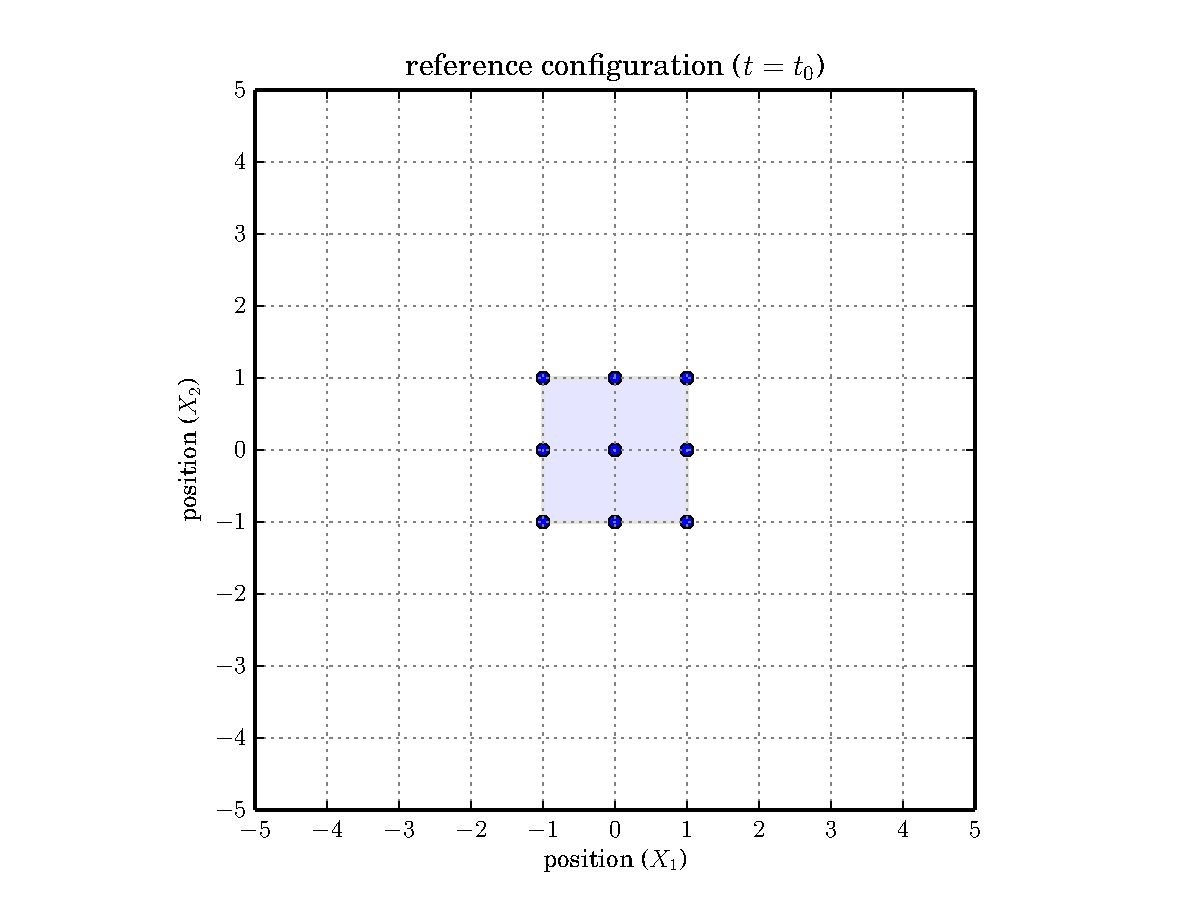
\includegraphics[width=\textwidth]{fig/configuration_reference.pdf}
  \end{center}
  \label{fig:configuration_reference}
\end{figure}

The most elementary displacement is homogeneous, when 
$\tMbold = \vid$ 
and
$\vb = \vzero$, then $\vu = \vzero$.
In this case $\vvarphi = \vX$ and the motion is trivial (and
uninteresting).  Nonetheless, this is a simple first case to consider.

\subsection{Offset}
\label{section:offset}
Next, consider $\vb \neq \vzero$, while
retaining $\tMbold = \vid$.   For the concrete example 
in Fig.~(\ref{fig:configuration_current}), let 
$\vb = \langle b_1, b_2 \rangle\transpose = 
\langle 3, 2 \rangle\transpose$.
In this case, we see the placement $\vvarphi$ moves right and up
on the page, relative to the reference configuration $\vX$, by 
an amount of 3 and 2, respectively.
\begin{figure}[htb]
  \caption{Current configuration shown in red, with reference 
  configuration shown in blue and retained for context.}
  \begin{center}
    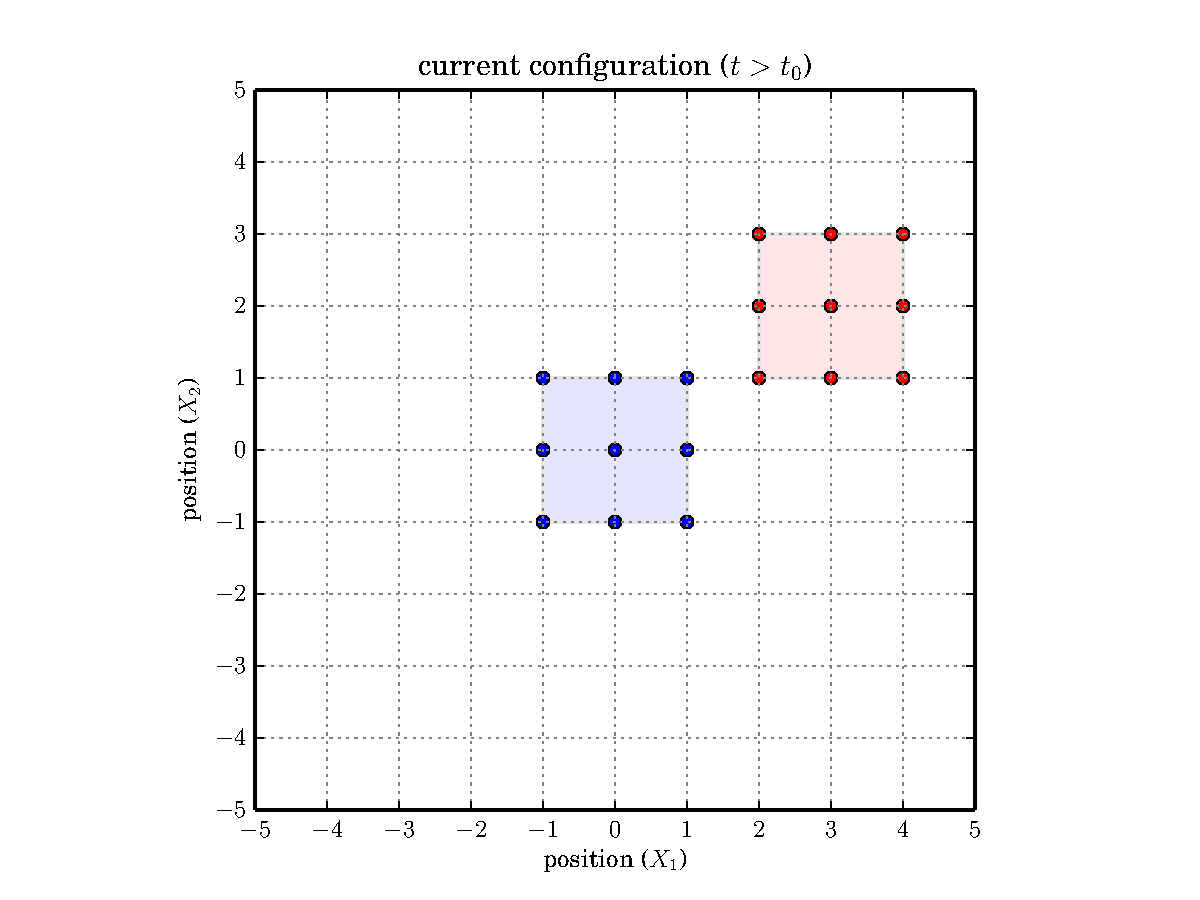
\includegraphics[width=\textwidth]{fig/configuration_current.pdf}
  \end{center}
  \label{fig:configuration_current}
\end{figure}


\clearpage
\subsection{Stretch}
Consider now $\tMbold = \lambda \vid$ and $\vb = \vzero$.  
This describes {\bf volumetric} response, also known 
as a {\bf dilitational} response.  The parameter $\lambda \in \real$
causes the current configuration to change volume as
\begin{itemize}
 \item $\lambda > 0$ expansion,
 \item $\lambda = 0$ identity,
 \item $\lambda < 0$ contraction.
\end{itemize}
Notice that $\lambda$ describes the ``slope'' of the mapping from
reference to current configurations.  In the case that $\lambda \rightarrow
+\infty$, the volume grows infinite.  In the case that $\lambda \rightarrow
-\infty$, the volume grows to zero.
For concreteness, consider $\lambda = 2$.  The volumetric expansion
is shown in Fig.~\ref{fig:configuration_volumetric}.

\begin{figure}[htb]
  \caption{Current configuration shown in red, with reference 
  configuration shown in blue and retained for context.}
  \begin{center}
    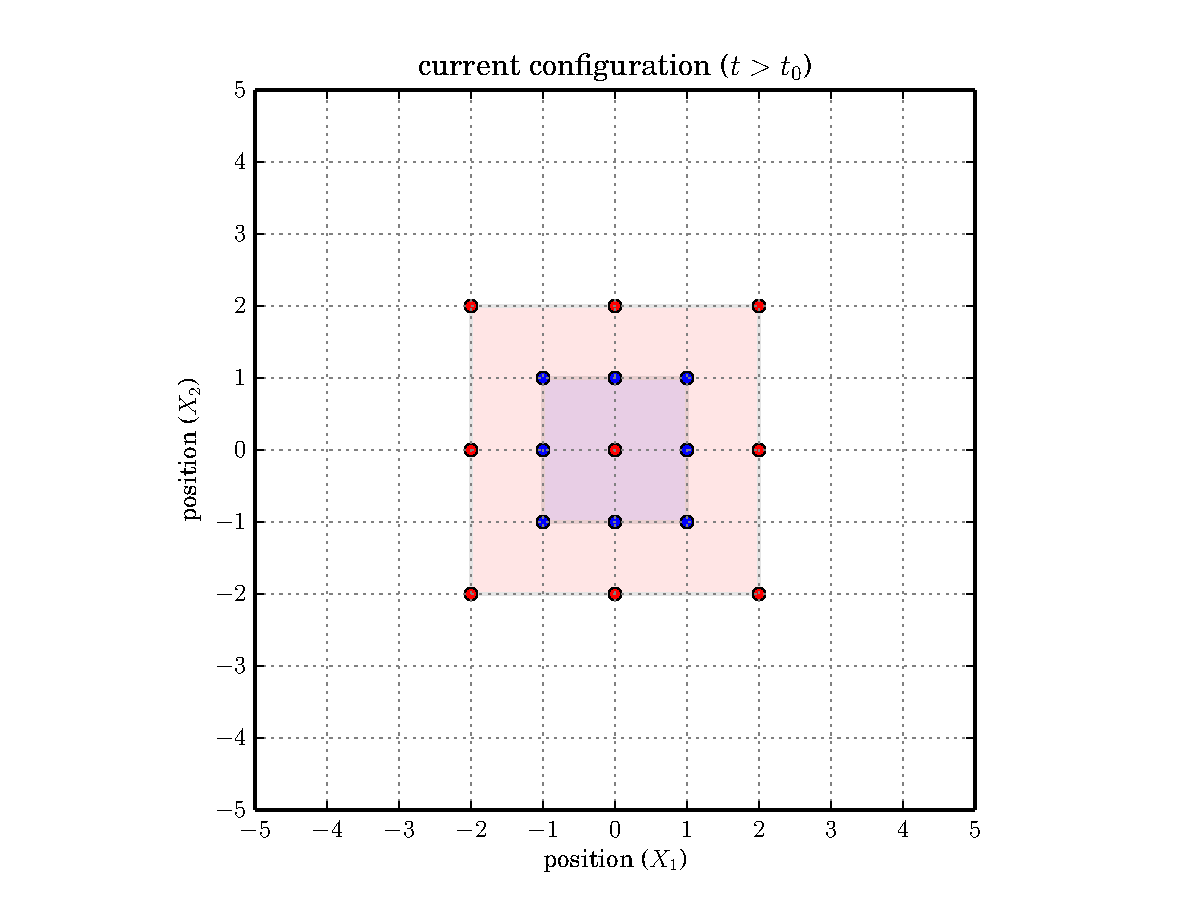
\includegraphics[width=\textwidth]{fig/configuration_volumetric.pdf}
  \end{center}
  \label{fig:configuration_volumetric}
\end{figure}

The area in the reference configuration was $2 \times 2 = 4$, 
whereas the area in the current configuration was $4 \times 4 = 16$.   


Next consider a slightly different form of $\tMbold$, such that
\be
 \tMbold 
 = 
 \left[
 \begin{tabular}{cc}
  $\lambda_1$ & 0 \\
  0 & $\lambda_2$
 \end{tabular}
 \right].
\ee
We keep the offset as $\vb = \vzero$.

For concreteness, consider $\lambda_1 = 2$
and $\lambda_2 = \half$.   The combined expansion and compression
is shown in Fig.~\ref{fig:configuration_stretch}.

\begin{figure}[htb]
  \caption{Current configuration shown in red, with reference 
  configuration shown in blue and retained for context.}
  \begin{center}
    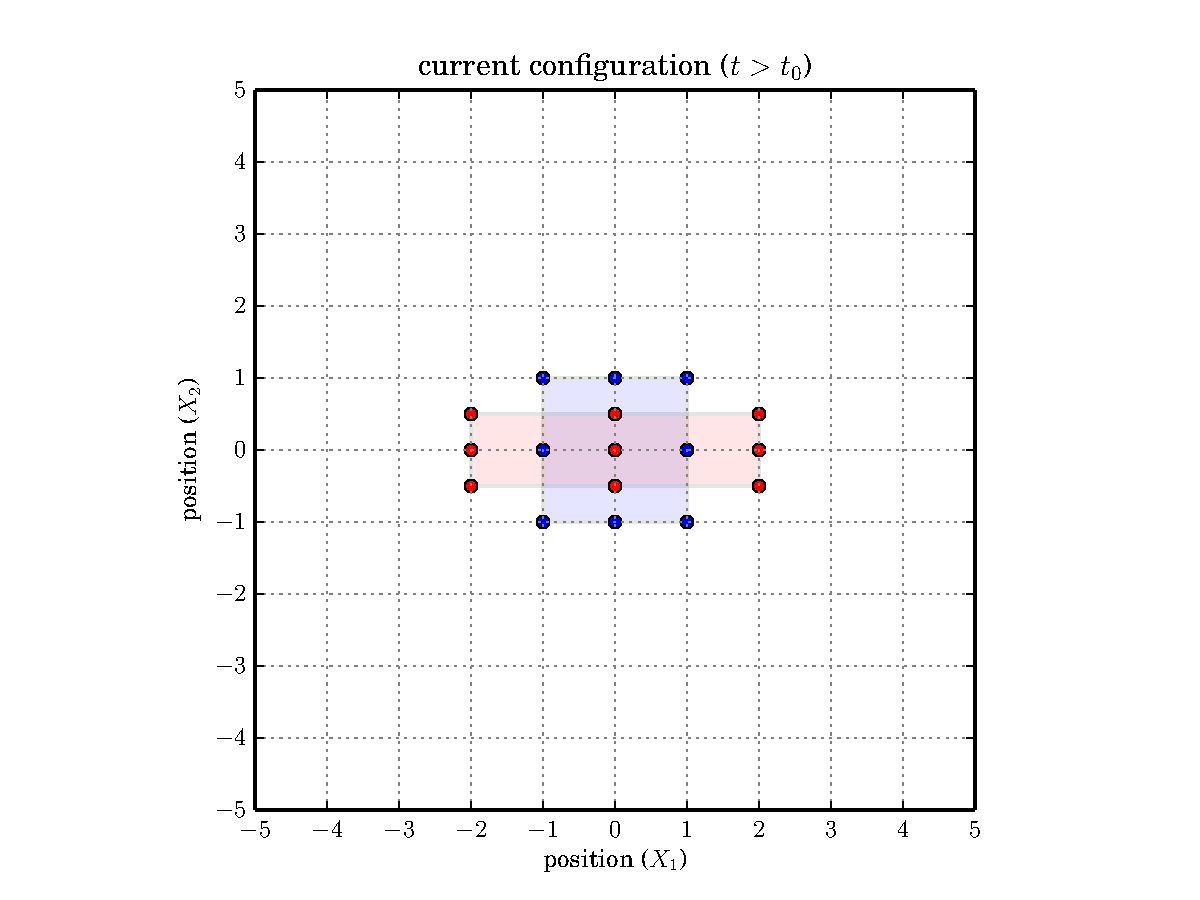
\includegraphics[width=\textwidth]{fig/configuration_stretch.pdf}
  \end{center}
  \label{fig:configuration_stretch}
\end{figure}

The area in the reference configuration was $2 \times 2 = 4$, 
whereas the area in the current configuration was $4 \times 1 = 4$.   
Out of coincidence, we have chosen stretches along the 
two axes such that the area does not change although the dimensions
and thus shape have changed.  This is an example of an 
{\bf isochoric} motion.  The roots {\em iso- (equal)} and {\em choro- (space)} 
describe a process from initial state $0$ to final state $1$
where the volume remains constant.  

Now, the motion as we have described it, doesn't yet show the {\em path}
taken between the reference and current configuration.  To 
get that detail, we would need to introduce the time parameter $t$, 
which we have suppressed for now.  
However, if we were to say the time interval is simply two points 
$t_0$ and $t_1$, we can create (the rather course) path between these
two states $0$ and $1$, and connect with the isochoric process
$PV$ diagram in thermodynamics, shown in Fig.~\ref{fig:PV_isochoric}.

\begin{figure}[htb]
  \caption{Isochoric process from initial state (reference configuration) $0$ to
  final state (current configuration) $1$.}
  \begin{center}
    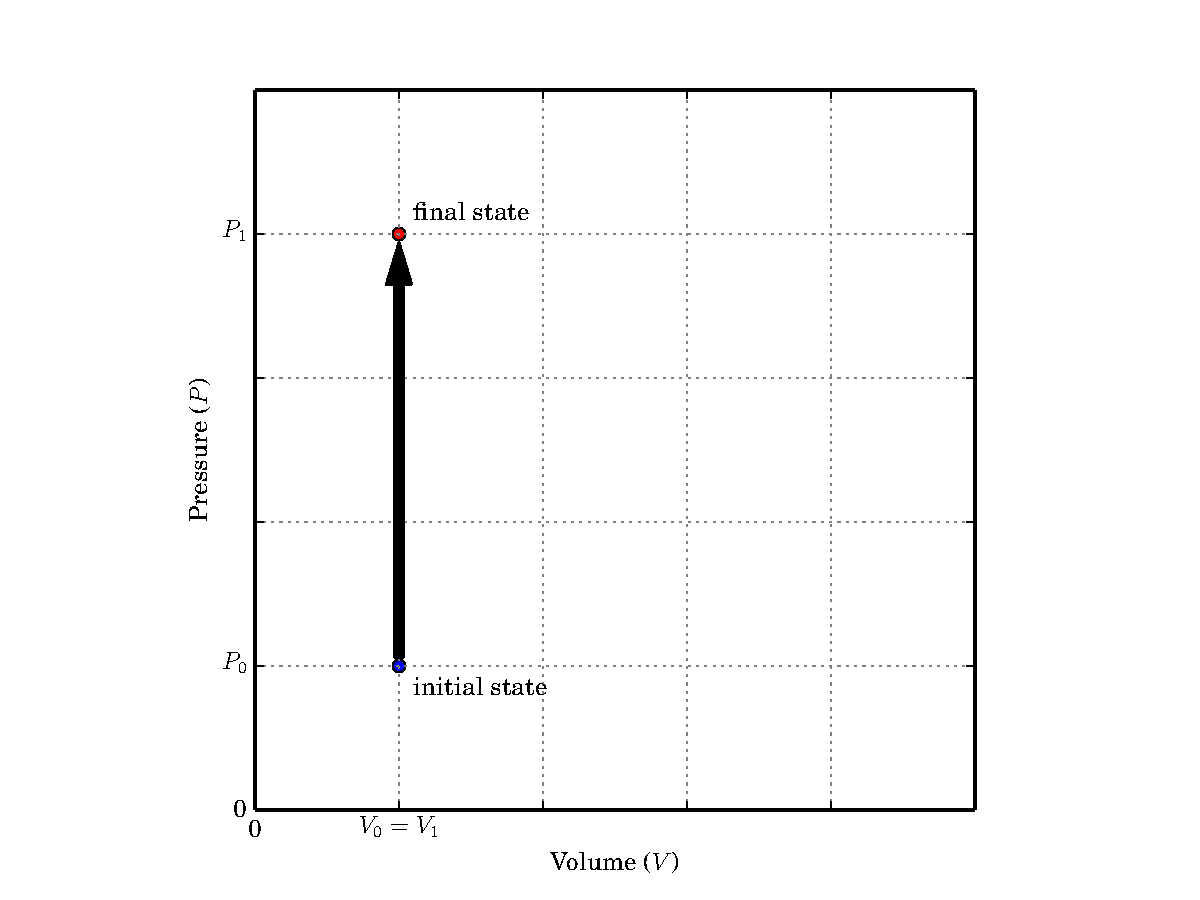
\includegraphics[width=\textwidth]{fig/PV_isochoric.pdf}
  \end{center}
  \label{fig:PV_isochoric}
\end{figure}

We have yet to introduce and define pressure $P$, so this 
connection may be tenuous at the moment.  Nonetheless, we
introduce this connection now to motivate the single idea that
isochoric motions will play an important role in our later work.

\subsection{Rotation}

\section{Deformation Gradient}
To each configuration, we define a deformation gradient 
$\tFbold: \cB \times \interval \mapsto \Mthreeplus$ 
such that
\begin{equation}
\tFbold 
\defe 
\Grad \vvarphi
\;\; \Longleftrightarrow \;\;
\tF_{iJ} 
\defe 
\frac{\partial \varphi_i}{\partial X_J}.
\label{eq:deformation_gradient}
\end{equation}
Remarks:
\begin{itemize}
\item Lower case indices represent components of tensors in the
current configuration whereas upper case indices represent
components of tensors in the reference configuration.  Real, 
square matrices of dimension three and positive determinants
are denoted $\Mthreeplus$.  
\item We define gradients taken in the reference configuration 
as $\Grad(\cdot) = \partial (\cdot) / \partial X_J$ 
to distinguish from gradients taken in the current
configuration, denoted simply as $\grad(\cdot) = 
\partial (\cdot) / \partial x_j$.
\item All configurations must be admissible in the sense that the Jacobian
of the deformation $J$ much be positive
\begin{equation}
 J \defe \det \tFbold > 0.
\end{equation}
This requirement keeps the deformations from mapping the body to
a single, infinitesimally small point ($J=0$) or turning the
body inside-out ($J<0$).  
\end{itemize}

From the displacement field in 
(\ref{eq:displacement}), we see that 
the relationship between the displacement gradient and the 
deformation gradient is given by
\be
\Grad \vu = \Grad \vvarphi - \vid = \tFbold - \vid.
\ee

\section{Strain}
\subsection{Right Cauchy-Green}
A standard strain measure is the right Cauchy-Green
strain tensor
\begin{equation}
 \tCbold 
 \defe 
 \tFbold\transpose \tFbold
 \;\; \Longleftrightarrow \;\;
 \tC_{IJ} 
 \defe 
 \tF_{Ii} \; \tF_{iJ}. 
\end{equation}
The right Cauchy-Green strain tensor $\tCbold$ gets its name from the 
fact that the deformation gradient $\tFbold$ sits to the right.  
Note that this strain tensor is defined in the reference configuration.
The right Cauchy-Green strain tensor can be written
explicitly as reference gradients of the motion 
$\vvarphi$ or displacement $\vu$:
\begin{align}
\tCbold &\overset{(\ref{eq:deformation_gradient})}{=} 
(\Grad \vvarphi)\transpose \Grad \vvarphi \nonumber \\
    &= (\Grad \vu + \vid)\transpose (\Grad \vu + \vid) \nonumber \\
    &= (\Grad \vu)\transpose\Grad \vu + \Grad \vu + (\Grad \vu)\transpose 
    + \vid
    \label{eq:C_in_terms_of_u}
\end{align}

\subsection{Left Cauchy-Green}
In contrast, a left Cauchy-Green
strain tensor $\tbbold$ can be defined with the 
deformation gradient $\tFbold$
sitting on the left.
\be
 \tbbold \defe \tFbold \tFbold\transpose
 \;\; \Longleftrightarrow \;\;
 \tb_{ij} \defe \tF_{iJ} \; \tF_{Jj}.
 \label{eq:left_cauchy_green}
\ee
Note that this strain measure is defined in the current 
configuration.

\subsection{Lagrangian (Green) Strain Tensor}
The Lagrangian (Green) strain tensor,
\begin{equation}
 \tEbold 
 \defe
 \half (\tCbold - \vid)
 \;\; \Longleftrightarrow \;\;
 \tE_{IJ} 
 \defe 
 \half(\tC_{IJ} - \delta_{IJ}),
\end{equation}
is closely related to the right Cauchy-Green strain tensor
and is often used in defining constitutive
law relationships because the measure, when linearized
about the reference configuration, coincides with the
small strain tensor of linear deformation elasticity, 
denoted~$\ve{\epsilon}$ and defined in (to come).
This relationship can be seen as follows:
\begin{align}
 2 \tEbold 
     &\overset{(\ref{eq:C_in_terms_of_u})}{=} 
     (\Grad \vu)\transpose \Grad \vu + 
     \Grad \vu + (\Grad \vu)\transpose + \vid - \vid,
     \label{eq:E_expanded} \\
 %\ve{\epsilon}  
 2 \tEbold_{\tiny \mbox{LIN}}
     %&\overset{\tiny \mbox{LIN}}{=} 
     &= 
     \Grad \vu + (\Grad \vu)\transpose,
     \label{eq:small_strain}
\end{align}
where the higher-order (first) term in (\ref{eq:E_expanded}) is set
to zero to achieve (\ref{eq:small_strain}).

\subsection{Eulerian (Almansi) Strain Tensor}
The Eulerian (Almansi) strain tensor,
\be
 \tebold 
 \defe 
 \half (\vid - \tbbold^{-1} )
 \;\; \Longleftrightarrow \;\;
 \te_{ij} 
 \defe 
 \half \left(\delta_{ij} - (\tb_{ij})^{-1}\right),
\ee
can likewise be used to approximate the small strain tensor
$\ve{\epsilon}$ by combining (\ref{eq:left_cauchy_green}) and
(\ref{eq:deformation_gradient}) as follows:
\begin{align}
 2 \tebold &=
     \vid - \left[ \Grad \vvarphi 
     (\Grad \vvarphi)\transpose \right]^{-1} \nonumber \\
     &= 
     \delta_{ij} 
       - \left[ \frac{\partial \varphi_i}{\partial X_J}
                \frac{\partial \varphi_j}{\partial X_J}
         \right]^{-1} % \nonumber \\
     =
      \delta_{ij} 
       - \left[ \frac{\partial X_J}{\partial \varphi_i}
                \frac{\partial X_J}{\partial \varphi_j}
         \right] 
	    \nonumber \\ 
     &\overset{(\ref{eq:displacement})}{=}
      \vid 
       - \left[
                (\vid - \grad \vu) (\vid - \grad \vu)\transpose
         \right]
	   \nonumber \\ 
     &=
     \grad \vu + \grad \vu\transpose - 
     \grad \vu \grad \vu\transpose 
     \label{eq:b_expanded} \\
 %\ve{\epsilon}  
 2 \tebold_{\tiny \mbox{LIN}} 
     %&\overset{\tiny \mbox{LIN}}{=} 
     &=
     \grad \vu + (\grad \vu)\transpose,
     \label{eq:small_strain_two}
\end{align}
where higher-order (quadratic) term in (\ref{eq:b_expanded}) is set
to zero to achieve (\ref{eq:small_strain_two}).

\subsection{When Strains are Small}

\subsection{Seth-Hill Strain Tensor Family}
Seth and Hill showed that the 
Lagrangian (Green) and Eulerian (Almansi)
strain tensors are special cases of the so-called
Seth-Hill family of strain measures, defined as
\be
 \tEbold_{(m)} \defe \frac{1}{2 m}
 \left(\tUbold^{2 m} - \vid \right)
 = 
 \frac{1}{2 m} 
 \left(\tCbold^m - \vid \right).
\ee
Then
\begin{align}
 \tEbold_{(1)} = 
 \half \left(\tUbold^{2} - \vid \right) = 
 \half \left(\tCbold - \vid \right) 
 & \hspace{1cm} \mbox{{\bf Lagrangian (Green)}}, \\
 \tEbold_{(1/2)} = 
 \left(\tUbold - \vid \right)  = 
 \left(\sqrt{\tCbold} - \vid \right) 
 & \hspace{1cm} \mbox{{\bf Biot}}, \\
\tEbold_{(0)} = 
 \ln\tUbold   = 
 \half \ln\tCbold
 & \hspace{1cm} \mbox{{\bf Logarithmic, Natural, True, Hencky}}, \\
\tEbold_{(-1)} = \half 
 \left(\vid - \tUbold^{(-2)} \right) 
 & \hspace{1cm} \mbox{{\bf Eulerian (Almansi)}}.
\end{align}


\subsubsection{The Linearized Lagrangian (Green) Strain Tensor 
Creates Nonzero Strains under Rigid Body Rotations}

Because it takes on nonzero values under finite rotation,
the linearized strain tensor 
should not be used for geometrically nonlinear analysis.
These nonzero values are completely artificial and strictly
an artifact of using a linear strain definition with
geometrically nonlinear motions.   This result is shown as follows:

Let $\tRbold = \tRbold(t)$ be a two-dimensional, 
rigid body rotation parameterized by time $t$
and scaled by constant $\omega = 2 \pi$~radians per second.  
Then, the motion $\vvarphi$ of a body can be written as
\be
 \vvarphi(\vX, t) = \tRbold(t) \vX 
 \;\; \Longleftrightarrow \;\;
 \left\{
 \begin{tabular}{c}
 $x_1$ \\
 $x_2$
 \end{tabular}
 \right\}
 = 
 \left[
 \begin{tabular}{rr}
 $\cos \omega t$ & $\sin \omega t$ \\
 $-\sin \omega t$ & $\cos \omega t$ 
 \end{tabular}
 \right]
 \left\{
 \begin{tabular}{c}
 $X_1$ \\
 $X_2$
 \end{tabular}
 \right\}.
\ee
Then the deformation gradient $\tFbold = \tFbold(t)$ is a function of time
alone,
\be
 \tFbold(t)
 \;\; \Longleftrightarrow \;\;
 \tF_{iJ} 
 = 
 \left[
 \begin{tabular}{rr}
 $\tF_{11}$ & $\tF_{12}$ \\
 $\tF_{21}$ & $\tF_{22}$ 
 \end{tabular}
 \right]
 =
 \left[
 \begin{tabular}{rr}
 $\cos \omega t$ & $\sin \omega t$ \\
 $-\sin \omega t$ & $\cos \omega t$ 
 \end{tabular}
 \right].
\ee
The linearized strain tensor is found to be 
\begin{align}
 2 \tEbold_{\tiny \mbox{LIN}}
 &= \Grad \vu + (\Grad \vu)\transpose, \\
 &= \tFbold - \vid + 
     \left(\tFbold - \vid \right)^T, \\
 &= \tF_{iJ} - \delta_{iJ} + \tF_{Ji} - \delta_{Ji}, \\ 
 &= 
 \left[
 \begin{tabular}{rr}
 $\cos \omega t$ & $\sin \omega t$ \\
 $-\sin \omega t$ & $\cos \omega t$ 
 \end{tabular}
 \right]
 +   
 \left[
 \begin{tabular}{rr}
 $\cos \omega t$ & $-\sin \omega t$ \\
 $\sin \omega t$ & $\cos \omega t$ 
 \end{tabular}
 \right]
 -   
 \left[
 \begin{tabular}{rr}
 $2$ & $0$ \\
 $0$ & $2$ 
 \end{tabular}
 \right], \\
 &=
 2 \left( \cos \omega t - 1 \right) \vid.
\end{align}
Now, for small angles, $\omega t \approx 0$, which is
for small deviations $x_1 \approx X_1$, $x_2 \approx X_2$, then
$\tEbold_{\tiny \mbox{LIN}} = \ve{0}$ for rigid body rotations.
However, for arbitrary finite angles, $\omega t \neq 0$,
and the linearized strain tensor
$\tEbold_{\tiny \mbox{LIN}}$ reports nonzero strain for rigid
body rotations, which is nonsensical.

A correct strain tensor will report zero strain for rigid body
rotations.  One such strain tensor is the fully nonlinear Lagrangian
(Green) strain tensor.  This result is shown as follows:
\begin{align}
 2 \tEbold &= \tFbold\transpose\tFbold - \vid \\
 &= 
 \left[
 \begin{tabular}{rr}
 $\cos \omega t$ & $-\sin \omega t$ \\
 $\sin \omega t$ & $\cos \omega t$ 
 \end{tabular}
 \right]
 \left[
 \begin{tabular}{rr}
 $\cos \omega t$ & $\sin \omega t$ \\
 $-\sin \omega t$ & $\cos \omega t$ 
 \end{tabular}
 \right]
 -   
 \left[
 \begin{tabular}{rr}
 $1$ & $0$ \\
 $0$ & $1$ 
 \end{tabular}
 \right] = \ve{0}. 
\end{align}

\section{Stress}

\section{Hyperelasticity}



%  
\chapter{Balance Laws}

%\newcommand{\phibar}{\bar{\phi}}
%\newcommand{\phistar}{\overset{*}{\phi}}
\newcommand{\phistar}{\phi^*}
\newcommand{\phihat}{\hat{\phi}}

In this section, we posit the {\bf Master Balance Law} 
in general form.  Also called ``conservation of anything,'' this
description assumes an arbitrary control volume $V \in \realthree$
with boundary $\partial V$.  What follows is the so-called 
Eulerian formulation, illustrated in Fig.~\ref{fig:mass_balance}, 
which assumes the control volume, 
while arbitrary in its placement in space, is {\bf fixed} 
in space.\footnote{The connection to the Lagrangian formulation, 
in which the control is not fixed in space, but instead, 
moves through space as the body to which it
is attached moves through space, is examined in the sequel.} 
\begin{figure}[htb]
  \begin{center}
    %\begin{overpic}[width=0.85\textwidth, grid, tics=10]{fig/mass_balance}
    \begin{overpic}[width=0.85\textwidth,natwidth=566,natheight=283]{fig/mass_balance.pdf}
      \put(22, 36){flux in}
      \put(85, 26){flux out}
      \put(44,  2){$V$}
      \put(54.5, 47){$\vnhat$ on $\partial V$}
      %\put(50.5,  24){$g$}
      \put(49.5,  23.8){$\phi^*$}
      %
    \end{overpic}
  \end{center}
  \caption{Concept of a fixed control volume of the Eulerian formulation.}
  \label{fig:mass_balance} 
\end{figure}

Now, let 
\begin{itemize}
\item $\phi(\vx, t)$ be the description of some physical quantity 
per unit volume, which can in general be a scalar, vector, or tensor quantity, 

\item $\phistar(\vx, t)$ be the generation (depletion) {\em rate} of the 
physical quantity per unit volume, 

\item $\phihat(\vx, t)$ be the physical quantity per unit volume 
that flows across the boundary with rate (velocity) $\vv(\vx, t)$, and 

\item $\partial V$ be the boundary of the control volume, 
with outward pointing surface normal unit vector $\vnhat(\vx, t)$.  
\end{itemize} 
The time rate of change of the quantity $\phi(\vx,t)$ within the 
differential control volume $dV$ is then equal to 
\begin{itemize}
\item {\bf generation}---the rate at which the quantity is generated (or depleted) 
within the control volume by the point source (point sink), plus
\item {\bf flux}---the rate at which the quantity is either carried into (or out of) 
the volume across the volume's differential surface area $dA$.
\end{itemize}
These words, stated mathematically, are
\be
 \underset{\mbox{\footnotesize rate}}{\underbrace{\frac{d}{dt} 
 \int_{V} \phi(\vx,t) \; dV}}
  \;\; = \;\;  
   \underset{\mbox{\footnotesize source}}{\underbrace{\int_{V} 
   \phistar(\vx,t) \; dV}}
   \;\; - \;\;
   \underset{\mbox{\footnotesize flux}}{\underbrace{\int_{\partial V} 
   %\left(
   \phihat(\vx,t) \; \vv(\vx,t) 
   %\right) 
   \cdot \vnhat \; dA}}
   ,
\ee
which is the general form of the 
{\bf Master Balance Law}.  We adopt the following sign convention 
to impart consistency:
\begin{itemize}
\item For positive time rate of change of the quantity $\phi(\vx,t)$, 
the generation $\phistar(\vx,t)$ is trivially positive.  
For quantity $\phihat(\vx,t)$ carried
{\em into} the control volume, the inner product of $\vv$ with $\vnhat$ is
negative, thus a negative outside of the flux integral is used.  
\item Likewise, for a negative time rate of change of 
quantity $\phi(\vx,t)$, 
the generation $\phistar(\vx,t)$ is negative.  
And, for the quantity $\phihat(\vx,t)$ 
carried {\em out of} the control volume, the inner product of $\vv$ with
$\vnhat$ is positive, thus the negative outside of the flux integral 
provides sign consistency.  
\end{itemize}

\section{Balance Law Metaphor}
Here we present the Master Balance Law by way of metaphor.  
Let the volume $V$ be the geographic region of Oregon, 
with boundary $\partial V$ that touches the state borders of
Washington, Idaho, Nevada, and California 
in the United States.\footnote{In this oversimplified
metaphor, we assume flux does not occur via the western seaboard nor via the air.} 
Let $\phi$ be the number of people living in the state of Oregon.
The change in population $\Delta \phi$ over some time interval $\Delta t$ 
is equal to the 
net generation rate $\phistar$ (number of births less the number of deaths
in the time interval), plus the net population flux rate $\phihat \vv$
(the number of people moving to Oregon less
the number of people moving from Oregon within the time interval).

\section{Conservation of Mass}
Let us now apply the Master Balance Law to the physical 
quantity of mass, and develop a relationship for 
{\bf conservation of mass},
a concept where mass is neither created nor destroyed.  
The physical quantity of mass per unit volume is 
density $\rho(\vx,t)$.  Thus, we substitute $\rho(\vx,t)$ 
for $\phi(\vx,t)$ in the foregoing Master Balance Law.

\be
\begin{tabular}{cl|l}
 &
 {\bf Assumption}
 &
 {\bf Expression} \\ \hline \hline
 (1) 
 &
 No mass generation or depletion. 
 &
 $\rho^*(\vx,t) = 0$
 \\ \hline
 (2)
 &
 Mass can flow in and out of the boundaries.
 &
 $\rho(\vx, t) \vv(\vx, t) \cdot \hat{\vn}(\vx, t) \neq 0$
\end{tabular}
\ee

\begin{Hresult}
Conservation of mass in the current configuration is stated as 
\be
   \frac{\partial \rho(\vx,t)}{\partial t} + \grad \cdot 
   %\left[ \; \rho(\vx,t) \;  \vv(\vx,t) \; \right] 
   \left( \; \rho(\vx,t) \;  \vv(\vx,t) \; \right)
 = 
 0
 \;\; \Longleftrightarrow \;\; \rho_{,t} + (\rho \; v_{i})_{,i} = 0.
 \label{eq:mass_conservation}
\ee
\end{Hresult}

\begin{Hproof}
For mass to be conserved, 
mass within a control volume is neither created nor destroyed, thus the source
term is identically zero.  Thus, increases (decreases) in the mass rate 
term are produced only by flux of mass in through (out from) the boundary. 
The idea, stated mathematically, is
\be
 \underset{\mbox{\footnotesize rate}}{\underbrace{\frac{d}{dt} 
 \int_{V} \rho(\vx,t) \; dV}}
  \;\; = \;\;  
   \underset{\mbox{\footnotesize source = 0}}{\underbrace{\int_{V} 
   \rho^*(\vx,t) \; dV}}
   \;\; - \;\;
   \underset{\mbox{\footnotesize flux}}{\underbrace{\int_{\partial V} 
   %\left[\; \rho(\vx,t) \; \vv(\vx,t) \; \right] \cdot \vnhat(\vx,t) \; dA}}
   \rho(\vx,t) \; \vv(\vx,t) \cdot \vnhat(\vx,t) \; dA}}
   .
\ee
The Divergence Theorem is used to write the flux term surface integral 
as a volume integral, thus
\be
 \underset{\mbox{\footnotesize rate}}{\underbrace{\frac{d}{dt} 
 \int_{V} \rho(\vx,t) \; dV}}
  \;\; = \;\;  
   0
   \;\; - \;\;
   \underset{\mbox{\footnotesize flux}}{\underbrace{\int_{V} 
   %\grad \cdot \left[\;\rho(\vx,t) \; \vv(\vx,t) \; \right] \; dV}}
   \grad \cdot \left(\;\rho(\vx,t) \; \vv(\vx,t) \; \right) \; dV}}
   .
\ee
Because $V$ is fixed in an inertial frame, the foregoing equation can be 
rewritten with the rate time derivative inside the integral, thus
\be
 \int_{V} \left(
   \frac{\partial \rho(\vx,t)}{\partial t} + \grad \cdot 
   %\left[ \; \rho(\vx,t) \;  \vv(\vx,t) \; \right] \; \right) \; dV 
   \left( \; \rho(\vx,t) \;  \vv(\vx,t) \; \right) \; \right) \; dV 
 = 
 0
 .
\ee
Finally, arbitrariness of $B_t$ 
requires that the integrand is identically zero, thus
\be
   \frac{\partial \rho(\vx,t)}{\partial t} + \grad \cdot 
   %\left[ \; \rho(\vx,t) \;  \vv(\vx,t) \; \right] 
   \left( \; \rho(\vx,t) \;  \vv(\vx,t) \; \right)
 = 
 0
 \;\; \Longleftrightarrow \;\; \rho_{,t} + (\rho \; v_{i})_{,i} = 0,
 \label{eq:mass_conservation_two}
\ee
which is the result.
\end{Hproof}


\begin{Hremark}
Conservation of mass is also called the {\bf continuity equation}.  
Some texts will recast the continuity equation by defining a 
{\bf material derivative} of density as follows:  Since
$\rho = \rho(\vx, t)$, then 
\be
 \dot \rho = \frac{\partial \rho}{\partial \vx} \frac{\partial \vx}{\partial t} 
 + \frac{\partial \rho}{\partial t} \defe \frac{D \rho}{Dt}.
\ee
With arguments $(\vx, t)$ suppressed for brevity, (\ref{eq:mass_conservation}) 
can be expanded to give 
\be
  \frac{\partial \rho}{\partial t} + 
  \grad \rho \cdot \vv + \rho \; \grad \cdot \vv = 
  \underset{\defe \; \dot\rho}{\underbrace{
  \frac{\partial \rho}{\partial t} + 
  \frac{\partial \rho}{\partial \vx} \frac{\partial \vx}{\partial t}}} +
  \rho \grad \cdot \vv = 0,
\ee
or simply
\be
\dot \rho + \rho \grad \cdot \vv = 0.
\ee
\end{Hremark}


\section{Conservation of Linear Momentum}

\section{Conservation of Angular Momentum}

\be
\begin{tabular}{cl|l}
 &
 {\bf Assumption}
 &
 {\bf Expression} \\ \hline \hline
 (1) 
 &
 Point torques are zero. 
 &
 $\vx \times \vfext = \vzero$
 \\ 
\end{tabular}
\ee
\begin{Hresult}
The Cauchy stress tensor $\vsigma(\vx, t)$ is symmetric, thus
 $\vsigma = \vsigma\transpose$.
\end{Hresult}

\section{Conservation of Energy}
\be
\begin{tabular}{cl|l}
 &
 {\bf Assumption}
 &
 {\bf Expression} \\ \hline \hline
 (1) 
 &
 Energy is neither created nor destroyed.
 &
  
 \\ 
\end{tabular}
\ee

 
%  \chapter{Plasticity}

We first focus on plasticity in one dimension, 
as opposed to fully three-dimensional plasticity, 
to emphasize concepts while being
as mathematically simple as possible.  
After the concepts are clear, the extension of the mathematics from
one- to three-dimensions can be made naturally.  

\section{Perfect Plasticity}
The extension of elasticity to plasticity is made by way of 
{\em perfect} plasticity.
Conceptually, perfect plasticity in the constitutive stress-strain 
relationship is obtained by ``capping'' the
elastic response function at some yield stress 
(to be defined later as $\sigma_y$).  Beyond the yield stress, the 
stress response function is perfectly horizontal.  
Increases in strain produce no increase in stress
beyond the yield stress.  


\subsection{Deformation Measures}
Let the body $\Omega$ have strain measure 
$\hstrain : \Omega \rightarrow \real$ 
in one dimension be defined as a ratio of change in length, that is 
the difference between the new (deformed, current configuration) 
length $\ell$ of body $\Omega$ and the original (undeformed, reference 
configuration) length $L$, divided by the original length, 
\be
 \hstrain \defe \frac{\ell - L}{L}.
 \ee
 The total strain $\hstrain$ in the body be defined as an 
 additive decomposition of elastic strain $\hstraine$ and 
plastic strain $\hstrainp$, 
\be
 \label{eq:smallStrainAddition}
 \hstrain \defe \hstraine + \hstrainp.
\ee


\subsection{Constitutive Law}
Then, the traditional stress-strain relationship, $\sigma = E \hstraine$, 
can be rewritten as
\be
 \label{eq:stressStrain}
 \sigma = E \left( \hstrain - \hstrainp \right).
\ee
A change in the configuration of the plastic element 
(see  Fig.~\ref{fig:plastic_slider})
can only occur if the notion of {\bf slip rate} is
allowed.

%\begin{figure}[htb]
% \psfrag{a}{$\sigma$}
% \psfrag{b}{$\sigma_y$}
% %\fbox{\begin{minipage}{0.95\columnwidth}\centering
% \begin{center}
% \includegraphics[width=2.8in]{fig/plasticityFrictionElement.eps}
% \end{center}
% \caption{Phenomenological model of a friction element.  A unit cross-sectional
% area is assumed.  Motion in the friction 
% element occurs only if the friction force, $\sigma_y$, 
% is exceeded.  The motion, in rate form, is
% referred to as the slip rate. Note that we employ a slight abuse of 
% notation by using $\sigma$ to describe a force $F$, since the cross-sectional area $A$ is
% unity, $F = \sigma A \implies \sigma \cdot 1 = \sigma$.}
% \label{fig:plasticFrictionElement_old} % label must come after caption 
% %\end{minipage}
% %} % \fbox
%\end{figure}


\begin{figure}[htb]
  \begin{center}
  %\begin{overpic}[width=0.5\textwidth, grid, tics=10]{fig/plastic_slider}
  %\begin{overpic}[width=0.5\textwidth,natwidth=144,natheight=51]{fig/plastic_slider.pdf}
  \begin{overpic}[width=0.5\textwidth]{fig/plastic_slider.pdf}
    \put( 4, 13){$\sigma$}
    \put(95, 13){$\sigma$}
    \put(47, 23){$\sigma_y$}
  \end{overpic}
  \end{center}
 \caption{Phenomenological model of a friction element.  A unit cross-sectional
 area is assumed.  Motion in the friction 
 element occurs only if the friction force, $\sigma_y$, 
 is exceeded.  The motion, in rate form, is
 referred to as the slip rate. Note that we employ a slight abuse of 
 notation by using $\sigma$ to describe a force $F$, since the 
 cross-sectional area $A$ is
 unity, $F = \sigma A \implies \sigma \cdot 1 = \sigma$.}
 \label{fig:plastic_slider} % label must come after caption 
\end{figure}

%\begin{figure}[htb]
%\begin{center}
%  \psfragfig[width=6cm]{fig/plasticityFrictionElement}{% the .eps file
%    \psfrag{a}{$\sigma$}
%    \psfrag{b}{$\sigma_y$}
%  } % psfragfig
%\end{center}
% \caption{Phenomenological model of a friction element.  A unit cross-sectional
% area is assumed.  Motion in the friction 
% element occurs only if the friction force, $\sigma_y$, 
% is exceeded.  The motion, in rate form, is
% referred to as the slip rate. Note that we employ a slight abuse of 
% notation by using $\sigma$ to describe a force $F$, since the cross-sectional area $A$ is
% unity, $F = \sigma A \implies \sigma \cdot 1 = \sigma$.}
% \label{fig:plasticFrictionElement} % label must come after caption 
%\end{figure}
%


That is, {\em assume} that $\hstrainp(t)$ is a 
function of time on interval $[0, T] \subset \real$.  
Then from~(\ref{eq:smallStrainAddition}) and~(\ref{eq:stressStrain}), 
time evolution expressions $\hstrain(t)$ and $\sigma(t)$ exist, respectively.  
Finally, the presence of evolution equations allows the constitutive law 
in~(\ref{eq:stressStrain}) to be
written as
\be
 \sigmadot = E \left( \hstraindot - \hstrainpdot \right).
 \label{eq:stressStrainRate}
\ee
This form of the constitutive equation will 
become useful for quantifying plastic 
flow, as seen below in~(\ref{eq:PhiChainRule}).

%\begin{figure}[htb]

%%\begin{figure*}[h!]
% \psfrag{a}{(b) slip rate $\gammadot \geq 0$}
% \psfrag{b}{(a) yield function $\Phi(\sigma) \leq 0$}
% \psfrag{c}{(c) consistency}
% \psfrag{g}{$\gammadot$}  
% \psfrag{p}{$\Phi$} 
% %\fbox{\begin{minipage}{0.98\textwidth}\centering
% \begin{center}
% \includegraphics[width=5.5in]{fig/plasticunion.eps}
% \end{center}
% \caption{Unilateral conditions (a) $\Phi(\sigma) \leq 0$ and 
% (b) slip rate $\gammadot \geq 0$.  
%  The complementarity condition, $\gammadot \; \Phi(\sigma) = 0$, 
%  is shown in~(c).}
% \label{fig:plasticunion} % label must come after caption 
% %\end{minipage}
% %} % \fbox
%\end{figure}
%%\end{figure*}
%
%
%\begin{figure}[htb]
%\begin{center}
%  \psfragfig[width=\textwidth]{fig/plasticunion}{% the .eps file
%    \psfrag{a}{(b) slip rate $\gammadot \geq 0$}
%    \psfrag{b}{(a) yield function $\Phi(\sigma) \leq 0$}
%    \psfrag{c}{(c) consistency}
%    \psfrag{g}{$\gammadot$}  
%    \psfrag{p}{$\Phi$} 
%  } % psfragfig
%\end{center}
% \caption{Unilateral conditions (a) $\Phi(\sigma) \leq 0$ and 
% (b) slip rate $\gammadot \geq 0$.  
%  The complementarity condition, $\gammadot \; \Phi(\sigma) = 0$, 
%  is shown in~(c).}
% \label{fig:plasticunion_new} % label must come after caption 
%\end{figure}
%

\subsection{Yield Function}
The stress $\sigma$ in the frictional device can never greater in 
absolute value than the yield stress (also known
as flow stress) $\sigma_y \in \realplus$.
The {\bf yield function} $\Phi$ is then defined as 
\be
 \Phi(\sigma) \defe \abs{\sigma} - \sigma_y \leq 0.
 \label{eq:yieldFunctionPerfectPlastic}
\ee
For stress levels within the elastic domain, 
only elastic straining can occur, thus
\be
 \mbox{If} \;\;\; \Phi(\sigma) < 0 \Rightarrow \hstrainpdot = 0.
\ee
For stress levels on the boundary of the elastic domain 
(at the yield stress), either plastic strain via plastic loading or
non-plastic strain via elastic unloading occurs.
\begin{align}
 \mbox{If} \;\; \Phi(\sigma) & = 0  \nonumber \\
  & \Rightarrow  
   \left\{
     \begin{tabular}{ll}
     $\hstrainpdot \neq 0$ & for plastic loading, \\
     $\hstrainpdot = 0$ & for elastic unloading.
     \end{tabular}
   \right.
\end{align}

\subsection{Plastic Flow Rule, Loading/Unloading Conditions}
We next define how, on the yield surface, the plastic strain evolves 
through time, which is called the 
{\bf plastic flow rule}.  A reasonable first approximation for the 
plastic strain evolution is to posit
\be
 \hstrainpdot \defe \gammadot \; \sign (\sigma),
 \label{eq:flowrule}
\ee
where $\gammadot \geq 0$ is the {\bf plastic multiplier} or 
absolute value of the plastic slip rate, and 
where $\sign : \real \rightarrow \{-1,+1\}$ is the {\em signum} 
function defined as
\be
 \sign(a) = 
 \left\{ 
   \begin{tabular}{rl}
    $+1$ & if $a \geq 0$, \\
    $-1$ & if $a < 0$.
   \end{tabular}
 \right.
\ee
Both $\sigma$ and $\gammadot$ are restricted by {\bf unilateral constraints}, 
\be
 \begin{tabular}{r}
  $\Phi(\sigma) \leq 0$ \\
   $\gammadot \geq 0$ 
 \end{tabular}
\ee
Now if $\Phi(\sigma) < 0$, then $\gammadot = 0$.  
Similarly, if $\gammadot > 0$, then $\Phi(\sigma) = 0$.
These two observations require
\be
\gammadot \; \Phi(\sigma) = 0,
\ee
which is referred to as the {\bf complementarity condition}, 
and when taken with the unilateral constraints, describes the
so-called {\bf Kuhn-Tucker conditions}.
The unilateral constraints and the complementarity condition are illustrated 
in Fig.~\ref{fig:plastic_union}.

\begin{figure}[htb]
  \begin{center}
  %\begin{overpic}[width=\textwidth, grid, tics=10]{fig/plastic_union}
  %\begin{overpic}[width=0.95\textwidth,natwidth=414,natheight=157]{fig/plastic_union.pdf}
  \begin{overpic}[width=0.95\textwidth]{fig/plastic_union.pdf}
    \put(28, 13){$\gammadot$}
    \put(63, 13){$\gammadot$}
    \put(99, 13){$\gammadot$}
    \put(12.5, 29){$\Phi$}
    \put(47, 29){$\Phi$}
    \put(82, 29){$\Phi$}
    \put( 0, 35){(a) yield function $\Phi(\sigma) \leq 0$}
    \put(39, 35){(b) slip rate $\gammadot \geq 0$}
    \put(74, 35){(c) consistency}
  \end{overpic}
  \end{center}
 \caption{Unilateral conditions (a) $\Phi(\sigma) \leq 0$ and 
 (b) slip rate $\gammadot \geq 0$.  
  The complementarity condition, $\gammadot \; \Phi(\sigma) = 0$, 
  is shown in~(c).}
 \label{fig:plastic_union} % label must come after caption 
\end{figure}


Together, the unilateral constraints and complementarity condition 
create the normal plasticity law, shown in 
Fig.~\ref{fig:plastic_law}.

\begin{figure}[htb]
  \begin{center}
  %\begin{overpic}[width=0.3\textwidth, grid, tics=10]{fig/plastic_law}
  %\begin{overpic}[width=0.3\textwidth,natwidth=126,natheight=130]{fig/plastic_law.pdf}
  \begin{overpic}[width=0.3\textwidth]{fig/plastic_law.pdf}
    \put(90, 41){$\gammadot$}
    \put(41, 90){$\Phi$}
  \end{overpic}
  \end{center}
  \caption{The normal plastic law described as the intersection of the 
  unilateral constraints and the complementarity condition.}
 \label{fig:plastic_law} % label must come after caption 
\end{figure}

%\begin{figure}[htb]
% \psfrag{g}{$\gammadot$}  
% \psfrag{p}{$\Phi$} 
% %\fbox{\begin{minipage}{0.95\columnwidth}\centering
%  \includegraphics[width=1.8in]{fig/plasticlaw.eps}
%  \caption{The normal plastic law described as the intersection of the 
%  unilateral constraints and the complementarity condition.}
%  \label{fig:plasticlaw} % label must come after caption 
%  %\end{minipage}
%  %} % fbox
%\end{figure}

Next, consider any time interval $[t, t + \Delta t]$ 
during which {\em plastic flow occurs}, the yield function 
remains constant, $\Phi(\sigma) = 0$.  Similarly, 
if during this time interval, 
we have elastic response only, and $\Phidot(\sigma) < 0$, 
then necessarily $\gammadot = 0$.  These relationships create 
the {\bf persistency (or consistency) condition}
\be
 \left.
  \begin{tabular}{l}
   $\mbox{If} \;\;\; \gammadot > 0 \Rightarrow \Phidot = 0$, \\
   $\mbox{If} \;\;\; \Phidot < 0 \Rightarrow \gammadot = 0$,
  \end{tabular}
  \right\} 
  \;\;\; \Rightarrow \;\;\;
  \gammadot \; \Phidot = 0.
 \label{eq:persistencyCondition}
\ee



\subsection{Determination of Plastic Multiplier}
As of yet, the value of the plastic multiplier $\gammadot$ 
has remained undetermined.  For non-trivial $\gammadot$, we
know $\Phidot = 0$ by the persistency condition.  
An explicit form for $\Phidot$ may be found using 
the chain rule with~(\ref{eq:stressStrainRate}) 
and~(\ref{eq:flowrule}), 
\begin{align}
 \frac{\partial \Phi}{\partial t} &= \dst\frac{\partial \Phi}{\partial \sigma} 
 \dst\frac{\partial \sigma}{\partial t} 
 \nonumber \\
 &=  \dst\frac{\partial }{\partial \sigma} \left(\abs{\sigma} - 
 \sigma_y \right) E \left( \hstraindot - \hstrainpdot \right) \nonumber \\
 &= \sign(\sigma) E \left( \hstraindot - \gammadot \; \sign(\sigma) \right), 
 \label{eq:PhiChainRule}
\end{align}
or, compactly
\be
 \Phidot = \sign(\sigma) E \hstraindot - E \gammadot \; \setequal \;  0,
\ee
gives
\be
 \gammadot = \hstraindot \; \sign(\sigma)
 \label{eq:gammaDotPerfectPlasticity}
\ee
which, when compared with~(\ref{eq:flowrule}), shows that for 
perfect plasticity during plastic flow, 
\be
 \hstrain = \hstrainp.
 \label{eq:strainPerfectPlasticity}
\ee
The results from~(\ref{eq:gammaDotPerfectPlasticity}) 
and~(\ref{eq:strainPerfectPlasticity}) 
are remarkable for the following reasons:  During plastic flow, 
\begin{itemize}
 \item None of the strain $\hstrain$ is {\em elastic} strain $\hstraine$; 
 100\% of the stain $\hstrain$ is {\em plastic} strain $\hstrainp$.
 This feature will not be true, in general, for more sophisticated yield 
 functions (for example, that have plastic hardening).
 \item The plastic flow parameter $\gammadot$ is equal to the strain 
 $\hstrain$ times the sign of the stress. 
 For more sophisticated yield functions, the plastic flow 
 parameter will not by identically 
 equal to the signed strain, but will be related thereto via 
 factors of the elastic and hardening parameters, as shown subsequent
 developments and in particular in~(\ref{eq:gammaDotHardening}).
\end{itemize}

\section{Hardening Plasticity}

Hardening plasticity is considered an extension of perfect plasticity.  With 
perfect plasticity, the slope of stress-strain relationship at yielding is
identically zero.  With hardening plasticity, the slope becomes 
positive.\footnote{For completeness, we note that softening plasticity occurs
when the slope becomes negative.}   

\subsection{Remarks on Loss of Stability}
Perfect plasticity allows for the notion of unbounded 
strains when stress is at the yield stress. 
The slope of the stress-strain curve for strains 
beyond the elastic strain region is identically zero.
This zero slope causes numerical problems for the 
consistent tangent, which is inverted and multiplied by
the external load to obtain displacements.  
Three strategies to circumvent this zero tangent are 
mentioned here:  arc-length, displacement control, and dynamic formulation.

The most notable of the continuation methods is called the  
{\bf arc-length method}, 
which is a non-trivial area of study within computational mechanics.  
Arc-length methods will be used eventually, but their
explication is delayed for now, in favor development of hardening plasticity.  

Despite being more slightly more complex than
perfect plasticity, hardening plasticity does not 
likewise suffer from loss of ellipticity and therefore is actually easier to solve since
algorithmic enhancements, such as arc-length, are 
(usually\footnote{If the hardening is ``soft'' enough that the hardening 
approximates perfect plasticity, hardening plasticity can 
result in lack of conditioning.  Usually, however, 
hardening is sufficiently stiff and
therefore loss of ellipticity is not a concern.}) unnecessary.

Next, algorithmic formulations that utilize {\bf displacement control} 
instead of force control can avoid loss of ellipticity if the 
displacement boundary conditions reduce the number of equations 
in the tangent to provide rank sufficiency.  
However, displacement control is less-favored than 
force control since we often know imposed forces and 
seek to discover the displacement response.  The setting of 
known inhomogeneous displacements and unknown forces is
less frequently encountered in practice.  
On the topic of load control versus displacement 
control, de~Borst~{\em et al.,}\footnote{De Borst, R., 
Crisfield, M. A., Remmers, J. J., \& Verhoosel, C. V. (2012). 
Nonlinear finite element analysis of solids and structures. John Wiley \& Sons, at page 50--51.} offer similar insights and additional context. 

Finally, elastoplastic {\bf dynamics}, and so-called dynamic 
relaxation as a subset thereof,
are additional strategies to circumvent the above-mentioned 
problem as these approaches condition the
consistent tangent with mass matrices.  The benefit of 
mass matrices comes at the cost of increased expense to compute 
and store the same, and to incorporate
a time stepping algorithm, such as the Newmark methods.

\subsection{Yield Function}
The departure of hardening plasticity from perfect plasticity 
begins with the yield function.
The {\bf yield function} from perfect 
plasticity in~(\ref{eq:yieldFunctionPerfectPlastic}) 
is now modified to include a {\bf linear hardening modulus} $H \in \real$ and
the {\bf internal hardening variable} $\alpha : [0, T] \rightarrow \real$,
\be
 \Phi(\sigma, \hstrainp) \defe \abs{\sigma} - \left( \sigma_y + H \alpha \right) \leq 0.
 \label{eq:yieldFunctionHardening}
\ee
for strain-hardening plasticity.
The variable $\alpha : [0, T] \rightarrow \real$ is called the 
{\bf internal hardening variable} and is a nonnegative function of the amount of 
plastic flow (slip).  
The simplest evolution for $\alpha$ can be written as
\be
 \alphadot = \abs{\hstrainpdot}.
\ee
The {\bf plastic flow rule}, 
\be 
 \hstrainpdot = \gammadot \; \sign(\sigma),
 \label{eq:plasticFlowRuleHarding}
\ee
remains unchanged.  The {\bf Kuhn-Tucker conditions} are rewritten to include 
dependence on $\alpha$, 
\be
  \gammadot \geq 0 \;\;\;\;\; 
  \Phi(\sigma, \alpha) \leq 0 \;\;\;\;\;
  \gammadot \; \Phi(\sigma, \alpha) = 0, 
\ee
and the {\bf persistency condition} is written as
\be
 \gammadot \; \Phidot(\sigma, \alpha) = 0.
\ee

\subsection{Determination of Plastic Multiplier}
Like perfect plasticity, strain-hardening plasticity uses the time derivative
of the yield function to generate an expression for the plastic multiplier
$\gammadot$, which ultimately leads to a relationship between stress rates and
strain rates, and the elasto-plastic tangent.

With the yield function in~(\ref{eq:yieldFunctionHardening}),
\begin{align}
 \frac{\partial \Phi}{\partial t} 
  &=  \dst\frac{\partial \Phi}{\partial \sigma} 
  \dst\frac{\partial \sigma}{\partial t} 
  +\dst\frac{\partial \Phi}{\partial \alpha} 
  \dst\frac{\partial \alpha}{\partial t}, \nonumber \nonumber \\
  &= \sign(\sigma) \sigmadot - H \alphadot, \nonumber \\
  &= \sign(\sigma) E \left( \hstraindot - \hstrainpdot \right) 
  - H \abs{\hstrainpdot}, \nonumber \\
  &= \sign(\sigma) E \hstraindot - E \gammadot - H \gammadot \; \setequal \;  0, 
\end{align}
gives
\be
 \boxed{\gammadot = \hstraindot \; \sign(\sigma) \dst\frac{E}{E + H} }.
 \label{eq:gammaDotHardening}
\ee
The ratio $\frac{E}{E + H}$ in~({\ref{eq:gammaDotHardening}) 
may be conceived as the apportionment of
total strain (rate) to plastic slip:
\begin{itemize}
 \item If $H = 0$, then all strain is plastic slip, 
 and the perfect plasticity results obtained in previous sections 
 are obtained as a special case.
 \item If $H=E$, then half of all strain goes into plastic slip.
 \item If $H \gg E$, then very little $\hstraindot$ goes into plastic slip.
\end{itemize}

\subsection{Elasto-Plastic Tangent}
The elasto-plastic tangent is found by 
observing $\sigmadot = \frac{d\sigma}{d\hstrain} \hstraindot$.  
Starting with the elastic stress-strain relationship
$\sigma = E \left(\hstrain - \hstrainp\right)$,
in the rate form and 
substituting for $\hstraindot$ from~(\ref{eq:gammaDotHardening})
and for $\hstrainpdot$ from the plastic flow 
rule~(\ref{eq:plasticFlowRuleHarding}) 
gives
\begin{align}
 \sigmadot 
 & = E \left( \hstraindot - \hstrainpdot \right), \nonumber \\
 & = \gammadot \; \sign(\sigma) (E + H) - \gammadot \; \sign(\sigma) E, \nonumber \\ 
 & = \gammadot \; \sign(\sigma) H.
\end{align}
Substituting for $\gammadot$ from~(\ref{eq:gammaDotHardening}) gives
\be
 \sigmadot = \dst\frac{E H}{E + H} \hstraindot, 
\ee
where $\Eep$, the elasto-plastic tangent, is given by
\be
 \boxed{\Eep = \dst\frac{E H}{E + H}}.
\ee
		      
The concept of the elasto-plastic tangent is readily understood with 
the phenomenological model
shown in Fig.~\ref{fig:plastic_slider_harden}.


%\begin{figure}[htb]
% \psfrag{a}{$\sigma$}
% \psfrag{b}{$\sigma_y$}
% \psfrag{c}{$H$}
% \psfrag{d}{$E$}
% \psfrag{e}{$\hstrainp$}
% \psfrag{f}{$\hstraine$}
% \psfrag{g}{$\hstrain$}
% %\fbox{\begin{minipage}{0.98\columnwidth}\centering
% \begin{center}
% \includegraphics[width=3.0in]{fig/plasticitySpringModel.eps}
% \end{center}
% \caption{Phenomenological model of strain-hardening 
% plasticity with applied stress $\sigma$, yield stress $\sigma_y$, 
% hardening modulus $H$ and elastic modulus $E$.  The 
% total strain, $\hstrain$ is the sum of plastic strain $\hstrainp$ 
% and elastic strain $\hstraine$.}
% \label{fig:plasticSpringModel} % label must come after caption 
% %\end{minipage}
% %} % fbox
%\end{figure}

\begin{figure}[htb]
  \begin{center}
  %\begin{overpic}[width=0.6\textwidth, grid, tics=10]{fig/plastic_slider_harden}
  %\begin{overpic}[width=0.5\textwidth,natwidth=216,natheight=195]{fig/plastic_slider_harden.pdf}
  \begin{overpic}[width=0.5\textwidth]{fig/plastic_slider_harden.pdf}
    \put(66, 72){$E$}
    \put(32, 54){$H$}
    \put( 1, 61){$\sigma$}
    \put(97, 61){$\sigma$}
    \put(32, 84){$\sigma_y$}
    \put(32, 28){$\hstrainp$}
    \put(66, 28){$\hstraine$}
    \put(49, 10){$\hstrain$}
  \end{overpic}
  \end{center}
 \caption{Phenomenological model of strain-hardening 
 plasticity with applied stress $\sigma$, yield stress $\sigma_y$, 
 hardening modulus $H$ and elastic modulus $E$.  The 
 total strain, $\hstrain$ is the sum of plastic strain $\hstrainp$ 
 and elastic strain $\hstraine$.}
 \label{fig:plastic_slider_harden} % label must come after caption 
\end{figure}


The stress $\sigma$ is applied to the model.  
Initially, the applied stress $\sigma$ creates only
elastic strain $\hstraine$ since $\sigma \leq \sigma_y$.  
When $\sigma > \sigma_y$, strain composed
of {\em both} elastic strain $\hstraine$ and plastic 
strain $\hstrainp$ is created.  The linear moduli $E$ and $H$ 
act as springs in series.  The relationship for two springs 
with spring constants, $k_1$ and $k_2$, in series immediately shows the
relationship between the equivalent spring constant $\keq$ 
and the elasto-plastic tangent $\Eep$
\begin{align}
 \frac{1}{\keq} = \frac{1}{k_1} + \frac{1}{k_2} 
 \implies & \keq = \frac{k_1 k_2}{k_1 + k_2} \\
 & \; \Updownarrow \hspace{1.1cm} \Updownarrow \nonumber \\
 & \Eep = \frac{E H}{E + H}
\end{align}
The hardening modulus $H$ is shown in Fig.~\ref{fig:stress_strain_harden}(b)
such that, during plastic flow, the incremental stress $\partial \sigma$ relative
to the incremental plastic strain $\partial\hstrainp$ is given by
\be
 \frac{\partial \sigma}{\partial \hstrainp} = H.
\ee

%%\begin{figure*}
%\begin{figure}[htb]
% \psfrag{1}{(a)}
% \psfrag{2}{(b)}
%  \psfrag{a}{elastic}
%  \psfrag{b}{elasto-plastic}
%  \psfrag{c}{plastic}
%  \psfrag{E}{$E$}
%  \psfrag{e}{$\hstrain$}
%  \psfrag{F}{$\Eep$}
%  \psfrag{f}{$\hstrainp$}
%  \psfrag{G}{$H$}
%  \psfrag{s}{$\sigma$}
%  \psfrag{y}{$\sigma_y$}
%  %\fbox{\begin{minipage}{0.98\textwidth}\centering
%  \includegraphics[width=\textwidth]{fig/plasticityHardening.eps}
%  \caption{(a) Strain-hardening stress-strain relationship with elastic 
%  and elasto-plastic strain regions delineated, elastic modulus $E$, 
%  elasto-plastic modulus $\Eep$, and yield stress $\sigma_y$, and 
%  (b) stress-(plastic) strain relationship with hardening modulus $H$.}
%  \label{fig:plasticityHardening} % label must come after caption 
%  %\end{minipage}
%  %} % fbox
%%\end{figure*}
%\end{figure}


\begin{figure}[htb]
  \begin{center}
  %\begin{overpic}[width=\textwidth, grid, tics=10]{fig/stress_strain_harden}
  %\begin{overpic}[width=\textwidth,natwidth=504,natheight=288]{fig/stress_strain_harden.pdf}
  \begin{overpic}[width=\textwidth]{fig/stress_strain_harden.pdf}
  \put( 7.25, 10){elastic}
  \put(20, 10){elasto-plastic}
  \put(72, 10){plastic}
  \put(11, 17){$E$}
  \put(45, 14){$\hstrain$}
  \put(32, 36){$\Eep$}
  \put(94, 14){$\hstrainp$}
  \put(73, 36){$H$}
  \put( 5, 52){$\sigma$}
  \put(55, 52){$\sigma$}
  \put( 4, 30){$\sigma_y$}
  \put(54, 30){$\sigma_y$}
  \put( 0, 55){(a)}
  \put(52, 55){(b)}
  \end{overpic}
  \end{center}
  \caption{(a) Strain-hardening stress-strain relationship with elastic 
  and elasto-plastic strain regions delineated, elastic modulus $E$, 
  elasto-plastic modulus $\Eep$, and yield stress $\sigma_y$, and 
  (b) stress-(plastic) strain relationship with hardening modulus $H$.}
 \label{fig:stress_strain_harden} % label must come after caption
\end{figure}


\section{Elasto-Plastic 2D Truss Element}

Consider the two-dimensional truss member shown in 
Fig.~\ref{fig:nonlinear_truss}.
The coordinates in the reference configuration are noted 
with $\vX^{\underset{\bullet}{1}}$ and $\vX^{\underset{\bullet}{2}}$ for 
nodes ${\underset{\bullet}{1}}$ and ${\underset{\bullet}{2}}$, respectively.
These nodes are moved into the current configuration 
at $\vx^{\underset{\bullet}{1}}$ and $\vx^{\underset{\bullet}{2}}$ through 
nodal displacements $\vu^{\underset{\bullet}{1}}$ and
$\vu^{\underset{\bullet}{2}}$.  

%\begin{figure*}
%\begin{figure}[htb]
% \psfrag{A}{$\vE_1$}
% \psfrag{B}{$\vE_2$}
% \psfrag{C}{$\vE_3$}    
% \psfrag{O}{$O$}
% \psfrag{L}{$L$}
% \psfrag{l}{$\ell$}
% \psfrag{X}{$\vX^{\underset{\bullet}{1}}$}  
% \psfrag{x}{$\vx^{\underset{\bullet}{1}}$}  
% \psfrag{Y}{$\vX^{\underset{\bullet}{2}}$}  
% \psfrag{y}{$\vx^{\underset{\bullet}{2}}$}        
% \psfrag{T}{$\vThat$}
% \psfrag{t}{$\vthat$}
% %\fbox{\begin{minipage}{0.98\textwidth}\centering
% \begin{center}
% \includegraphics[width=0.8\textwidth]{fig/nonlinearTruss.eps}
% \end{center}
% \caption{Nonlinear truss in reference and current configurations.}
% \label{fig:nonlinearTruss} % label must come after caption 
% %\end{minipage}
% %} % \fbox
%%\end{figure*} 
%\end{figure}

\begin{figure}[htb]
  \begin{center}
  %\begin{overpic}[width=\textwidth, grid, tics=5]{fig/nonlinear_truss}
  %\begin{overpic}[width=\textwidth,natwidth=371,natheight=238]{fig/nonlinear_truss.pdf}
  \begin{overpic}[width=\textwidth]{fig/nonlinear_truss.pdf}
 \put(19,  8){$\vE_1$}
 \put( 7, 19){$\vE_2$}
 \put( 0,  2){$\vE_3$}    
 \put( 9, 10){$O$}
 \put(15.7, 48.9){$L$}
 \put(67.6, 32){$\ell$}
 \put( 4, 42){$\vX^{\underset{\bullet}{1}}$}  
 \put(47, 27){$\vx^{\underset{\bullet}{1}}$}  
 \put(25, 60){$\vX^{\underset{\bullet}{2}}$}  
 \put(82, 40){$\vx^{\underset{\bullet}{2}}$}        
 \put(39, 60){$\vThat$}
 \put(97, 37){$\vthat$}
  \end{overpic}
  \end{center}
 \caption{Nonlinear truss in reference and current configurations.}
 \label{fig:nonlinear_truss} % label must come after caption
\end{figure}

The strain energy of the truss is the strain energy 
density integrated over the truss's volume, 
\be
 \cW  = \int_{\Omega} \vsigma : \vhstrain \; d\Omega.
\ee
The virtual work done by the truss is
\be
 \delta \cW = \int_{\Omega} \delta \vhstrain : \vsigma \; d\Omega.
\ee
The virtual work computed in the reference configuration is then 
\begin{align}
  \delta \cW & = \int_{L} \delta \vhstrain : \vsigma A \; dL, \\
  & \overset{\mbox{\footnotesize (1D)}}{=} 
  \delta \left(\dst\frac{\ell - L}{L} \right) \sigma A L 
  = \dst\frac{\delta \ell}{L} \sigma A L = \delta \ell \sigma A, \\
  & \overset{(2.70)}{=} 
  (- \delta \vu^{\underset{\bullet}{1}} + 
  \delta \vu^{\underset{\bullet}{2}} ) \cdot \vthat 
  \; \sigma A, \label{eq:NLTrussFirstVariation} \\
  & \overset{\mbox{\footnotesize (lin)}}{=} 
  (- \delta \vu^{\underset{\bullet}{1}} + 
  \delta \vu^{\underset{\bullet}{2}} ) \cdot \vthat  \; 
  E \left( \dst\frac{\ell - L}{L} \right) A, \\
  & = (- \delta \vu^{\underset{\bullet}{1}} + 
  \delta \vu^{\underset{\bullet}{2}} ) \cdot \vthat \; k (\ell - L),
\end{align}
where the result from 
Hovey\footnote{Hovey CB (2000). Stress and Motion in Diarthrodial 
Joints Using Coupled Nonlinear Elastodynamics, Rigid Body Dynamics, 
and Large-Slip Contact-Impact, Doctoral Thesis, Stanford University, 
Stanford, CA.}~page~45, Eq.~(2.70), 
$\delta \ell = (- \delta \vu^{\underset{\bullet}{1}} + 
\delta \vu^{\underset{\bullet}{2}} ) \cdot \vthat$, has been used, 
and agrees with Eq.~(2.76) of the same manuscript.
The virtual work expressed in terms of nodal displacements and the 
{\em nonlinear} internal force vector in~(\ref{eq:NLTrussFirstVariation}) is then
\begin{equation}
 \boxed{
  \delta \cW = \vdelta \cdot \vfint = 
   \left\{\begin{tabular}{c}
    $\delta \vu^{\underset{\bullet}{1}}$ \\ $\delta \vu^{\underset{\bullet}{2}}$
   \end{tabular}\right\}^T
   \sigma A 
   \left\{
	  \begin{tabular}{c}
	    $-\vthat$ \\ $\vthat$
          \end{tabular}
   \right\}
   } \; .  
   \label{eq:NLTrussFirstVariationFint}
\end{equation}
With $\delta \ell$ at hand, and noting that
\begin{align}
 \delta \vthat & = \delta \left(
 \frac{\vx_2 - \vx_1}{l}\right) = \delta 
 \left((\vx_2 - \vx_1)l^{-1} \right), \\
  % & = (\delta \vu_2 - \delta \vu_1) l^{-1} + (\vx_2 - \vx_1)(-l^{-2}) 
  %  \delta l, \\
  % & = \frac{\delta \vu_2 - \delta \vu_1}{l} - 
  %   \frac{\vx_2 - \vx_1}{l^2} (-\delta \vu_1 + \delta \vu_2) \cdot \vthat, \\
  & = \frac{1}{l}\left[\vid - \vthat \otimes \vthat
  \right] (-\delta \vu_1 + \delta \vu_2),
\end{align} 
the second variation of the nonlinear form in~(\ref{eq:NLTrussFirstVariation}), 
or equivalently in~(\ref{eq:NLTrussFirstVariationFint}), 
is found through
%\clearpage
\begin{align}
  \Delta (\delta \cW) 
   & = \Delta \left[(- \delta \vu^{\underset{\bullet}{1}} + 
   \delta \vu^{\underset{\bullet}{2}} ) \cdot \sigma A \; \vthat \right], \\
   % & = (- \delta \vu^{\underset{\bullet}{1}} + \delta \vu^{\underset{\bullet}{2}} ) 
   % \cdot \Delta \vthat \; \sigma A \;\;+\;\; (- \delta \vu^{\underset{\bullet}{1}} + \delta 
   % \vu^{\underset{\bullet}{2}} ) \cdot \vthat \; \Delta \sigma A, \\
   & = (- \delta \vu^{\underset{\bullet}{1}} 
   + \delta \vu^{\underset{\bullet}{2}} ) 
   \cdot \Delta \sigma A \; \vthat \nonumber \\
   & \hspace{0.5cm} + (- \delta \vu^{\underset{\bullet}{1}} + \delta \vu^{\underset{\bullet}{2}} ) \cdot \sigma A \; \Delta \vthat.
\end{align}
Now, adopting a compact notation where 
$\delta \vu = 
(- \delta \vu^{\underset{\bullet}{1}} + \delta \vu^{\underset{\bullet}{2}} )$ 
and 
$\Delta \vu = (- \Delta \vu^{\underset{\bullet}{1}} + \Delta \vu^{\underset{\bullet}{2}} )$,
\begin{align}
 &\Delta (\delta \cW) \nonumber \\
 &= \delta \vu \cdot 
 \left\{ 
  \dst\frac{\partial \sigma}{\partial \hstrain} \Delta \hstrain A \; \vthat     
   +
  \sigma A \frac{1}{\ell}\left[\vid - \vthat \otimes \vthat
 \right] \Delta \vu
 \right\}, \\
 % & = (- \delta \vu^{\underset{\bullet}{1}} + \delta \vu^{\underset{\bullet}{2}} ) 
 % \cdot \left\{ \frac{1}{\ell}\left[\vid - \vthat \otimes \vthat
 %   \right] (- \Delta \vu^{\underset{\bullet}{1}} + \Delta \vu^{\underset{\bullet}{2}}) \; 
 %\sigma A \;\;+\;\; \vthat \; \dst\frac{\partial \sigma}{\partial \hstrain} \Delta \hstrain A
 %\right\}, \\
 & = \delta \vu \cdot 
 \left\{ 
   \dst\frac{\partial \sigma}{\partial \hstrain} 
     \left(\dst\frac{\Delta \ell}{L} \right)
     A \; \vthat 
    + 
    \frac{\sigma A}{\ell}\left[\vid - \vthat \otimes \vthat
    \right] \Delta \vu \right\}.
\end{align}
Expanding $\delta \vu$ and $\Delta \vu$ gives
\begin{align}
\Delta(\delta \cW) & = (- \delta \vu^{\underset{\bullet}{1}} + \delta \vu^{\underset{\bullet}{2}} ) \nonumber \\
 &
 \hspace{0.5cm} 
  \cdot 
   \left[ 
    \dst\frac{\partial \sigma}{\partial \hstrain} \dst\frac{A}{L} \;
    \vthat \otimes \vthat 
    \;\;+\;\; 
    \frac{\sigma A}{\ell}\left[\vid - \vthat \otimes \vthat\right]  
   \right] \nonumber \\
 %
  &  \hspace{1.0cm} \left\{ 
  (- \Delta \vu^{\underset{\bullet}{1}} + \Delta \vu^{\underset{\bullet}{2}})
  \right\}.
\end{align}
This leads to the element stiffness equations
\begin{align}
  \Delta \delta \cW &= \nonumber \\
  & \hspace{2.5\columnwidth} \nonumber
\end{align}
  \vspace{-1cm}
\begin{equation}
  \boxed{
  \vdelta \cdot \vK \vDelta
   = \left\{
	\begin{tabular}{c}
        $\delta \vu^{\underset{\bullet}{1}}$ \\ 
	$\delta \vu^{\underset{\bullet}{2}}$
	\end{tabular}
	\right\}^T
	\left[
	 \begin{tabular}{rr}
	   	$\vkappa$  & $-\vkappa$ \\ 
	 	$-\vkappa$ & $\vkappa$
	 \end{tabular}
	\right]
	\left\{
	 \begin{tabular}{c}
	  	$\Delta \vu^{\underset{\bullet}{1}}$ \\ 
		$\Delta \vu^{\underset{\bullet}{2}}$
	  \end{tabular}
	 \right\}
	 } \; ,
\end{equation}
where
\begin{equation}
 \vkappa = \left[\dst\frac{\partial \sigma}{\partial \hstrain}
 \dst\frac{A}{L} \; \vthat \otimes \vthat + \frac{\sigma A}{\ell}
 \left[\vid - \vthat \otimes \vthat \right] \right].
\end{equation}
Note that the explicit form of $\partial \sigma / \partial \hstrain$ 
will depend on the plastic multiplier $\gammadot$.  If $\gammadot = 0$, 
then $\partial \sigma / \partial \hstrain = E$, as shown in the 
elastic region of Fig.~\ref{fig:stress_strain_harden}~(a).  
If $\gammadot > 0$, then $\partial \sigma / \partial \hstrain = \Eep$, as 
shown in the elasto-plastic region of Fig.~\ref{fig:stress_strain_harden}~(a).  


% ========================
\section{From 1D to 3D}
In one-dimensional plasticity, we spoke of the Cauchy stress scalar
$\sigma \in \real$ with positive values describing tension (resulting
in elongations) and compression (resulting in contractions).  
Now, we generalize this concept to speak of the Cauchy stress
tensor $\vsigma$ as a collection of all the normal and shear 
Cauchy stress components present in three dimensions.  

We decompose $\vsigma$ into volumetric and deviatoric components, 
denoted
\be
\vsigma = \vsigmavol + \vsigmadev.
\ee
Next, we {\em define} each of these two components.  
The {\bf volumetric Cauchy stress tensor} is defined as
\be
\vsigmavol \defe \frac{1}{3} \trace(\vsigma) \vid = 
\frac{1}{3} \sigma_{kk} \; \delta_{ij}.
\ee
It is convenient to define the mean stress, $\bar{\sigma}$, as
\be
\bar{\sigma} \defe \frac{1}{3} 
(\sigma_{11} + \sigma_{22} + \sigma_{33}).  
\ee
Then 
\be
\vsigmavol \defe \bar{\sigma} \vid = 
\bar{\sigma} \; \delta_{ij}.
\ee
The {\bf deviatoric Cauchy stress tensor},  
$\tsbold$, is defined as
\be
\tsbold \defe \vsigma - \vsigmavol = \vsigma - \bar{\sigma} \; \vid.
\ee 
It is often convenient to define {\bf pressure} $P \in \real$ as
\be
P \defe - \frac{1}{3} \trace(\vsigma) \hspace{1.0cm}
  \left\{
    \begin{tabular}{l}
      $P > 0$ compression, \\
      $P < 0$ tension.
    \end{tabular}
  \right.
\ee
Note the negative sign in the definition.  The negative sign
allows us to harmonize our concepts of (compressive, e.g., 
underwater) pressure as a positive, scalar with 
tension/compression (positive/negative) convention of the Cauchy
stress tensor.


\subsection{Uniaxial Tension Test}
With these definitions at hand, we are now poised to demonstrate
how the results of a uniaxial tension test at the plastic limit
are used to generalize a theory of small-strain plasticity to
three dimensions. 

A yielding, the Cauchy stress tensor $\vsigma$ has the simple form
\be
\left.
\vsigma
\right|_y = 
\left[
  \begin{tabular}{lll}
    $\sigma_y$   & 0 & 0 \\
                 & 0 & 0 \\
     &   & 0 
  \end{tabular}
\right].
\ee

\begin{Hremark}
Note that for symmetric matrices, we will 
avoid filling in the lower part of the matrix both for brevity, and to
reinforce the idea of symmetry.
\end{Hremark}

The volumetric part of the Cauchy stress tensor at yield is then
\be
\left.
\vsigmavol 
\right|_y
= \frac{\sigma_y}{3}
\left[
  \begin{tabular}{lll}
    1            & 0 & 0 \\
                 & 1 & 0 \\
     &   & 1 
  \end{tabular}
\right].
\ee
The deviatoric part of the Cauchy stress tensor at yield is then
\be
\left.
\tsbold 
\right|_y
= \frac{3 \;\sigma_y}{3}
\left[
  \begin{tabular}{lll}
    1            & 0 & 0 \\
                 & 1 & 0 \\
     &   & 1 
  \end{tabular}
\right]
 - 
\frac{\sigma_y}{3}
\left[
  \begin{tabular}{lll}
    1            & 0 & 0 \\
                 & 1 & 0 \\
     &   & 1 
  \end{tabular}
\right] 
 = 
\frac{\sigma_y}{3}
\left[
  \begin{tabular}{lll}
    2 & \;0 & \;0 \\
      &-1 & \;0 \\
      &   &-1 
  \end{tabular}
\right].
\label{eq:deviatoric_uniaxial_tension}
\ee
So, we now have the form of the deviatoric Cauchy stress
tensor $\tsbold$ at yield.  How can this result for a uniaxial tension test
be generalized for three dimensions?  The thought experiment is to
envision $\tsbold$ for {\em any and all} matrix forms, not just the form
obtained in (\ref{eq:deviatoric_uniaxial_tension}).  Any and all matrix
form for $\tsbold$ will have one commonality:  their matrix invariants.

\subsubsection{The Cauchy Stress Tensor Invariants}
The invariants of the Cauchy stress tensor, $\vsigma$, satisfy the
characteristic equation (see (\ref{eq:invariants_sot}) for details),
\be
0 = - \lambda^3 + I_1 \lambda^2 - I_2 \lambda^1 + I_3 \lambda^0,
\ee
where the three invariants, $I_1$, $I_2$, and $I_3$ are 
\begin{align}
 I_1 &= \trace(\vsigma), \\
 I_2 &= \half\left[ \trace(\vsigma) \trace(\vsigma) 
        - \vsigma : \vsigma \right] 
	 = \half\left[I^2_1 - \vsigma : \vsigma \right], \\
 I_3 &= \det(\vsigma).
\end{align}

\subsubsection{The Deviatoric Cauchy Stress Tensor Invariants}
The invariants of the deviatoric Cauchy stress tensor, $\tsbold$, 
satisfy the characteristic equation
\be
0 = - \lambda^3 + J_1 \lambda^2 - J_2 \lambda^1 + J_3 \lambda^0,
\ee
where the three invariants, $J_1$, $J_2$, and $J_3$ are
\begin{align}
 J_1 &= \trace(\tsbold) = 0, \\
 J_2 &= \half\left[ \trace(\tsbold) \trace(\tsbold) 
        - \tsbold : \tsbold \right] 
	 = \half\left[J^2_1 - \tsbold : \tsbold \right] 
	 = -\half \tsbold : \tsbold, \\
 J_3 &= \det(\tsbold).
\end{align}


will have a first invariant, 
$J_1$ equal to zero since the trace of a deviatoric second order tensor
is zero.  


Then the first invariant of $\tsbold$, 
\be
J_1(\tsbold) \defe \trace(\tsbold) = s_{kk} = 0,
\ee
is uninteresting because it has
zero value for all stress states of $\vsigma$.
The second invariant of $\tsbold$, 
\be
J_2(\tsbold) \defe \half \left( 
              \trace \left( \tsbold \cdot \tsbold \right) \right) 
              = \half s_{ij} s_{ji} 
\ee
is interesting because we arrive at a quadratic form of $\tsbold$.  
Returning to the thought experiment, we can now envision of 
form of $\tsbold$ by way of $J_2(\tsbold)$ as valid for all 
values Cauchy stress tensors $\vsigma$ and with plasticity occurring
when 
$J_2(\tsbold)$ reaches $J_2(\left. \tsbold \right|_y)$.
Said equivalently, we can imagine a yield function, 
as defined for scalars in (\ref{eq:yieldFunctionPerfectPlastic}), recast
now for the entire stress tensor $\vsigma$ as
\be
 \Phi(\vsigma) \defe J_2(\tsbold(\vsigma)) - J_2(\left. \tsbold \right|_y)
 \leq 0.
\ee
Now 
\be
J_2(\left. \tsbold \right|_y) 
= \half \; \frac{\sigma_y^2}{9} \; (4 + 1 + 1) = \frac{\sigma_y^2}{3}.
\ee
Thus
\be
 \Phi(\vsigma) \defe J_2(\tsbold(\vsigma)) - 
 \frac{\sigma_y^2}{3} 
 \leq 0.
\ee
Now, on the yield surface, $\Phi = 0$, which means
\be
 J_2(\tsbold(\left. \vsigma \right|_y)) 
 = 
 \frac{\sigma_y^2}{3} 
 \implies 
 \sqrt{ 3 J_2(\tsbold(\left. \vsigma \right|_y)) }
 = 
 \sigma_y.
\ee
This gives rise to the form of the yield function of
so-called {\bf $J_2$ plasticity},
\be
\boxed{
 \Phi(\vsigma) \defe \sqrt{ 3 J_2 (\tsbold(\vsigma)) } - \sigma_y 
 \leq 0.
}
\ee
The quantity $\sqrt{ 3 J_2 }$ is often referred to
as the {\bf von Mises stress} or {\bf equivalent tensile stress}
and denoted as $\sigma_{\mbox{\tiny VM}}$.
Thus, the yield function may be equivalently written as
\be
\boxed{
 \Phi(\vsigma) \defe \sigma_{\mbox{\tiny VM}}(\vsigma) - \sigma_y 
 \leq 0.
}
\ee

\begin{Hresult}
The squared von Mises stress can be written explicity in terms of the Cauchy stress components as follows:
\be
\sigma^2_{\mbox{\tiny VM}} = 3 J_2 = \frac{(\sigma_{11} - \sigma_{22})^2 + (\sigma_{22} - \sigma_{33})^2 + (\sigma_{33} - \sigma_{11})^2}{2} + 3 (\sigma^2_{12} + \sigma^2_{23} + \sigma^2_{31}).
\ee
\end{Hresult}

\begin{Hproof}
Recall $J_2(\ts) = \half\;\tsbold : \tsbold = \half \;\trace( \tsbold \cdot \tsbold)$.  Also, $\tsbold \defe \vsigma - \bar{\sigma} \vid$, where $\bar{\sigma} \defe \frac{1}{3}(\sigma_{11} + \sigma_{22} + \sigma_{33})$.
Then, 
\begin{align}
&\sigma^2_{\mbox{\tiny VM}} = 3 J_2 \\
&= \frac{3}{2} 
\trace 
\left(
\left[
\begin{tabular}{ccc}
  $(\sigma_{11} - \bar{\sigma})$ & $\sigma_{12}$ & $\sigma_{13}$ \\
  & $(\sigma_{22} - \bar{\sigma})$ & $\sigma_{23}$ \\
  sym. & & $(\sigma_{33} - \bar{\sigma})$ 
\end{tabular}
\right]
\left[
\begin{tabular}{ccc}
  $(\sigma_{11} - \bar{\sigma})$ & $\sigma_{12}$ & $\sigma_{13}$ \\
  & $(\sigma_{22} - \bar{\sigma})$ & $\sigma_{23}$ \\
  sym. & & $(\sigma_{33} - \bar{\sigma})$ 
\end{tabular}
\right]
\right),
\\
% \end{align}
% \begin{align}
&= \frac{3}{2}\left[
   (\sigma_{11} - \bar{\sigma})^2 + 
   (\sigma_{22} - \bar{\sigma})^2 + 
   (\sigma_{33} - \bar{\sigma})^2 +
   2 \sigma^2_{12} + 
   2 \sigma^2_{23} + 
   2 \sigma^2_{31}
\right],
\\
&=
\frac{3}{2}\left[
  \sigma^2_{11} + \sigma^2_{22} + \sigma^2_{33} - 
  2 \bar{\sigma} (\sigma_{11} + \sigma_{22} + \sigma_{33}) + 
  3 \bar{\sigma}^2
\right]
+ 3 (\sigma^2_{12} + \sigma^2_{23} + \sigma^2_{31}),
\\
&= 
\frac{3}{2}
\left[
  \sigma^2_{11} + \sigma^2_{22} + \sigma^2_{33} - 
  \frac{2}{3}(\sigma_{11} + \sigma_{22} + \sigma_{33})^2 +
  \frac{3}{9}(\sigma_{11} + \sigma_{22} + \sigma_{33})^2
\right]
+ 3 (\sigma^2_{12} + \sigma^2_{23} + \sigma^2_{31}),
\\
&=
\half
\left[
3 (\sigma^2_{11} + \sigma^2_{22} + \sigma^2_{33}) 
- (\sigma_{11} + \sigma_{22} + \sigma_{33})^2
\right]
+ 3 (\sigma^2_{12} + \sigma^2_{23} + \sigma^2_{31}),
\\
&=
\half
\left[
2 (\sigma^2_{11} + \sigma^2_{22} + \sigma^2_{33} 
- \sigma_{11} \sigma_{22} 
- \sigma_{22} \sigma_{33}
- \sigma_{33} \sigma_{11}
)
\right]
+ 3 (\sigma^2_{12} + \sigma^2_{23} + \sigma^2_{31}),
\\
&=
\frac{
(\sigma_{11} - \sigma_{22})^2 + 
(\sigma_{22} - \sigma_{33})^2 + 
(\sigma_{33} - \sigma_{11})^2}{2} 
+ 3 (\sigma^2_{12} + \sigma^2_{23} + \sigma^2_{31}),
\end{align}
which is the result.
\end{Hproof}


%  

%====================
\section{One Dimensional Contact}
%====================

\subsection{Concepts}
\subsubsection{Gap and Penetration}
Consider two bodies $\cA$ and $\cB$ in moving in inertial reference from $\cF$ with origin
$O$ and basis vector $\vefa$, as shown in Fig.~\ref{fig:1D_contact}.
Let point $P$ be located on the right-hand-side of body $\cA$, denoting the first contact surface
$\partial \cA$.
Let point $Q$ be located on the left-hand-side of body $\cB$, denoting the second contact surface
$\partial \cB$.  Let the contact boundaries be denoted as $\Gamma_c = \partial \cA \union \partial \vB$. 
Let the time evolution from $t=0$ (initial) to $t=T$ (final) be denoted as $\interval = [0, T] \subset \realplus$.
At the initial time $t=0$, these two points are located by $X^{OP}$ and $X^{OQ}$, respectively.
%\begin{figure}[htb]
%  \psfrag{A}{$\cA$}
%  \psfrag{a}{$\vefa$}
%  \psfrag{B}{$\cB$}  
%  \psfrag{F}{$\cF$}
%  \psfrag{G}{$g_0$}  
%  \psfrag{g}{$g$}    
%  \psfrag{O}{$O$}
%  \psfrag{P}{$P$}
%  \psfrag{p}{$p$}  
%  \psfrag{Q}{$Q$}
%  \psfrag{R}{$t=t_0 = 0$}
%  \psfrag{S}{$t=t_1 > 0$}
%  \psfrag{T}{$t=t_2 = 3 t_1$}    
%  \psfrag{X}{$X^{OP}$}
%  \psfrag{x}{$\varphi^{OP}(t_1)$}
%  \psfrag{u}{$\varphi^{OP}(t_2)$}
%  \psfrag{Y}{$X^{OQ}$}    
%  \psfrag{y}{$\varphi^{OQ}(t_1)$}    
%  \psfrag{v}{$\varphi^{OQ}(t_2)$}      
%  \begin{center}
%   %\includegraphics[width=4.5in]{../AR/ARfinal.eps}
%   %\includegraphics[width=4.5in]{../AR/AR_diagram_CBH.eps}
%   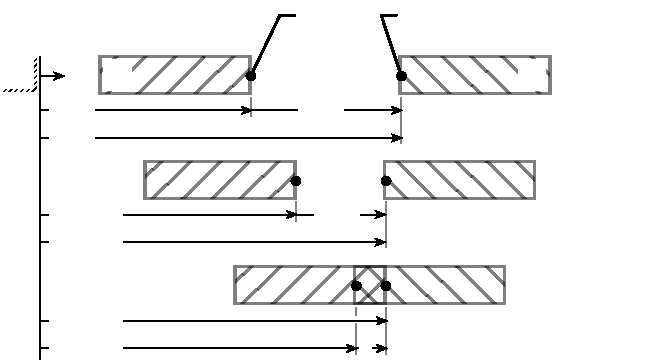
\includegraphics[width=0.9\textwidth]{fig/1D_contact}
%   %\includegraphics[width=3.5in]{../../AR/referenceFramesTwo.eps}
% \end{center}
% \caption{Caption to come.}
% \label{fig:1D_contact}
%\end{figure}

\begin{figure}[htb]
  \begin{center}
  %\begin{overpic}[width=\textwidth, grid, tics=10]{fig/1D_contact}
  \begin{overpic}[width=\textwidth]{fig/1D_contact}
  \put(17, 43.5){$\cA$}
  \put(81, 43.5){$\cB$}
  %
  \put(11, 43){$\vefa$}
  \put( 2, 43){$\cF$}
  %
  \put(48.5, 38){$g_0$}  
  \put(51.5, 22){$g$}    
  \put(56,  1){$p$}  
  %
  \put( 8, 47){$O$} 
  \put(46.5, 52.5){$P$}
  \put(62.5, 52.5){$Q$}
  %
  \put(88, 44){$t=t_0 = 0$}
  \put(88, 28){$t=t_1 > 0$}
  \put(88, 12){$t=t_2 = 3 t_1$}    
  %
  \put( 8.5, 38){$X^{OP}$}
  \put( 8.5, 33.5){$X^{OQ}$}    
  %
  \put( 8.5, 22){$\varphi^{OP}(t_1)$}
  \put( 8.5, 17.5){$\varphi^{OQ}(t_1)$}    
  %
  \put( 8.5,  5.5){$\varphi^{OP}(t_2)$}
  \put( 8.5,  1){$\varphi^{OQ}(t_2)$}      
 \end{overpic}
 \end{center}
 \caption{Caption to come.}
 \label{fig:1D_contact}
\end{figure}

At $t=0$, the initial gap $g_0 : [\Gamma_c \times 0] \mapsto \realplus$ 
between the two points $P$ and $Q$ is given by
\be
 g(t=0) = g_0 = X^{OQ} - X^{OP} \defe X^{PQ}, \hspace{1cm} g_0 > 0.
\ee
In general, the gap $g : [\Gamma_c \times \interval] \mapsto \real$ between the points is given by
\be
 g(\vvarphi(\vX), t) = \varphi^{OQ}_t - \varphi^{OP}_t = (X^{OQ} + u^Q_t) - (X^{OP} + u^P_t) = g_0 + u^Q_t - u^P_t,
\ee
where $u_t$ is a displacement, 
$\varphi_t$ is a current configuration, 
$\vu = \langle u^P_t, u^Q_t \rangle^T$, and
$\vvarphi = \langle \varphi^{OP}_t, \varphi^{OQ}_t \rangle^T$.
For arbitrary displacements $u^P_t$ and $u^Q_t$, the gap can be either positive, negative, or zero.
For example, at $t=t_2$, the gap is negative.  It is useful, as will seen in subsequent discussions on the penalty formulation ({\em see} ??), 
to define penetration $p$ as the negative of the gap.  
The penetration $p : [\Gamma_c \times \interval] \mapsto \real$ is defined as
\be
  p(\vu, t) \defe -g(\vu, t) = - \varphi^{OQ}_t + \varphi^{OP}_t = - (X^{OQ} + u^Q_t) + (X^{OP} + u^P_t) = - g_0 - u^Q_t + u^P_t.
\ee
Note that
\be
 p(t=0) = p_0 = - g_0, \hspace{1cm} p_0 < 0.
\ee

\subsubsection{Non-Penetration}
The penetration of body $\cA$ and body $\cB$, shown (for example) at $t=t_2$ in Fig.~\ref{fig:1D_contact}, is prevented
by constraining the gap $g$ (or, equivalently, the penetration $p$) as follows:
\begin{align}
 g &\geq 0, \\
 p &\leq 0.
\end{align}

Theses two inequality conditions are {\bf unilateral constraints} on the motion $\vvarphi$.  To illustrate
the unilateral constraint concept in a concrete sense, consider $\cB$ in Fig.~\ref{fig:1D_contact} to be 
stationary for all time.  Thus $u^Q_t = 0$, and we can abbreviate the displacement of body $\cA$ as 
$u^P_t = u$.  The gap and penetration functions are then
\begin{align}
 g(u) & = g_0 - u, \\
 p(u) & = -g(u) = u - g_0 = u + p_0.
\end{align}
Assume, for concreteness $g_0 = 1$~m.  The gap and penetration functions are then shown in
Fig.~\ref{fig:1D_gap_penetration}.

\begin{figure}[htb]
  \psfrag{a}{$(0, g_0)$}
  \psfrag{b}{$(g_0, 1)$}
  \psfrag{c}{$(-p_0, 0)$}
  \psfrag{d}{$(1, p_0)$}
  \psfrag{e}{$g(u) \geq 0$}
  \psfrag{f}{inadmissible}
  \psfrag{g}{inadmissible}
  \psfrag{h}{$p \leq 0$}
  \psfrag{s}{$\subset u \implies$ $g \geq 0$}
  \psfrag{t}{$\subset u \implies$ $p \leq 0$}    
  \begin{center}
   %\includegraphics[width=4.5in]{../AR/ARfinal.eps}
   %\includegraphics[width=4.5in]{../AR/AR_diagram_CBH.eps}
   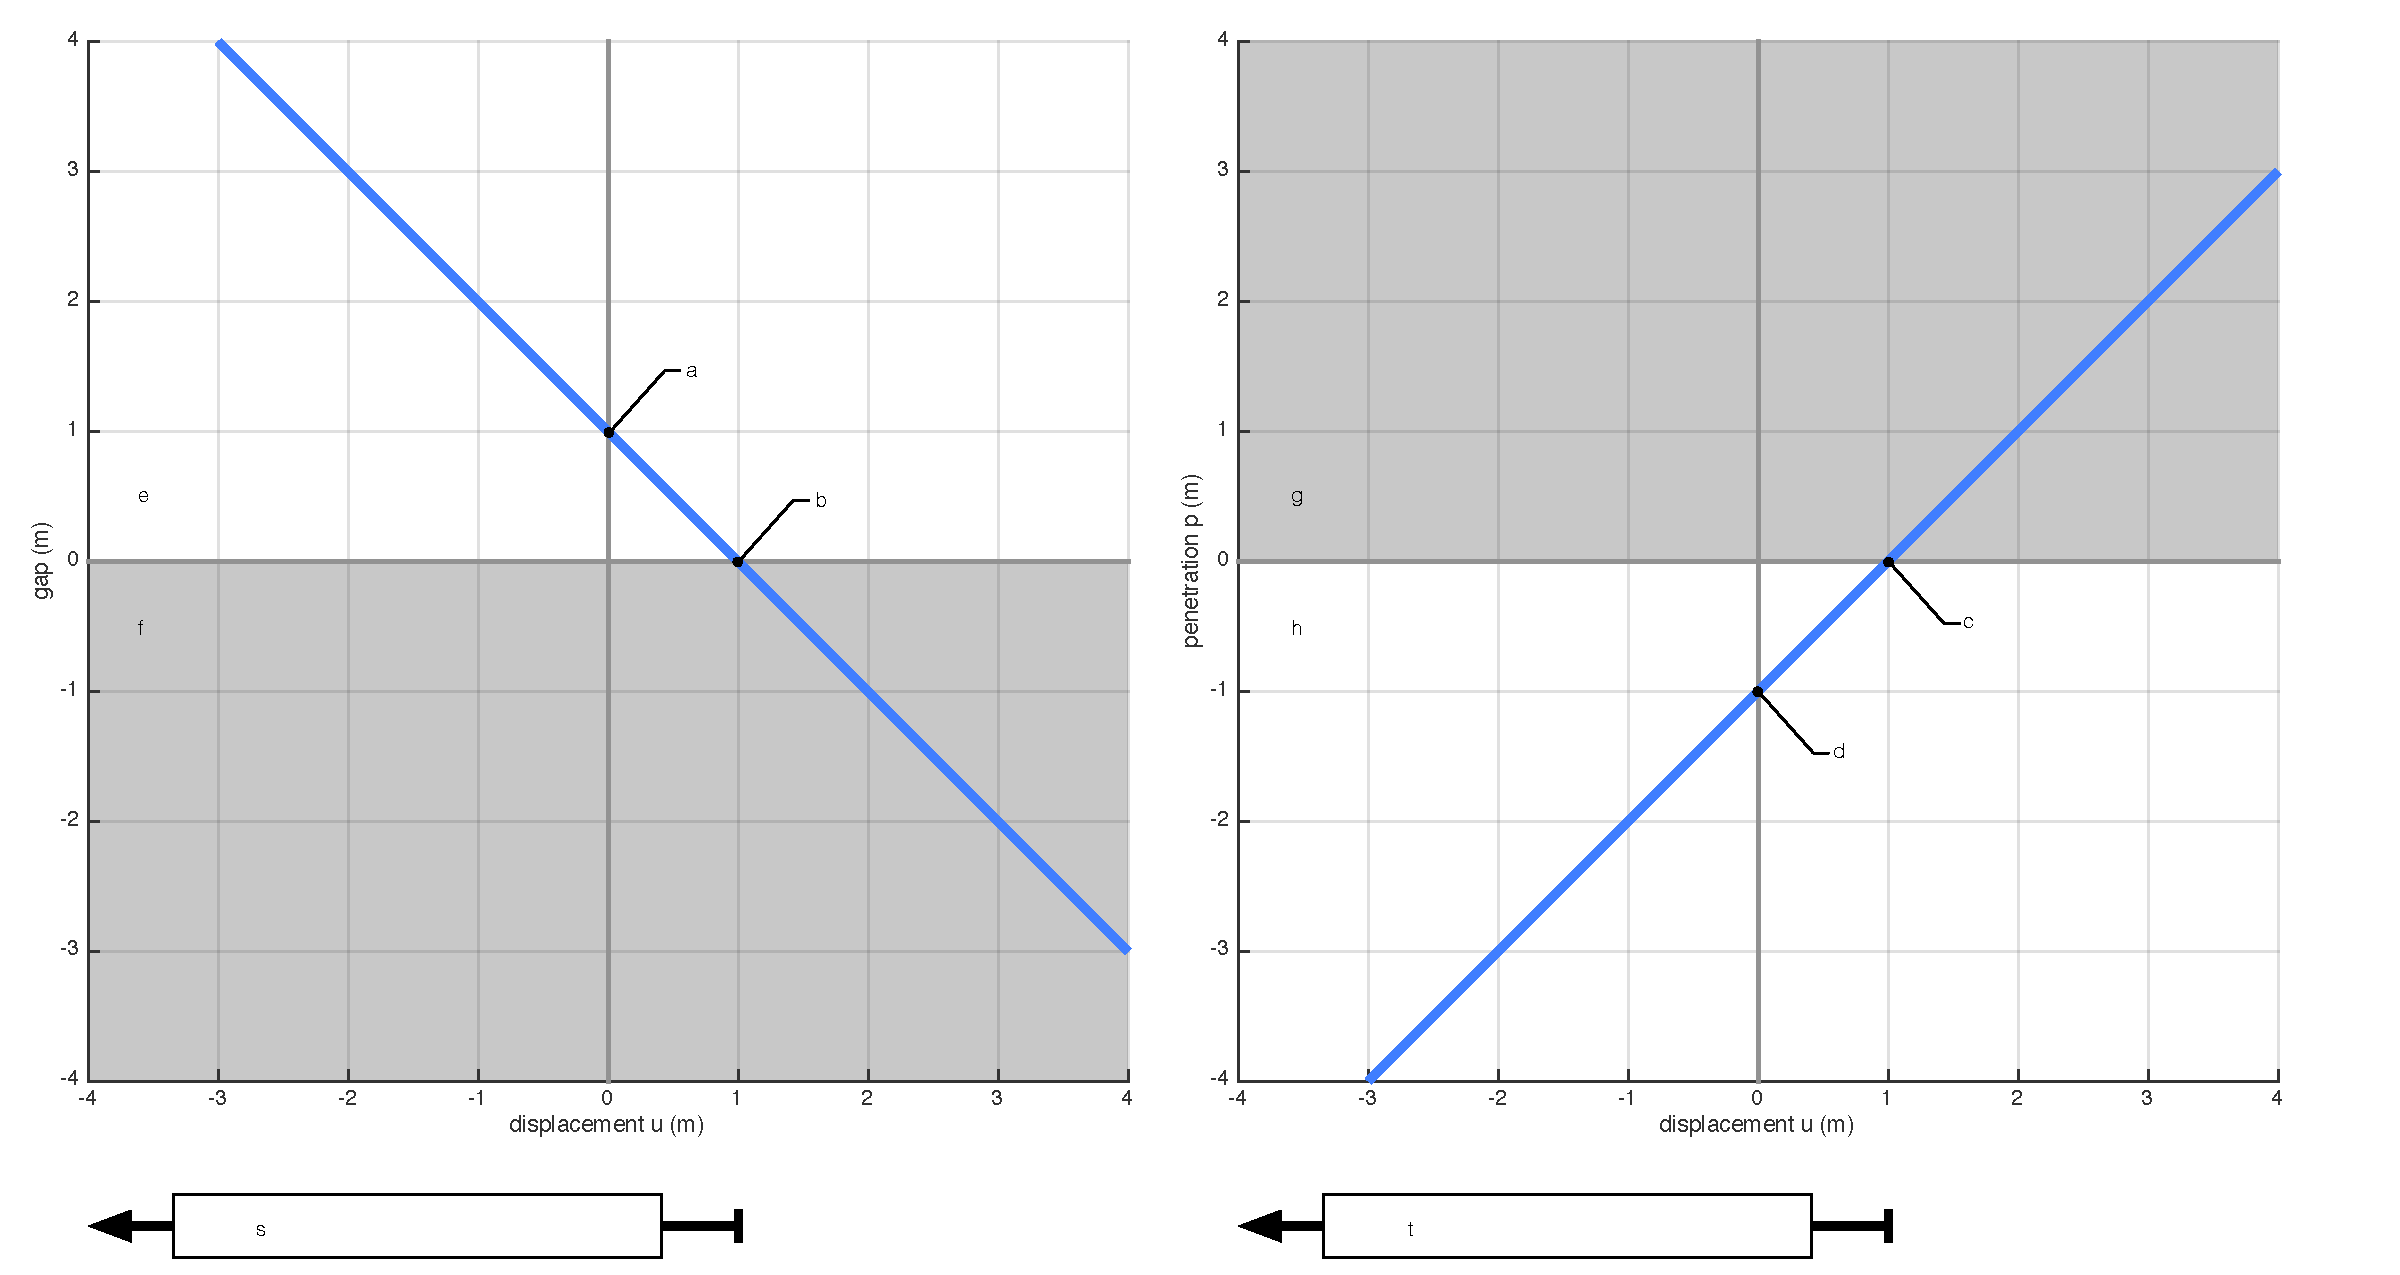
\includegraphics[width=\textwidth]{fig/1D_gap_penetration}
   %\includegraphics[width=3.5in]{../../AR/referenceFramesTwo.eps}
 \end{center}
 \caption{Caption to come.}
 \label{fig:1D_gap_penetration}
\end{figure}


\subsection{Example with Spring and Weight}
We start by considering a spring mass system, with spring constant $k$, mass $m$, gravitational field
$-g \; \vefb$, with the spring initially unstretched at $t=t_0 = 0$, as shown in Fig.~\ref{fig:1D_spring_mass}.  While this example does not yet have contact, it sets the context of energy minimization as method used to find static equilibrium.  

\begin{figure}[htb]
  \psfrag{0}{$0$} \psfrag{1}{$1$} 
  \psfrag{a}{$\vefa$}
  \psfrag{b}{$\vefb$}
  \psfrag{k}{$k$}    
  \psfrag{m}{$m g$} 
  \psfrag{n}{$-1$}       
  \psfrag{O}{$O$}
  \psfrag{R}{$t=t_0 = 0$}
  \psfrag{S}{$t=t_1 > 0$}
  \psfrag{X}{$X^{OP}$}
  \begin{center}
   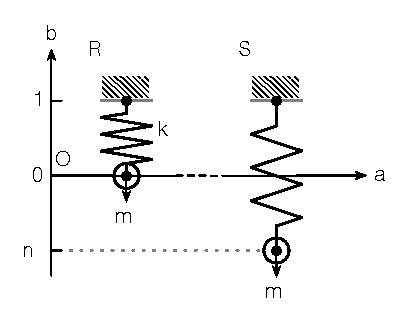
\includegraphics[width=0.5\textwidth]{fig/1D_spring_mass}
 \end{center}
 \caption{Caption to come.}
 \label{fig:1D_spring_mass}
\end{figure}

For concreteness, let $k=2$~N/m, $m=0.2$~kg, and $g=10$~m/s${^2}$, (for simplicity, rounded up from $9.81$~m/s${^2}$).  Let displacement $u$ of the mass, initially at $0$, be measured in the $\vefb$ axis.  
The internal energy (IE) of the spring as a function of $u$ is given by $\Pi_{k}(u) = \half k u^2$.
The potential energy (PE) of the mass as a function of $u$ is given by $\Pi_{m}(u) = m g u$.
Minimization of the potential energy gives
\begin{align}
 \delta \Pi = & \; \delta \left(\Pi_{k}(u) + \Pi_{m}(u) \right) = 
 \delta \left(\half k u^2 + m g u \right) = \left( k u + m g \right) \delta u \setequal 0, \\
 \implies u = & \; \frac{-m g}{k} = \frac{-0.2 \cdot 10}{2} = -1.
\end{align}

\begin{figure}[htb]
  \begin{center}
   %\includegraphics[width=4.5in]{../AR/ARfinal.eps}
   %\includegraphics[width=4.5in]{../AR/AR_diagram_CBH.eps}
   \includegraphics[width=0.8\textwidth]{fig/1D_spring_mass_plot_trim.eps}
   %\includegraphics[width=3.5in]{../../AR/referenceFramesTwo.eps}
 \end{center}
 \caption{Caption to come.}
 \label{fig:1D_spring_mass_plot}
\end{figure}

Fig.~\ref{fig:1D_spring_mass_plot} shows the spring internal energy, $\Pi_{k}(u)$, in dashed blue, which shows a minimum 
at $u=0$, and a symmetric, parabolic response for nonzero displacements, as expected.
The potential energy due to the mass, $\Pi_{m}(u)$, is shown in dot-dash green, which shows a linear relationship in $u$ with intercept $0$ and slope $m g = 0.2 \cdot 10 = 2$~N.

The addition of the two aforementioned potentials, $\Pi(u) = \Pi_{k}(u) + \Pi_{m}(u)$, is shown in solid red.
The system potential, $\Pi(u)$, has a minimum at $u=-1$~m, as expected.
Next, we used this concept of minimizing potential energy in the context of contact.

\subsection{Example with Spring and Rigid Wall}
Consider a spring, shown in Fig.~\ref{fig:1D_spring_wall}, with elastic constant $k = 2$~N/m, undeformed length $L_0 = 2$~m subjected to a prescribed displacement in the amount of $\bar{u} = 2$~m on the left-hand-side.\footnote{This example follows Laursen TA (2013), {\em Computational contact and impact mechanics: fundamentals of modeling interfacial phenomena in nonlinear finite element analysis.} Springer Science \& Business Media, page 87.}
A rigid wall is $g_0 = X^{PQ} = 1$~m from the right-hand-side of the spring at $t=0$.
At $t=t_1$, the spring has undergone its prescribed displacement and penetrates the wall by amount $p$.  
In this configuration, internal energy $\Pi$ for the spring for the as a function of $u = u^P$ is given by
\be
 \Pi(u) = \frac{1}{2} \; k \; \delta^2 = \frac{1}{2} \; 2 \; (u - \bar{u})^2 = (u - 2)^2 \; (\mbox{Nm}).
\ee

\begin{figure}[htb]
  \psfrag{0}{$0$} \psfrag{1}{$1$} \psfrag{2}{$2$} \psfrag{3}{$3$} \psfrag{4}{$4$}
  \psfrag{A}{$\cA$}
  \psfrag{a}{$\vefa$}
  \psfrag{B}{$\cB$}  
  \psfrag{c}{$\bar{u}$}
  \psfrag{d}{$\bar{u}=2$}
  \psfrag{F}{$\cF$}
  \psfrag{G}{$g_0$}  
  \psfrag{g}{$g$}    
  \psfrag{k}{$k$}      
  \psfrag{O}{$O$}
  \psfrag{P}{$P$}
  \psfrag{p}{$p$}  
  \psfrag{Q}{$Q$}
  \psfrag{R}{$t=t_0 = 0$}
  \psfrag{S}{$t=t_1 > 0$}
  \psfrag{T}{$t=t_2 > t_1$}    
  \psfrag{X}{$X^{OP}$}
  \psfrag{x}{$\varphi^{OP}(t_1)$}
  \psfrag{u}{$\varphi^{OP}(t_2)$}
  \psfrag{Y}{$X^{OQ}$}    
  \psfrag{y}{$\varphi^{OQ}(t_1)$}    
  \psfrag{v}{$\varphi^{OQ}(t_2)$}      
  \begin{center}
   %\includegraphics[width=4.5in]{../AR/ARfinal.eps}
   %\includegraphics[width=4.5in]{../AR/AR_diagram_CBH.eps}
   \includegraphics[width=0.5\textwidth]{fig/1D_spring_wall.eps}
   %\includegraphics[width=3.5in]{../../AR/referenceFramesTwo.eps}
 \end{center}
 \caption{Caption to come.}
 \label{fig:1D_spring_wall}
\end{figure}





\subsubsection{Principle of Minimum Potential Energy}
\subsubsection{Principle of Minimum Potential Energy with Lagrange Multiplier Enforcement}


\begin{figure}[htb]
  \psfrag{t}{$\subset u \implies$ $p \leq 0$}    
  \begin{center}
   %\includegraphics[width=4.5in]{../AR/ARfinal.eps}
   %\includegraphics[width=4.5in]{../AR/AR_diagram_CBH.eps}
   \includegraphics[width=0.8\textwidth]{fig/1D_spring_with_wall_trim_soln.eps}
   %\includegraphics[width=3.5in]{../../AR/referenceFramesTwo.eps}
 \end{center}
 \caption{Caption to come.}
 \label{fig:1D_spring_with_wall_soln}
\end{figure}

\clearpage

\begin{figure}[htb]
  \psfrag{a}{$\lambda = 0$}
  \psfrag{b}{$\lambda = \half$}  
  \psfrag{c}{$\lambda = 1$}
  \psfrag{d}{$\lambda = 2$}
  \psfrag{e}{$\lambda = 3$}
  \psfrag{f}{$\lambda = 4$}  
  \psfrag{g}{$\lambda = 5$}    
  \psfrag{h}{$\lambda = 6$}      
  \psfrag{t}{$\subset u \implies$ $p \leq 0$}    
  \begin{center}
   %\includegraphics[width=4.5in]{../AR/ARfinal.eps}
   %\includegraphics[width=4.5in]{../AR/AR_diagram_CBH.eps}
   \includegraphics[width=\textwidth]{fig/1D_spring_with_wall_new_trim.eps}
   %\includegraphics[width=3.5in]{../../AR/referenceFramesTwo.eps}
 \end{center}
 \caption{Caption to come.}
 \label{fig:1D_spring_with_wall}
\end{figure}

\begin{align}
 \Pi(u) & = \Pi_k(u) + \Pi_c(u). \\
 & = \half k \left(u - \bar{u}\right)^2 + \lambda p(u). \\
 & = \left(u - \bar{u}\right)^2 + \lambda (u + p_0). \\
 & \mbox{where} \; \bar{u} = 2~\mbox{m}, \; \mbox{and} \; p_0 = -1~\mbox{m}.
\end{align}


\begin{figure}[htb]
  \psfrag{a}{(a)}
  \psfrag{b}{(b)}
  \psfrag{c}{(c)}
  \psfrag{d}{(d)}
  \begin{center}
   \includegraphics[width=\textwidth]{fig/1D_spring_with_wall_iso_trim.eps}
 \end{center}
 \caption{Caption to come.}
 \label{fig:1D_spring_with_wall_iso}
\end{figure}


\subsubsection{Principle of Minimum Potential Energy with Penalty Enforcement}
\subsubsection{Principle of Minimum Potential Energy with Augmented Lagrange Multiplier Enforcement}



%====================
%\pagebreak
%\appendix
%\section{Numerical Details}
%====================


\end{document}








  \section{Shock}

\subsection{Introduction}

\subsection{An Ideal Fluid}

\subsection{Definition of a Shock}

\subsection{Conservation Laws for a Single Shock}
\subsubsection{Laboratory Fixed Coordinate Frame}
The derivation that follows assumes a {\bf laboratory-fixed reference
frame}, as shown in Fig.~\ref{fig:piston_shock_cv}.\footnote{A shock-fixed 
reference frame derivation then is developed in a subsequent section.}
Consider a rigid tube containing a rigid piston material at ambient
density $\rho_0$ and ambient pressure $P_0$ at time $t=t_0$.  

\begin{figure}[htb]
  \begin{center}
  %\begin{overpic}[width=\textwidth, grid, tics=10]{fig/piston_shock_cv}
  \begin{overpic}[width=\textwidth]{fig/piston_shock_cv}
    \put(14, 29){$O$}
    \put(95, 31){$x$}
    \put(15, 38){$y$}
    \put(12, 27){$z$}
    \put(23,  9.5){$U_P \cdot \Delta t$}
    \put(49,  9.5){$(U_P - U_P) \cdot \Delta t$}
    \put(44,  3.5){$U_S \cdot \Delta t$}
    \put( 2, 47){\footnotesize piston at time $t=t_0$}
    \put(28, 47){\footnotesize piston at time $t=(t_0 + \Delta t)$}
    \put(58, 47){\footnotesize shock with speed $U_S$ at $t=(t_0 + \Delta t)$}
    \put(49, 30){$\rho_1, P_1, U_P$}
    \put(85, 30){$\rho_0, P_0$}
  \end{overpic}
  \end{center}
  \caption{Piston moving left-to-right along the $x$-axis, with 
  piston speed $U_P$, causing shock with shock speed $U_S$.}
  \label{fig:piston_shock_cv}
\end{figure}

Assume at time $t=t_0 + \Delta t$, the piston moves left-to-right
along the $x$-axis with speed $U_P$, measured in the fixed 
laboratory reference frame.  
Assume the piston speed $U_P$ causes a shock to propagate through
the material with speed $U_S$.  We require the following:
\begin{itemize}
  \item $0 < U_P < +\infty$
  \item $0 < U_S < +\infty$
  \item $U_P < U_S$
\end{itemize}  
From these considerations, we conclude that the material to the left of the
shock wave in Fig.~\ref{fig:piston_shock_cv} moves to the right at speed
$U_S$.  The material to the right of the shock wave remains at 
rest.\footnote{Furthermore, we assume the material throughout the tube and
for all time is inviscid, non-diffusive, and non-reacting.  We assume 
an adiabatic boundary, thus no
heat conduction occurs through the boundary of the tube walls or piston.
We assume no heat transfer from radiation occurs across the shock.  Finally, 
we assume body forces from gravity and electromagnetism are negligible.}

Since the piston compresses the material in the tube, we know
\begin{itemize}
\item $\rho_0 < \rho_1$.
\end{itemize}

Allow some time interval $\Delta t$ to elapse, as illustrated 
in Fig.~\ref{fig:piston_shock_cv}.  Consider the distances along the
$x$-axis, written as a multiplication of speeds and elapsed time.  
In the time interval $\Delta t$, the piston moves along the $x$-axis
a distance of $U_P \cdot \Delta t$.  
In the same time interval, the shock wave moves along the $x$-axis
a distance of $U_S \cdot \Delta t$.  Thus, the control volume at 
$t=(t_0 + \Delta t)$ has an axial length of $(U_S - U_P) \cdot \Delta t$.

From these axial lengths and piston cross-sectional area $A$, we can write
the following relationships:

\begin{itemize}
\item volume
\begin{itemize}
%
\item[] $V_0 = \left.V\right|_{t=t_0} = A \cdot U_S \cdot \Delta t$,
\item[] $V_1 = \left.V\right|_{t=(t_0 + \Delta t)} = A \cdot \left(
U_S - U_P\right) \cdot \Delta t$,
\end{itemize}
%
\item density
\begin{itemize}
\item[] $\rho_0 = \left.\rho\right|_{t=t_0}$,
\item[] $\rho_1 = \left.\rho\right|_{t=(t_0 + \Delta t)}$,
\end{itemize}
%
\item mass 
\begin{itemize}
\item[] $\rho_0 V_0 = \rho_0 \cdot A \cdot U_S \cdot \Delta t$, 
\item[] $\rho_1 V_1 = \rho_1 \cdot A \cdot \left(U_S - U_P\right) \cdot 
\Delta t$.
\end{itemize}
%
\end{itemize}

\subsubsection{Conservation of Mass}
Conservation of mass within the control volume requires that mass at
time $t=(t_0 + \Delta t)$ be unchanged from mass at time $t=t_0$.  
Thus
\be
 \rho_0 \cdot A \cdot U_S \cdot \Delta t =
 \rho_1 \cdot A \cdot \left(U_S - U_P\right) \cdot \Delta t, 
\ee
or
\be
 \boxed{\rho_0 U_S = \rho_1 \left(U_S - U_P\right).}
\ee

\subsubsection{Conservation of Momentum}
The driving force from the piston on the material is $(P_1 - P_0) \cdot A$.
Conservation of momentum requires $F = d(ma)/dt$.  Written over the time
interval $\Delta t$ and for constant mass, 
conservation of momentum can be written
\be
 F \cdot \Delta t = m \cdot \Delta U.
\ee
Rewriting this expression in terms of pressures and densities, we have
\be(P_1 - P_0) \cdot A \cdot \Delta t = \left(\rho_0 \cdot A \cdot U_S \cdot 
\Delta T \right) \; \left(U_P - 0\right) 
\ee
which gives
\be
\boxed{P_1 - P_0  = \rho_0 \; U_S \; U_P.}
\label{eq:cons_momentum}
\ee

\subsubsection{Conservation of Energy}
The work done on the control volume by the piston moving left-to-right
is given by
\be
W_P = \underset{\mbox{\footnotesize force}}{\underbrace{P_1 \cdot A}}
\cdot 
 \underset{\mbox{\footnotesize disp.}}{\underbrace{U_P \cdot \Delta t}}.
\ee
The kinetic energy increase of the control volume is simply the one-half times
the mass times the square of the change in velocity, thus
\be
KE = \half  \;
\underset{\mbox{\footnotesize mass}}{\underbrace{\left(\rho_0 \cdot A 
\cdot U_S \cdot \Delta t\right)}} \;
\underset{\mbox{\footnotesize velocity}}{\underbrace{\left(U_P - 0
\right)}}^2.
\ee
Finally, the increase in internal energy is just the internal energy 
{\bf per unit mass}, $e$, multiplied by the mass, 
\be
IE = (e_1 - e_0)  \;
\underset{\mbox{\footnotesize mass}}{\underbrace{\left(\rho_0
 \cdot A \cdot U_S \cdot \Delta t\right)}}.
\ee
Equating these quantities gives
\be
P_1 \cdot A \cdot U_P \cdot \Delta t = 
\half \; \rho_0 \cdot A \cdot U_S \cdot \Delta t \cdot U_P^2 + 
\left(e_1 - e_0\right) \; \rho_0 \cdot A \cdot U_S \cdot \Delta t
\ee
or simply
\be
\boxed{P_1 \; U_P = \rho_0 \; U_S \left(\frac{U_P^2}{2} + e_1 - e_0\right).}
\label{eq:cons_energy}
\ee
The foregoing equation can be written without kinematic variables 
$U_S$ and $U_P$. Define the specific volume as
\be
V \defe \frac{1}{\rho}.
\label{eq:specific_volume}
\ee
Next, note that conservation of mass can be rewritten as 
\be
\frac{U_P}{U_S} = 1 - \frac{\rho_0}{\rho_1}.
\label{eq:cons_mass_ratio}
\ee
Then, with (\ref{eq:cons_energy}),
\begin{align}
P_1 \; U_P 
&\overset{(\ref{eq:cons_momentum})}{=} 
\left(P_1 - P_0\right) \frac{U_P}{2} + \rho_0 \; U_S \; (e_1 - e_0), \\
&= -P_0 \; U_P + 2 \; \rho_0 \; U_S \; (e_1 - e_0), \\
(e_1 - e_0) &= \frac{U_P \; (P_1 + P_0)}{2 \; \rho_0 \; U_S}, \\
&\overset{(\ref{eq:cons_mass_ratio})}{=} 
\left(\frac{P_1 + P_0}{2\;\rho_0}\right) \; 
\left(1 - \frac{\rho_0}{\rho_1}\right), \\
&\overset{(\ref{eq:specific_volume})}{=} 
\left(\frac{P_1 + P_0}{2}\right) V_0 \left(1 - \frac{V_1}{V_0}\right), 
\end{align}
which simplifies to
\be
\boxed{e_1 - e_0 = \left(\frac{P_1 + P_1}{2}\right) \; (V_0 - V_1).}
\ee

\subsubsection{Alternative Formulations}
Now we develop the {shock-fixed reference frame} equations for mass, 
momentum, and energy conservation.


%

\chapter{Implementation}

\begin{figure}[htb]
  \begin{center}
    %\begin{overpic}[width=\textwidth, grid, tics=10]{fig/iso_geo_001}
    %\begin{overpic}[width=\textwidth,natwidth=608,natheight=788]{fig/iso_geo_001.pdf}
    \begin{overpic}[width=\textwidth]{fig/iso_geo_001.pdf}
      %
    \end{overpic}
  \end{center}
  \caption{Isogeometric analysis page 1.}
  \label{fig:iso_geo_001} % label must come after caption 
\end{figure}

\begin{figure}[htb]
  \begin{center}
    %\begin{overpic}[width=\textwidth, grid, tics=10]{fig/iso_geo_002}
    \begin{overpic}[width=\textwidth]{fig/iso_geo_002.pdf}
      %
    \end{overpic}
  \end{center}
  \caption{Isogeometric analysis page 2.}
  \label{fig:iso_geo_002} % label must come after caption 
\end{figure}

\begin{figure}[htb]
  \begin{center}
    %\begin{overpic}[width=\textwidth, grid, tics=10]{fig/iso_geo_003}
    \begin{overpic}[width=\textwidth]{fig/iso_geo_003.pdf}
      %
    \end{overpic}
  \end{center}
  \caption{Isogeometric analysis page 3.}
  \label{fig:iso_geo_003}% label must come after caption 
\end{figure}

\begin{figure}[htb]
  \begin{center}
    %\begin{overpic}[width=\textwidth, grid, tics=10]{fig/iso_geo_004}
    \begin{overpic}[width=\textwidth]{fig/iso_geo_004.pdf}
      %
    \end{overpic}
  \end{center}
  \caption{Isogeometric analysis page 4.}
  \label{fig:iso_geo_004}% label must come after caption 
\end{figure}


%  
\section{Finite Elements}

\subsection{Lines}

\subsubsection{LL2}
The linear two-noded line finite element has shape functions 
with the general form $\phi(\xi) = A + B \xi$.
\begin{figure}[htb]
  \begin{center}
    %\begin{overpic}[width=0.5\textwidth, grid, tics=10]{fig/LL2}
    %\begin{overpic}[width=0.5\textwidth,natwidth=360,natheight=108]{fig/LL2.pdf}
    \begin{overpic}[width=0.5\textwidth]{fig/LL2.pdf}
      \put(85, 22){$\xi$}
      \put(44, 25){$\xi=0$}
      %
      \put(18.5, 10){\bf 1}
      \put(17,  3){\footnotesize(-1)}
      %
      \put(78.5, 10){\bf 2}
      \put(77,  3){\footnotesize(1)}
    \end{overpic}
  \end{center}
  \caption{Linear two-noded line finite element.}
  \label{fig:LL2} % label must come after caption
\end{figure}

\begin{align}
 \phi_1(\xi) & = \;-\frac{1}{2} 
                 \hspace{0.65cm}
		 \cdot 
		 \hspace{0.65cm}
		 \left( \xi - 1 \right) \\
 \phi_2(\xi) & = \hspace{0.45cm} \frac{1}{2}
                 \;\left( \xi + 1 \right)
		 \hspace{0.65cm}
		 \cdot
\end{align}

\begin{Hremark}
\label{remark:node_connotation}
Note that 
``$\;\;\cdot$\;\;'' 
as used here has a dual purpose.  First, it denotes multiplication, and
by this measure alone, is unnecessary to include.  However, the second
purpose is a connotation of location, from left-to-right on the $\xi$-axis, 
where the shape function must be unity.  Moreover, the quantities in
parentheses 
(~\hspace{0.4cm}~) 
connote where the shape function must go to zero.  
\end{Hremark}

\clearpage
\subsubsection{LL3}
The linear three-noded line finite element has shape functions 
with the general form $\phi(\xi) = A + B \xi + C \xi^2$.
\begin{figure}[htb]
  \begin{center}
    %\begin{overpic}[width=0.5\textwidth, grid, tics=10]{fig/LL3}
    %\begin{overpic}[width=0.5\textwidth,natwidth=360,natheight=108]{fig/LL3.pdf}
    \begin{overpic}[width=0.5\textwidth]{fig/LL3.pdf}
      \put(85, 22){$\xi$}
      \put(44, 25){$\xi=0$}
      %
      \put(18.5, 10){\bf 1}
      \put(17,  3){\footnotesize(-1)}
      %
      \put(48.5, 10){\bf 2}
      \put(47.25,  3){\footnotesize(0)}
      %
      \put(78.5, 10){\bf 3}
      \put(77,  3){\footnotesize(1)}
    \end{overpic}
  \end{center}
  \caption{Linear three-noded line finite element.}
  \label{fig:LL3} % label must come after caption
\end{figure}

\begin{align}
 \phi_1(\xi) & = \;\;\frac{1}{2} 
                 \hspace{0.65cm}
		 \cdot 
		 \hspace{0.8cm}
                 \left( \xi  \right)
		 \;\;\left( \xi - 1 \right) \\
 \phi_2(\xi) & = -1 \;
                 \left( \xi + 1 \right)
		 \hspace{0.42cm}
		 \cdot
		 \hspace{0.42cm} 
		 \left( \xi - 1 \right) \\
 \phi_3(\xi) & = \;\;\frac{1}{2} \;
                 \left( \xi + 1 \right)
		 \;\;\;\left( \xi  \right)
		 \hspace{0.7cm}
		 \cdot
\end{align}
See Remark~\ref{remark:node_connotation} for an explanation of the 
multiplication 
``$\;\;\cdot$\;\;'' 
and parentheses (~\hspace{0.4cm}~) notation.



\clearpage
\subsubsection{LL4}
The linear four-noded line finite element has shape functions 
with the general form $\phi(\xi) = A + B \xi + C \xi^2 + D \xi^3$.
\begin{figure}[htb]
  \begin{center}
    %\begin{overpic}[width=0.5\textwidth, grid, tics=10]{fig/LL4}
    %\begin{overpic}[width=0.5\textwidth,natwidth=360,natheight=108]{fig/LL4.pdf}
    \begin{overpic}[width=0.5\textwidth]{fig/LL4.pdf}
      \put(85, 22){$\xi$}
      \put(44, 25){$\xi=0$}
      %
      \put(18.5, 10){\bf 1}
      \put(17,  3){\footnotesize(-1)}
      %
      \put(38.5, 10){\bf 2}
      \put(35,  3){\footnotesize$\left(-\frac{1}{3}\right)$}
      %
      \put(58.5, 10){\bf 3}
      \put(56.5,  3){\footnotesize$\left(\frac{1}{3}\right)$}
      %
      \put(78.5, 10){\bf 4}
      \put(77,  3){\footnotesize(1)}
    \end{overpic}
  \end{center}
  \caption{Linear four-noded line finite element.}
  \label{fig:LL4} % label must come after caption
\end{figure}

\begin{align}
 \phi_1(\xi) & = \frac{-9}{16} 
                 \hspace{0.5cm}
		 \cdot 
		 \hspace{0.5cm}
                 \left( \xi + \frac{1}{3} \right)
                 \left( \xi - \frac{1}{3} \right) 
		 \left( \xi - 1 \right) \\
 \phi_2(\xi) & = \frac{9}{16} \;
                 \left( \xi + 1 \right)
		 \hspace{0.7cm}
		 \cdot
		 \hspace{0.7cm} 
		 \left( \xi - \frac{1}{3} \right) 
		 \left( \xi - 1 \right) \\
 \phi_3(\xi) & = \frac{-9}{16} 
                 \left( \xi + 1 \right)
		 \left( \xi + \frac{1}{3} \right)
		 \hspace{0.7cm}
		 \cdot
		 \hspace{0.7cm}
		 \left( \xi - 1 \right) \\
 \phi_4(\xi) & = \frac{9}{16} \;
                 \left( \xi + 1 \right)
		 \left( \xi + \frac{1}{3} \right)
		 \left( \xi - \frac{1}{3} \right)
		 \hspace{0.5cm}
		 \cdot
\end{align}
See Remark~\ref{remark:node_connotation} for an explanation of the 
multiplication 
``$\;\;\cdot$\;\;'' 
and parentheses (~\hspace{0.4cm}~) notation.


\clearpage
\subsection{Triangles}

\subsubsection{LT3}
The linear three-noded triangular finite element has shape functions 
with the general form $\phi(\vxi) = A + B \xi_1 + C \xi_2$.
\begin{figure}[htb]
  \begin{center}
    %\begin{overpic}[width=0.5\textwidth, grid, tics=10]{fig/LT3}
    %\begin{overpic}[width=0.5\textwidth,natwidth=360,natheight=360]{fig/LT3.pdf}
    \begin{overpic}[width=0.5\textwidth]{fig/LT3.pdf}
      \put(85, 20){$\xi_1$}
      \put(20, 85){$\xi_2$}
      %
      \put( 8,  8){\bf 3}
      \put( 4,  3){\footnotesize(0, 0)}
      %
      \put(80,  8){\bf 1}
      \put(76,  3){\footnotesize(1, 0)}
      %
      \put( 8, 80){\bf 2}
      \put( 4, 75){\footnotesize(0, 1)}
    \end{overpic}
  \end{center}
  \caption{Linear three-noded triangular finite element.}
  \label{fig:LT3} % label must come after caption
\end{figure}

\begin{align}
 \phi_1(\vxi) & = \xi_1 \\
 \phi_2(\vxi) & = \xi_2 \\
 \phi_3(\vxi) & = 1 - \xi_1 - \xi_2 
\end{align}

\clearpage
\subsubsection{LT6}
The linear six-noded triangular finite element has shape functions 
with the general form $\phi(\vxi) = A + B \xi_1 + C \xi_2 + D \xi_1 \xi_2
 + E \xi_1^2 \xi_2 + F \xi_1 \xi_2^2.$
\begin{figure}[htb]
  \begin{center}
    %\begin{overpic}[width=0.5\textwidth, grid, tics=10]{fig/LT6}
    %\begin{overpic}[width=0.5\textwidth,natwidth=360,natheight=360]{fig/LT6.pdf}
    \begin{overpic}[width=0.5\textwidth]{fig/LT6.pdf}
      \put(85, 20){$\xi_1$}
      \put(20, 85){$\xi_2$}
      %
      \put( 8,  8){\bf 3}
      \put( 4,  3){\footnotesize(0, 0)}
      %
      \put(80,  8){\bf 1}
      \put(76,  3){\footnotesize(1, 0)}
      %
      \put( 8, 80){\bf 2}
      \put( 4, 75){\footnotesize(0, 1)}
      %
      \put(55, 55){\bf 4}
      \put(50, 50){\footnotesize($\half$, $\half$)}
      %
      \put( 8, 45){\bf 5}
      \put( 4, 40){\footnotesize(0, $\half$)}
      %
      \put(46,  8){\bf 6}
      \put(42,  3){\footnotesize($\half$, 0)}
    \end{overpic}
  \end{center}
  \caption{Linear six-noded triangular finite element.}
  \label{fig:LT6} % label must come after caption
\end{figure}

\begin{align}
 \phi_1(\vxi) & = 2 \; \xi_1 \left(\xi_1 - \half \right) \\
 \phi_2(\vxi) & = 2 \; \xi_2 \left(\xi_2 - \half \right) \\
 \phi_3(\vxi) & = 2 \left( 1 - \xi_1 - \xi_2 \right) 
                  \left( \half - \xi_1 - \xi_2 \right) \\
 \phi_4(\vxi) & = 4 \; \xi_1 \; \xi_2 \\
 \phi_5(\vxi) & = 4 \left(1 - \xi_1 - \xi_2\right) \xi_2 \\
 \phi_6(\vxi) & = 4 \left(1 - \xi_1 - \xi_2\right) \xi_1
\end{align}

\clearpage
\subsubsection{LT6 Detailed Derivation}

\begin{figure}[htb]
  \begin{center}
    %\begin{overpic}[width=\textwidth, grid, tics=10]{fig/LT6_explicated}
    %\begin{overpic}[width=\textwidth,natwidth=684,natheight=360]{fig/LT6_explicated.pdf}
    \begin{overpic}[width=\textwidth]{fig/LT6_explicated.pdf}
      \put(50, 10){$\xi_1$}
      \put(96, 10){$\xi_1$}
      \put(10, 49){$\xi_2$}
      \put(57, 49){$\xi_2$}
      %
      \put(9.5,  2){$H_1$}
      \put(60,  2){$H_2$}
      %
      \put( 2, 32.5){$V_1$}
      \put(82, 26){$V_2$}
      %
      \put(25.3, 44.8){$D_1$}
      \put(70, 41){$D_2$}
    \end{overpic}
  \end{center}
  \caption{Detailed derivation of the linear 
  six-noded triangular finite element, with horizontal lines $H_1$ and 
  $H_2$, vertical lines $V_1$ and $V_2$, and diagonal lines $D_1$ and 
  $D_2$.}
  \label{fig:LT6_explicated} % label must come after caption
\end{figure}

We begin by writing equations of two horizontal, two vertical, and
two diagonal lines, as outlined in Fig.~(\ref{fig:LT6_explicated}).
\begin{align}
 H_1 & : \xi_2 = 0 \;\;\;\forall\;\;\; \xi_1 \\
 H_2 & : \xi_2 = \half \;\;\forall\;\;\; \xi_1  
         \implies 0 = \left( \xi_2 - \half \right) \\
 V_1 & : \xi_1 = 0 \;\;\;\forall\;\;\; \xi_2 \\
 V_2 & : \xi_1 = \half \;\;\forall\;\;\; \xi_2 
         \implies 0 = \left( \xi_1 - \half \right) \\
 D_1 & : \xi_2 = 1 - \xi_1 \;\;\;
         \implies 0 = \left( 1 - \xi_1 - \xi_2 \right) \\
 D_2 & : \xi_2 = \half - \xi_1 \;\;
         \implies 0 = \left( \half - \xi_1 - \xi_2 \right)
\end{align}
These six equations represent lines where the shape function has zero
value for all combinations of $(\xi_1, \xi_2)$.  Using these lines, 
we can construct shape functions as a functional products of $(\xi_1, \xi_2$)
and locations (e.g., lines that intersect nodes) where the nodal
values of the shape function must be identically zero.  

Let shape function $\phi_1$ have coefficient $A_1$.  Then $\phi_1$ can be
written as 
\be
\phi_1(\vxi) = A_1 \cdot V_1 \cdot V_2 = A_1 \cdot \xi_1 \cdot
\left(\xi_1 - \half \right).
\ee
Then, evaluating $\phi_1$ at the node {\bf 1} location gives
\be
\phi_1(1,0) = A_1 (1) \left( \half \right) \overset{\mbox{\tiny set}}{=} 1
\implies A_1 = 2.
\ee
The form of $\phi_2$ follows similarly to $\phi_1$.
Next, consider $\phi_3$.
\be 
\phi_3(\vxi) = A_3 \cdot D_1 \cdot D_2 = A_3 \cdot \left( \half 
- \xi_1 - \xi_2 \right) \cdot \left( 1 - \xi_1 - \xi_2 \right).
\ee
Then, evaluating $\phi_3$ at the node {\bf 3} location gives
\be
\phi_3(0,0) = A_3 \left( \half \right) (1) \overset{\mbox{\tiny set}}{=} 1
\implies A_3 = 2.
\ee
Finally, $\phi_4$, $\phi_5$ and $\phi_6$ can be found readily (we omit
some details now that the pattern has been shown above)
as
\begin{align}
\phi_4 & = A_4 \cdot H_1 \cdot V_1 \;\;\;\;\mbox{and}\;\;\; A_4 = 4, \\
\phi_5 & = A_5 \cdot H_1 \cdot D_1 \;\;\;\mbox{and}\;\;\; A_5 = 4, \\
\phi_6 & = A_6 \cdot V_1 \cdot D_1 \;\;\;\;\mbox{and}\;\;\; A_6 = 4. 
\end{align}



\clearpage
\subsubsection{LT10}
The linear ten-noded triangular finite element has shape functions 
with the general form $\phi(\vxi) = A + B \xi_1 + C \xi_2 + D \xi_1 \xi_2
 + E \xi_1^2 + F \xi_2^2 + G \xi_1^2 \xi_2 + H \xi_1 \xi_2^2 + I \xi_1^3
 + J \xi_2^3$.
\begin{figure}[htb]
  \begin{center}
    %\begin{overpic}[width=0.5\textwidth, grid, tics=10]{fig/LT10}
    %\begin{overpic}[width=0.5\textwidth,natwidth=360,natheight=360]{fig/LT10.pdf}
    \begin{overpic}[width=0.5\textwidth]{fig/LT10.pdf}
      \put(85, 20){$\xi_1$}
      \put(20, 85){$\xi_2$}
      %
      \put( 8,  8){\bf 3}
      \put( 4,  3){\footnotesize(0, 0)}
      %
      \put(80,  8){\bf 1}
      \put(76,  3){\footnotesize(1, 0)}
      %
      \put( 8, 80){\bf 2}
      \put( 4, 75){\footnotesize(0, 1)}
      %
      \put( 8, 55){\bf 6}
      \put( 4, 50){\footnotesize(0, $\frac{2}{3}$)}
      %
      \put( 8, 35){\bf 7}
      \put( 4, 30){\footnotesize(0, $\frac{1}{3}$)}
      %
      \put(38, 38){\bf 10}
      \put(38, 29){\footnotesize($\frac{1}{3}$, $\frac{1}{3}$)}
      % 
      \put(58, 38){\bf 4}
      \put(64, 38){\footnotesize($\frac{2}{3}$, $\frac{1}{3}$)}
      %
      \put(58,  8){\bf 9}
      \put(54,  3){\footnotesize($\frac{2}{3}$, 0)}
      %
      \put(38, 58){\bf 5}
      \put(44, 58){\footnotesize($\frac{1}{3}$, $\frac{2}{3}$)}
      %
      \put(38,  8){\bf 8}
      \put(34,  3){\footnotesize($\frac{1}{3}$, 0)}
      %
    \end{overpic}
  \end{center}
  \caption{Linear ten-noded triangular finite element.}
  \label{fig:LT10} % label must come after caption
\end{figure}

\begin{align}
 \phi_1(\vxi) & = \frac{9}{2} \; \xi_1 
                  \left(\xi_1 - \frac{1}{3} \right)
		  \left(\xi_1 - \frac{2}{3} \right) \\
 \phi_2(\vxi) & = \frac{9}{2} \; \xi_2 
                  \left(\xi_2 - \frac{1}{3} \right) 
		  \left(\xi_2 - \frac{2}{3} \right) \\
 \phi_3(\vxi) & = \frac{9}{2} 
                  \left( 1 - \xi_1 - \xi_2 \right) 
                  \left( \frac{1}{3} - \xi_1 - \xi_2 \right) 
		  \left( \frac{2}{3} - \xi_1 - \xi_2 \right) \\
 \phi_4(\vxi) & = \frac{27}{2} \; \xi_1 \; \xi_2 
                  \left( \xi_1 - \frac{1}{3} \right) \\
 \phi_5(\vxi) & = \frac{27}{2} \; \xi_1 \; \xi_2 
                  \left( \xi_2 - \frac{1}{3} \right) \\
 \phi_6(\vxi) & = \frac{27}{2} 
                  \left(1 - \xi_1 - \xi_2\right) 
		  \left( \xi_2 - \frac{1}{3} \right) \xi_2 \\
 \phi_7(\vxi) & = \frac{27}{2}
                  \left( 1 - \xi_1 - \xi_2 \right)
		  \left( \frac{2}{3} - \xi_1 - \xi_2 \right) \; \xi_2 \\
 \phi_8(\vxi) & = \frac{27}{2} 
                  \left( 1 - \xi_1 - \xi_2 \right) 
		  \left( \frac{2}{3} - \xi_1 - \xi_2 \right) \; \xi_1 \\
 \phi_9(\vxi) & = \frac{27}{2}
                  \left(1 - \xi_1 - \xi_2\right)
		  \left( \xi_1 - \frac{1}{3} \right) \xi_1 \\
 \phi_{10}(\vxi) & = 27 \left( 1 - \xi_1 - \xi_2 \right ) \xi_1 \; \xi_2
\end{align}


\clearpage
\subsection{Quadrilaterals}

\subsubsection{LQ4}
The linear four-noded quadrilateral finite element has shape functions 
with the general form $\phi(\vxi) = A + B \xi_1 + C \xi_2 + D \xi_1 \xi_2$.
\begin{figure}[htb]
  \begin{center}
    %\begin{overpic}[width=0.4\textwidth, grid, tics=10]{fig/LQ4}
    %\begin{overpic}[width=0.4\textwidth,natwidth=288,natheight=288]{fig/LQ4.pdf}
    \begin{overpic}[width=0.4\textwidth]{fig/LQ4.pdf}
      \put(85, 55){$\xi_1$}
      \put(55, 85){$\xi_2$}
      %
      \put(18, 18){\bf 1}
      \put(12, 10){\footnotesize(-1, -1)}
      %
      \put(82, 18){\bf 2}
      \put(78, 10){\footnotesize(1, -1)}
      %
      \put(82, 80){\bf 3}
      \put(78, 88){\footnotesize(1, 1)}
      %
      \put(18, 80){\bf 4}
      \put(12, 88){\footnotesize(-1, 1)}
    \end{overpic}
  \end{center}
  \caption{Linear four-noded quadrilateral finite element.}
  \label{fig:LQ4}  % label must come after caption
\end{figure}

\begin{align}
 \phi_1(\vxi) & = \frac{1}{4} \left( 1 - \xi_1 \right) \left( 1 - \xi_2 \right) 
 \\
 \phi_2(\vxi) & = \frac{1}{4} \left( 1 + \xi_1 \right) \left( 1 - \xi_2 \right) 
 \\
 \phi_3(\vxi) & = \frac{1}{4} \left( 1 + \xi_1 \right) \left( 1 + \xi_2 \right) 
 \\
 \phi_4(\vxi) & = \frac{1}{4} \left( 1 - \xi_1 \right) \left( 1 + \xi_2 \right) 
\end{align}




\clearpage
\subsubsection{LQ8}
The quadratic eight-noded quadrilateral finite element has shape functions
with the general form 
$\phi(\vxi) = A + B \xi_1 + C \xi_2 + D \xi_1 \xi_2 + E \xi_1^2 +
F \xi_2^2 + G \xi_1^2 \xi_2 + H \xi_1 \xi_2^2$.
This is often referred to as the ``serendipity'' quadrilateral element
[explanation to come].

\begin{figure}[htb]
  \begin{center}
    %\begin{overpic}[width=0.4\textwidth, grid, tics=10]{fig/LQ8}
    %\begin{overpic}[width=0.4\textwidth,natwidth=288,natheight=288]{fig/LQ8.pdf}
    \begin{overpic}[width=0.4\textwidth]{fig/LQ8.pdf}
      \put(80, 55){$\xi_1$}
      \put(55, 80){$\xi_2$}
      %
      \put(18, 18){\bf 1}
      \put(12, 10){\footnotesize(-1, -1)}
      %
      \put(82, 18){\bf 2}
      \put(78, 10){\footnotesize(1, -1)}
      %
      \put(82, 80){\bf 3}
      \put(78, 88){\footnotesize(1, 1)}
      %
      \put(18, 80){\bf 4}
      \put(12, 88){\footnotesize(-1, 1)}
      %
      \put(48, 15){\bf 5}
      \put(43,  7){\footnotesize(0, -1)}
      %
      \put(92, 50){\bf 6}
      \put(88, 42){\footnotesize(1, 0)}
      %
      \put(48, 90){\bf 7}
      \put(43, 98){\footnotesize(0, 1)}
      %
      \put(13, 50){\bf 8}
      \put( 6, 42){\footnotesize(-1, 0)}
    \end{overpic}
  \end{center}
  \caption{Linear eight-noded quadrilateral finite element.}
  \label{fig:LQ8} % label must come after caption
\end{figure}


\begin{align}
 \phi_1(\vxi) & = \frac{1}{4} \left( 1 - \xi_1 \right) \left( 1 - \xi_2 \right) 
 \left(-1 - \xi_1 - \xi_2 \right)
 \\
 \phi_2(\vxi) & = \frac{1}{4} \left( 1 + \xi_1 \right) \left( 1 - \xi_2 \right) 
 \left(-1 + \xi_1 - \xi_2 \right)
 \\
 \phi_3(\vxi) & = \frac{1}{4} \left( 1 + \xi_1 \right) \left( 1 + \xi_2 \right) 
 \left(-1 + \xi_1 + \xi_2 \right)
 \\
 \phi_4(\vxi) & = \frac{1}{4} \left( 1 - \xi_1 \right) \left( 1 + \xi_2 \right) 
 \left(-1 - \xi_1 + \xi_2 \right)
 \\
 \phi_5(\vxi) & = \half \left( 1 - \xi_1^2 \right) \left( 1 - \xi_2 \right)
 \\
 \phi_6(\vxi) & = \half \left( 1 + \xi_1 \right) \left( 1 - \xi_2^2 \right)
 \\
 \phi_7(\vxi) & = \half \left( 1 - \xi_1^2 \right) \left( 1 + \xi_2 \right)
 \\
 \phi_8(\vxi) & = \half \left( 1 - \xi_1 \right) \left( 1 - \xi_2^2 \right)
\end{align}

%  

%====================
\section{Plasticity Implementation}
%====================
\subsection{Incremental Initial Value 
Problem for Elastoplasticity with Isotropic Hardening}

To motivate the time stepping components of the 
implementation algorithm, consider
smooth function $f(x): \real \rightarrow \real$.
With initial condition $x(0) = x_0$ 
and the notation $x_n \approx x(t_n)$, $f$ can be 
approximated as 
\begin{align}
 \dot{x}(t) & = f\left(x(t)\right), \\
\approx  \dst\frac{x_{n+1} - x_n}{\Delta t} & = f(x_{n+\theta}), \;\; 
\mbox{where} \;\; \theta \in [0, 1], \;\; \mbox{and}
 \label{eq:timeStepApproximation} \\
  x_{n+\theta} & = (1-\theta) x_n + \theta x_{n+1}.
\end{align}
The value $\theta$ controls the stability and 
accuracy of the time stepping algorithm.  
\be
\begin{tabular}{ll}
 $\theta = 0$ & forward (explicit) Euler, \\
 $\theta = \frac{1}{2}$ & midpoint rule,  \\
 $\theta = 1$ & backward (implicit) Euler.
\end{tabular}
\ee
With these notions at hand and use of the implicit Euler, 
we use~(\ref{eq:timeStepApproximation}) for evolution in the plastic flow rule.
\begin{align}
\hstrainpdot \approx \dst\frac{\hstrainpnp - \hstrainpn}{\Delta t} 
& = \left[ \gammadot \; \sign(\sigma) \right]_{n+\theta}, \\
 & \hspace{0.5cm} (\mbox{now with} \;\; \theta = 1) \nonumber \\
 & = \gammadot_{n+1} \; \sign(\sigmanp).
\end{align}
Using~(\ref{eq:timeStepApproximation}) again for $\gammadot$ gives
\begin{align}
\gammadot \approx \dst\frac{\gammanp - \gamman}{\Delta t} & 
= \gammadot_{n+\theta}, \\
 & \hspace{0.5cm} (\mbox{now with} \;\; \theta = 1) \nonumber \\
 & = \gammadotnp.
\end{align}
Thus
\be
\hstrainpdot \approx \dst\frac{\hstrainpnp - \hstrainpn}{\Delta t} 
= \dst\frac{\gammanp - \gamman}{\Delta t} \; \sign(\sigmanp).
\ee
Adopting the notation $\gammanp - \gamman = \Delta\gamma$, 
\be
\boxed{\hstrainpnp = \hstrainpn + \Delta\gamma \; \sign(\sigmanp)}.
 \label{eq:plasticStrainDiscrete}
\ee 
Analogous arguments with the hardening 
variable evolution $\alphadot = \gammadot$ lead to
\be
 \boxed{\alphanp = \alphan + \Delta\gamma}.
 \label{eq:alphaDicrete}
\ee

\subsection{Trial Elastic State and Plastic Return-Mapping}
Consider now a trial state that is purely elastic, 
with all plastic flow ``frozen'' in time. 
The incremental displacement $\Delta \vu$ creates an 
incremental strain $\Delta \hstrain \equiv \hstrainnp - \hstrainn$.
Then the trial state functions are denoted as
\begin{align}
 \sigmatrnp & = E \left( \hstrainnp - \hstrainpn \right) \equiv \sigman 
 + E \Delta \hstrain \label{eq:trialStress} \\
 \Phitrnp & = \abs{\sigmatrnp} - \left(\sigma_y 
 + H \alphan \right) \label{eq:trialYieldFunction} \\
 \hstrainptrnp & = \hstrainpn \\
 \alphatrnp & = \alphan
\end{align}
With the known initial conditions $\left\{\hstrainpn, \alphan \right\}$,
the strain is incremented $\Delta \hstrain$ 
and the resulting trial yield function is
tested for the occurrence of a strictly elastic step or an elasto-plastic step.  
Specifically,
\begin{align}
& \mbox{if} \; \Phitrnp \leq 0, \; \mbox{then} \; 
\Delta \gamma = 0 \; \mbox{and} \nonumber \\
& \left.
\begin{tabular}{rcl}
 $\sigmanp$ & $=$ & $\sigmatrnp$ \\
 $\Phinp$ & $=$ & $\Phitrnp$ \\
 $\hstrainpnp$ & $=$ & $\hstrainptrnp$ \\
 $\alphanp$ & $=$ & $\alphatrnp$ 
\end{tabular}
\right\} \; \mbox{(elastic step)}.
\end{align}
Otherwise, the return-mapping algorithm is used for the elasto-plastic step,
\begin{align}
& \mbox{if} \; \Phitrnp > 0, \; \mbox{then} \; 
\Delta \gamma > 0 \; \mbox{and} \nonumber \\
& \left.
\begin{tabular}{rcl}
 $\sigmanp$ & $=$ & $\sigmatrnp - E \Delta \gamma \; 
 \sign\left(\sigmatrnp \right)$ \\
 $\Phinp$ & $=$ & $0$ \\
 $\hstrainpnp$ & $=$ & $\hstrainpn + \Delta \gamma \; 
 \sign\left(\sigmatrnp \right)$ \\
 $\alphanp$ & $=$ & $\alphan + \Delta \gamma$ 
\end{tabular}
\right\} \; \mbox{(ep step)}.
\label{eq:elastoPlasticStep}
\end{align}
The results in~(\ref{eq:elastoPlasticStep}) are derived as follows.  First, 
find the following two useful relationships between $\sigmatrnp$ and $\sigmanp$.
\begin{align}
 \sigmanp & = E \left(\hstrainnp - \hstrainpnp \right) \\
 & = E \left(\hstrainnp - \hstrainpn + \hstrainpn - \hstrainpnp \right), \\
 & \overset{(\ref{eq:plasticStrainDiscrete}, \ref{eq:trialStress})}{=} 
 \sigmatrnp - E \Delta \gamma \; \sign(\sigmanp).
\end{align}
Thus 
\be 
\sign(\sigmanp) \left( \abs{\sigmanp} + E \Delta \gamma \right)  =  
\sign(\sigmatrnp) \abs{\sigmatrnp}.
\ee
Since $E > 0$ and $\Delta \gamma > 0$, we require
\be
\boxed{\sign(\sigmanp) = \sign(\sigmatrnp)},
\ee
and
\be
\boxed{\abs{\sigmanp} + E \Delta \gamma = \abs{\sigmatrnp}}.
\label{eq:sigmaToSigmaTrial}
\ee
Next, determine the
incremental plastic multiplier $\Delta \gamma$ using the 
discrete versions of the yield function
\begin{align}
 \Phinp 
 & \overset{(\ref{eq:yieldFunctionHardening})}{=} \abs{\sigmanp} - \left( 
 \sigma_y + H \alphanp \right) \overset{\mbox{\footnotesize set}}{=} 0, \\
 & \overset{(\ref{eq:sigmaToSigmaTrial})}{=} \abs{\sigmatrnp} - 
 E \Delta \gamma - \left(\sigma_y + H \alphan \right) \nonumber \\
 & \hspace{0.5cm} - H (\alphanp - \alphan), \\
 & \overset{(\ref{eq:trialYieldFunction}, \ref{eq:alphaDicrete})}{=} 
 \Phitrnp - E \Delta \gamma - H \Delta \gamma,  
\end{align}
gives
\be
 \boxed{\Delta \gamma = \dst\frac{\Phitrnp}{E + H}}.
\ee
Then all variables Eq.~(\ref{eq:elastoPlasticStep}) are known.  
Equation~(\ref{eq:elastoPlasticStep})$_1$, rewritten as,
\be
 \sigmanp 
 = \left[1 - \dst\frac{E \Delta \gamma}{\abs{\sigmatrnp}} \right] \sigmatrnp,
\ee
shows that the final stress 
state $\sigmanp$ may be interpreted as the {\bf projection} of the trial stress
state $\sigmatrnp$ on the yield function.  
Figure~\ref{fig:plastic_load_unload}~(b) illustrates this concept.


\begin{figure}[htb]
  \begin{center}
  %\begin{overpic}[width=\textwidth, grid, tics=5]{fig/plastic_load_unload}
  \begin{overpic}[width=\textwidth]{fig/plastic_load_unload}
  \put( 5, 75){(a)}
  \put(45, 75){(b)}
  \put(17.8,  5){$\hstrainpn$}
  \put(27,  5){$\hstrainen$}
  \put(55.5, 16){$\hstrainpn$}
  \put(62.6, 16){$\hstrainen$}
  \put(26.7, 46.3){1}
  \put(18.1, 39.3){2}
  \put(56.2, 39.3){2}
  \put(71.8, 58.6){3e}
  \put(91.3, 44.7){3}
  \put(18, 25){$E$}
  \put(56, 25){$E$}
  \put(40, 45){$\Eep$}
  \put(90, 51){$\Eep$}
  \put(16.8, 16){$\hstrainpnp$}
  \put(59,  5){$\hstrainpnp$}
  \put(23.8, 16){$\hstrainenp$}
  \put(74,  5){$\hstrainenp$}
  \put(29.5, 10){$\Delta \varepsilon_n$}
  \put(74, 10){$\Delta \varepsilon_n$}
  \put(12, 18){$O$}
  \put(50, 18){$O$}
  \put(14, 73){$\sigma$}
  \put(52, 73){$\sigma$}
  \put(44, 20){$\hstrain$}
  \put(96.5, 20){$\hstrain$}
  \put( 0, 31){$\sigmatrnp = \sigmanp$}
  \put(11, 43){$\sigma_n$}
  \put(49, 31){$\sigma_n$}
  \put(47, 66){$\sigmatrnp$}
  \put(47, 48){$\sigma_{n+1}$}
  \put(11, 37){$\sigma_y$}
  \put(49, 37){$\sigma_y$}
  \put(80, 68){\footnotesize elastic predictor}
  \put(85, 57){\footnotesize plastic corrector}
  \end{overpic}
  \end{center}
 \caption{(a) Unloading step from state 1 to state 2 
 and (b) loading step from state 2, to state 3e 
 (elastic prediction), and to state 3.}
 \label{fig:plastic_load_unload}
\end{figure}
 
\subsection{Linearization}  
  
The Taylor series expansion of real function $f(x)$ 
about a point $x=a$ is applied to 
the residual function $\vr(\vu)$ as follows,
\begin{align}
 f(x) & = f(a) \nonumber \\
      & \hspace{0cm} + f'(a) (x-a) \nonumber \\
      & \hspace{0cm} + \frac{f''(a)}{2!} (x-a)^2 \nonumber \\
      & \hspace{0cm} + \cdots \nonumber \\
      & \hspace{0cm} + \frac{f^{(n)}(a)}{n!} (x-a)^n 
\end{align}
Thus, with combining all higher order terms, abbreviated as ({\sc h.o.t.}),
\be
 \vr(\vu + \Delta \vu) 
 = \vr(\vu) 
 + \frac{\partial \vr(\vu)}{\partial \vu} \Delta \vu 
 + \mbox{\footnotesize H.O.T.},
\ee
and
\be
 \vr^{(i+1)} = \vr^{(i)} 
 + \frac{\partial \vr^{(i)}}{\partial \vu^{(i)}} \Delta \vu^{(i)} 
 + \mbox{\footnotesize H.O.T.}
\ee
This iterative approach is the groundwork for the Newton-Raphson 
iterative procedure.  At the 
initial iteration, $i=0$, the 
initial guess is set equal to the known quantity 
at the previously converged time step, 
$\vunp^{(0)} = \vun$.  Then, 
linearization about the current iterative step is taken, and 
updates are determined, as explicated in Box~\ref{box:NewtonExplicated}.
Figure~\ref{fig:newton_raphson_concept} 
shows a graphical representation of this procedure.

\begin{hboxfloat*}
\caption{Newton-Raphson iterative procedure, 
explicated for the first and second iterations.}
\label{box:NewtonExplicated}
\begin{tabular}{lll} 
   % col 1 and 
   % col 2 (multicolumn)
 \multicolumn{2}{l}{$\vunp^{(0)} = \vun$ 
initial guess as converged solution at $t_n$} 
 & % col 3
 \\
   % col 1
 & % col 2
 & % col 3
 \\
   % col 1
 $\left[ \dst\frac{-\partial \vr 
 \left(\vunp^{(0)} \right)}{\partial \vunp^{(0)}} \right]^{-1}$
 & % col 2
 $\vr \left( \vunp^{(0)} \right) = \Delta \vunp^{(0)}$
 & % col 3
 \\
   % col 1
 & % col 2
 $\implies \Delta \vunp^{(0)} + \vunp^{(0)} = \vunp^{(1)}$ 
 & % col 3
 $\implies \dst\frac{\left| \vr 
 \left( \vunp^{(1)} \right) \right|}{\abs{\vfext_{n+1}}}  
 \overset{?}{\leq} \mbox{\tt TOL}$ 
 \\
%
   % col 1
 & % col 2
 & % col 3
 \\
   % col 1
 & % col 2
 & % col 3
 \\
   % col 1
 $\left[ \dst\frac{-\partial \vr 
 \left(\vunp^{(1)} \right)}{\partial \vunp^{(1)}} \right]^{-1}$
 & % col 2
 $\vr \left( \vunp^{(1)} \right) = \Delta \vunp^{(1)}$
 & % col 3
 \\
   % col 1
 & % col 2
 $\implies \Delta \vunp^{(1)} + \vunp^{(1)} = \vunp^{(2)}$ 
 & % col 3
 $\implies \dst\frac{\left| \vr 
 \left( \vunp^{(2)} \right) \right|}{\abs{\vfext_{n+1}}}  
 \overset{?}{\leq} \mbox{\tt TOL}$ 
 \\
%
   % col 1
 & % col 2
 & % col 3
 \\
   % col 1
   $\vdots$ 
 & % col 2
   $\vdots$ 
 & % col 3 
   $\vdots$
 \\
   % col 1
 & % col 2
 & % col 3
 \\
   % col 1
   $\cdots$ 
 & % col 2
   $\cdots$ 
 & % col 3
   $\implies \dst\frac{\left| \vr 
   \left( \vunp^{(*)} \right) \right|}{\abs{\vfext_{n+1}}} 
   \leq \mbox{\tt TOL}$ 
 \\
   % col 1
 & % col 2
 & % col 3
 \\
\multicolumn{2}{l}{$\vunp = \vunp^{(*)}$ update with converged solution} & \\
\end{tabular}
\end{hboxfloat*}

\begin{figure}[htb]
  \begin{center}
  %\begin{overpic}[width=\textwidth, grid, tics=5]{fig/newton_raphson_concept}
  \begin{overpic}[width=\textwidth]{fig/newton_raphson_concept}
  \put( 1, 27){$\vfext_{n}$}
  \put( 1, 65){$\vfext_{n+1}$}
  \put( 1, 76){$\vfint$}
  \put(96, 19){$\vu$}
  \put(18.4, 23){$n$}
  \put(37.5, 73.5){$n+1$}
  \put(11, 35){$\vK^{(0)}$}
  \put(27, 53){$\vK^{(1)}$}
  \put(42, 66){$\vK^{(2)}$}
  \put(11, 10){\begin{tabular}{l} $\vu^{(0)}_{n+1}$  
  \\ $(\uparrow \; \equiv \; \vu_n)$ \end{tabular}}
  \put(24, 11.5){$\vu^{(1)}_{n+1}$}  
  \put(39, 11.5){$\vu^{(2)}_{n+1} \cdots$}    
  \put(47, 10){\begin{tabular}{l} $\vu^{(*)}_{n+1}$  
  \\ $(\downarrow \; \equiv \; \vunp)$ \end{tabular}}
  \put( 5, 17){$O$}
  \put(16.5,  3){$\Delta\vunp^{(0)}$}    
  \put(30,  3){$\Delta\vunp^{(1)}$}      
  \put(82, 35){$\vr^{(0)}$}
  \put(74, 53){$\vr^{(1)}$}
  \put(60.5, 61.5){$\vdots \;\;\;\;\; \;\;  \vr^{(2)}$}
  \put(57, 66){$\vr^{(*)} \approx \ve{0}$}
  \end{overpic}
  \end{center}
  \caption{Newton-Raphson iterative procedure, shown graphically:  The
  first iteration $K^{(0)}$ approximates the curve as tangent line at $n$.
  Successive tangents are constructed $K^{(i)}$ until the root at
  $n+1$ is found.}
  \label{fig:newton_raphson_concept}
\end{figure}




\begin{hboxfloat*}
 \caption{Predictor/corrector time stepping algorithm 
 applied to elasto-plastic equations of motion.}
 \label{box:defimp}
%\renewcommand{\baselinestretch}{2.0}
%\small % make font smaller
\normalsize 
\begin{center}
{\bf Time step loop} ($n=0$, {\tt WHILE} $n \leq $ {\tt NSTEPS})
\begin{enumerate}
 	\item $i=0$, {\tt CONVERGED = FALSE} 
	\item $\vunpi = \vun$ (prediction)
	%
	\vspace{0.5cm}
      \item {\bf Iteration loop} ({\tt WHILE} $i \leq \;${\tt IMAX 
      AND CONVERGED IS FALSE})
      \begin{itemize}
      	%
		\vspace{0.25cm}
		\item {\em if} \hspace{0.25cm} 
			$\dst\frac{\left| \vr 
			\left( \vunpi \right) \right|}{\abs{\vfext_{n+1}}}  
			\leq$ {\tt TOL}
			\hspace{0.25cm} $\abs{\vfext_{n+1}} \neq 0$
		\vspace{0.125cm}
		\item {\em then}
		\begin{enumerate}
			\item {\tt CONVERGED = TRUE}
			\item $\vunp^{(*)} = \vunpi$
			\item $\hstrainnp^{\mbox{\footnotesize p}\;(*)} 
			      = \hstrainpnpi$
			\item $\alphanp^{(*)} = \alphanpi$
		\end{enumerate}
		\item {\em else}
		\vspace{0.25cm}
		\begin{enumerate}
			\item $\left[ 
			\dst\frac{-\partial 
			\vr \left(\vunpi \right)}{\partial \vunpi} 
			\right]^{-1} \vr \left( \vunpi \right) 
			= \Delta \vunpi$ (form tangent and solve)
      	%
		\vspace{0.25cm}
			\item $\vunpip = \vunpi 
			+ \Delta \vunpi$ (iteration update)
			\item $i \leftarrow i+1$
		\end{enumerate}
	\end{itemize}
	%
	\vspace{0.5cm}
      \item $\vunp = \vunp^{(*)}$ (time step update)
      \item $\hstrainpnp = \hstrainnp^{\mbox{\footnotesize p}\;(*)}$
      \item $\alphanp = \alphanp^{(*)}$
      \item $n \leftarrow n+1$
      \end{enumerate}  
\end{center}
\end{hboxfloat*}











  















%%
\end{document}







